\subsubsection{E0A [3H1L]}
\label{apx:E0A:3H1L}

\begin{multicols}{2}
\begin{center}
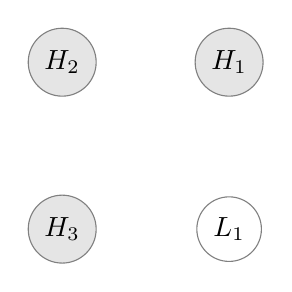
\begin{tikzpicture}[shorten >=1pt,draw=black!50]
	\node (H1) at ( 1.06,  1.06)	[circle, draw, fill = gray!20]	{$H_{1}$};
	\node (H2) at (-1.06,  1.06)	[circle, draw, fill = gray!20]	{$H_{2}$};
	\node (H3) at (-1.06, -1.06)	[circle, draw, fill = gray!20]	{$H_{3}$};
	\node (L1) at ( 1.06, -1.06)	[circle, draw, fill = white]	{$L_{1}$};
\end{tikzpicture}
\end{center}
\columnbreak

\scaleeq{
Equations: \begin{cases}
	e^{H}_{1} \left(\frac{25 \phi}{4} - 4\right) = \alpha - e^{H}_{2} - e^{H}_{3} - e^{L}_{1} \theta - \gamma\\
	e^{H}_{2} \left(\frac{25 \phi}{4} - 4\right) = \alpha - e^{H}_{1} - e^{H}_{3} - e^{L}_{1} \theta - \gamma\\
	e^{H}_{3} \left(\frac{25 \phi}{4} - 4\right) = \alpha - e^{H}_{1} - e^{H}_{2} - e^{L}_{1} \theta - \gamma\\
	e^{L}_{1} \left(\frac{25 \phi}{4 \theta} - 4 \theta\right) = \alpha - e^{H}_{1} - e^{H}_{2} - e^{H}_{3} - \gamma
\end{cases}
}\end{multicols}


Optimal efforts:

\scaleeq{
\begin{cases}
	e^{H}_{1} &= \frac{4 \left(\alpha - \gamma\right) \left(5 \phi - 4 \theta^{2}\right)}{125 \phi^{2} - 80 \phi \theta^{2} - 40 \phi + 16 \theta^{2}}\\
	e^{H}_{2} &= \frac{4 \left(\alpha - \gamma\right) \left(5 \phi - 4 \theta^{2}\right)}{125 \phi^{2} - 80 \phi \theta^{2} - 40 \phi + 16 \theta^{2}}\\
	e^{H}_{3} &= \frac{4 \left(\alpha - \gamma\right) \left(5 \phi - 4 \theta^{2}\right)}{125 \phi^{2} - 80 \phi \theta^{2} - 40 \phi + 16 \theta^{2}}\\
	e^{L}_{1} &= \frac{4 \theta \left(\alpha - \gamma\right) \left(5 \phi - 4\right)}{125 \phi^{2} - 80 \phi \theta^{2} - 40 \phi + 16 \theta^{2}}
\end{cases}
}

Production Costs:

\scaleeq{
\begin{cases}
	c^{H}_{1} &= - \frac{20 \alpha \phi - 16 \alpha \theta^{2} - 125 \gamma \phi^{2} + 80 \gamma \phi \theta^{2} + 20 \gamma \phi}{125 \phi^{2} - 80 \phi \theta^{2} - 40 \phi + 16 \theta^{2}}\\
	c^{H}_{2} &= - \frac{20 \alpha \phi - 16 \alpha \theta^{2} - 125 \gamma \phi^{2} + 80 \gamma \phi \theta^{2} + 20 \gamma \phi}{125 \phi^{2} - 80 \phi \theta^{2} - 40 \phi + 16 \theta^{2}}\\
	c^{H}_{3} &= - \frac{20 \alpha \phi - 16 \alpha \theta^{2} - 125 \gamma \phi^{2} + 80 \gamma \phi \theta^{2} + 20 \gamma \phi}{125 \phi^{2} - 80 \phi \theta^{2} - 40 \phi + 16 \theta^{2}}\\
	c^{L}_{1} &= - \frac{20 \alpha \phi \theta^{2} - 16 \alpha \theta^{2} - 125 \gamma \phi^{2} + 60 \gamma \phi \theta^{2} + 40 \gamma \phi}{125 \phi^{2} - 80 \phi \theta^{2} - 40 \phi + 16 \theta^{2}}
\end{cases}
}

Production Quantities:

\scaleeq{
\begin{cases}
	q^{H}_{1} &= \frac{5 \phi \left(\alpha - \gamma\right) \left(5 \phi - 4 \theta^{2}\right)}{125 \phi^{2} - 80 \phi \theta^{2} - 40 \phi + 16 \theta^{2}}\\
	q^{H}_{2} &= \frac{5 \phi \left(\alpha - \gamma\right) \left(5 \phi - 4 \theta^{2}\right)}{125 \phi^{2} - 80 \phi \theta^{2} - 40 \phi + 16 \theta^{2}}\\
	q^{H}_{3} &= \frac{5 \phi \left(\alpha - \gamma\right) \left(5 \phi - 4 \theta^{2}\right)}{125 \phi^{2} - 80 \phi \theta^{2} - 40 \phi + 16 \theta^{2}}\\
	q^{L}_{1} &= \frac{5 \phi \left(\alpha - \gamma\right) \left(5 \phi - 4\right)}{125 \phi^{2} - 80 \phi \theta^{2} - 40 \phi + 16 \theta^{2}}
\end{cases}
}

Profits:

\begin{equation}
\label{eq:E0A:3H1L_profit}
\scaledequation{\begin{cases}
	\pi^{H}_{1} &= \frac{\phi \left(\alpha - \gamma\right)^{2} \left(5 \phi - 4 \theta^{2}\right)^{2} \left(25 \phi - 16\right)}{\left(125 \phi^{2} - 80 \phi \theta^{2} - 40 \phi + 16 \theta^{2}\right)^{2}}\\
	\pi^{H}_{2} &= \frac{\phi \left(\alpha - \gamma\right)^{2} \left(5 \phi - 4 \theta^{2}\right)^{2} \left(25 \phi - 16\right)}{\left(125 \phi^{2} - 80 \phi \theta^{2} - 40 \phi + 16 \theta^{2}\right)^{2}}\\
	\pi^{H}_{3} &= \frac{\phi \left(\alpha - \gamma\right)^{2} \left(5 \phi - 4 \theta^{2}\right)^{2} \left(25 \phi - 16\right)}{\left(125 \phi^{2} - 80 \phi \theta^{2} - 40 \phi + 16 \theta^{2}\right)^{2}}\\
	\pi^{L}_{1} &= \frac{\phi \left(\alpha - \gamma\right)^{2} \left(5 \phi - 4\right)^{2} \left(25 \phi - 16 \theta^{2}\right)}{\left(125 \phi^{2} - 80 \phi \theta^{2} - 40 \phi + 16 \theta^{2}\right)^{2}}
\end{cases}
}
\end{equation}

Total Production:

\scaleeq{
\frac{20 \phi \left(\alpha - \gamma\right) \left(5 \phi - 3 \theta^{2} - 1\right)}{125 \phi^{2} - 80 \phi \theta^{2} - 40 \phi + 16 \theta^{2}}
}

Price:

\scaleeq{
\frac{25 \alpha \phi^{2} - 20 \alpha \phi \theta^{2} - 20 \alpha \phi + 16 \alpha \theta^{2} + 100 \gamma \phi^{2} - 60 \gamma \phi \theta^{2} - 20 \gamma \phi}{125 \phi^{2} - 80 \phi \theta^{2} - 40 \phi + 16 \theta^{2}}
}

Firm Surplus:

\scaleeq{
\frac{4 \phi \left(\alpha - \gamma\right)^{2} \left(625 \phi^{3} - 850 \phi^{2} \theta^{2} - 550 \phi^{2} + 300 \phi \theta^{4} + 640 \phi \theta^{2} + 100 \phi - 192 \theta^{4} - 64 \theta^{2}\right)}{\left(125 \phi^{2} - 80 \phi \theta^{2} - 40 \phi + 16 \theta^{2}\right)^{2}}
}

Consumer Surplus:

\scaleeq{
\frac{200 \phi^{2} \left(\alpha - \gamma\right)^{2} \left(5 \phi - 3 \theta^{2} - 1\right)^{2}}{\left(125 \phi^{2} - 80 \phi \theta^{2} - 40 \phi + 16 \theta^{2}\right)^{2}}
}

Social Welfare:

\scaleeq{
\frac{4 \phi \left(\alpha - \gamma\right)^{2} \left(1875 \phi^{3} - 2350 \phi^{2} \theta^{2} - 1050 \phi^{2} + 750 \phi \theta^{4} + 940 \phi \theta^{2} + 150 \phi - 192 \theta^{4} - 64 \theta^{2}\right)}{\left(125 \phi^{2} - 80 \phi \theta^{2} - 40 \phi + 16 \theta^{2}\right)^{2}}
}

%======================================================================

\subsubsection{E1A [3H1L]}
\label{apx:E1A:3H1L}

\begin{multicols}{2}
\begin{center}
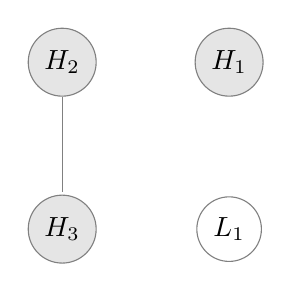
\begin{tikzpicture}[shorten >=1pt,draw=black!50]
	\node (H1) at ( 1.06,  1.06)	[circle, draw, fill = gray!20]	{$H_{1}$};
	\node (H2) at (-1.06,  1.06)	[circle, draw, fill = gray!20]	{$H_{2}$};
	\node (H3) at (-1.06, -1.06)	[circle, draw, fill = gray!20]	{$H_{3}$};
	\node (L1) at ( 1.06, -1.06)	[circle, draw, fill = white]	{$L_{1}$};
	\draw (H2) -- (H3);
\end{tikzpicture}
\end{center}
\columnbreak

\scaleeq{
Equations: \begin{cases}
	e^{H}_{1} \left(\frac{25 \phi}{4} - 4\right) = \alpha - 2 e^{H}_{2} - 2 e^{H}_{3} - e^{L}_{1} \theta - \gamma\\
	e^{H}_{2} \left(\frac{25 \phi}{3} - 3\right) = \alpha - e^{H}_{1} + 3 e^{H}_{3} - e^{L}_{1} \theta - \gamma\\
	e^{H}_{3} \left(\frac{25 \phi}{3} - 3\right) = \alpha - e^{H}_{1} + 3 e^{H}_{2} - e^{L}_{1} \theta - \gamma\\
	e^{L}_{1} \left(\frac{25 \phi}{4 \theta} - 4 \theta\right) = \alpha - e^{H}_{1} - 2 e^{H}_{2} - 2 e^{H}_{3} - \gamma
\end{cases}
}\end{multicols}


Optimal efforts:

\scaleeq{
\begin{cases}
	e^{H}_{1} &= \frac{4 \left(\alpha - \gamma\right) \left(5 \phi - 6\right) \left(5 \phi - 4 \theta^{2}\right)}{625 \phi^{3} - 400 \phi^{2} \theta^{2} - 850 \phi^{2} + 480 \phi \theta^{2} + 240 \phi - 96 \theta^{2}}\\
	e^{H}_{2} &= \frac{3 \left(\alpha - \gamma\right) \left(5 \phi - 4\right) \left(5 \phi - 4 \theta^{2}\right)}{625 \phi^{3} - 400 \phi^{2} \theta^{2} - 850 \phi^{2} + 480 \phi \theta^{2} + 240 \phi - 96 \theta^{2}}\\
	e^{H}_{3} &= \frac{3 \left(\alpha - \gamma\right) \left(5 \phi - 4\right) \left(5 \phi - 4 \theta^{2}\right)}{625 \phi^{3} - 400 \phi^{2} \theta^{2} - 850 \phi^{2} + 480 \phi \theta^{2} + 240 \phi - 96 \theta^{2}}\\
	e^{L}_{1} &= \frac{4 \theta \left(\alpha - \gamma\right) \left(5 \phi - 6\right) \left(5 \phi - 4\right)}{625 \phi^{3} - 400 \phi^{2} \theta^{2} - 850 \phi^{2} + 480 \phi \theta^{2} + 240 \phi - 96 \theta^{2}}
\end{cases}
}

Production Costs:

\scaleeq{
\begin{cases}
	c^{H}_{1} &= - \frac{100 \alpha \phi^{2} - 80 \alpha \phi \theta^{2} - 120 \alpha \phi + 96 \alpha \theta^{2} - 625 \gamma \phi^{3} + 400 \gamma \phi^{2} \theta^{2} + 750 \gamma \phi^{2} - 400 \gamma \phi \theta^{2} - 120 \gamma \phi}{625 \phi^{3} - 400 \phi^{2} \theta^{2} - 850 \phi^{2} + 480 \phi \theta^{2} + 240 \phi - 96 \theta^{2}}\\
	c^{H}_{2} &= - \frac{150 \alpha \phi^{2} - 120 \alpha \phi \theta^{2} - 120 \alpha \phi + 96 \alpha \theta^{2} - 625 \gamma \phi^{3} + 400 \gamma \phi^{2} \theta^{2} + 700 \gamma \phi^{2} - 360 \gamma \phi \theta^{2} - 120 \gamma \phi}{625 \phi^{3} - 400 \phi^{2} \theta^{2} - 850 \phi^{2} + 480 \phi \theta^{2} + 240 \phi - 96 \theta^{2}}\\
	c^{H}_{3} &= - \frac{150 \alpha \phi^{2} - 120 \alpha \phi \theta^{2} - 120 \alpha \phi + 96 \alpha \theta^{2} - 625 \gamma \phi^{3} + 400 \gamma \phi^{2} \theta^{2} + 700 \gamma \phi^{2} - 360 \gamma \phi \theta^{2} - 120 \gamma \phi}{625 \phi^{3} - 400 \phi^{2} \theta^{2} - 850 \phi^{2} + 480 \phi \theta^{2} + 240 \phi - 96 \theta^{2}}\\
	c^{L}_{1} &= - \frac{100 \alpha \phi^{2} \theta^{2} - 200 \alpha \phi \theta^{2} + 96 \alpha \theta^{2} - 625 \gamma \phi^{3} + 300 \gamma \phi^{2} \theta^{2} + 850 \gamma \phi^{2} - 280 \gamma \phi \theta^{2} - 240 \gamma \phi}{625 \phi^{3} - 400 \phi^{2} \theta^{2} - 850 \phi^{2} + 480 \phi \theta^{2} + 240 \phi - 96 \theta^{2}}
\end{cases}
}

Production Quantities:

\scaleeq{
\begin{cases}
	q^{H}_{1} &= \frac{5 \phi \left(\alpha - \gamma\right) \left(5 \phi - 6\right) \left(5 \phi - 4 \theta^{2}\right)}{625 \phi^{3} - 400 \phi^{2} \theta^{2} - 850 \phi^{2} + 480 \phi \theta^{2} + 240 \phi - 96 \theta^{2}}\\
	q^{H}_{2} &= \frac{5 \phi \left(\alpha - \gamma\right) \left(5 \phi - 4\right) \left(5 \phi - 4 \theta^{2}\right)}{625 \phi^{3} - 400 \phi^{2} \theta^{2} - 850 \phi^{2} + 480 \phi \theta^{2} + 240 \phi - 96 \theta^{2}}\\
	q^{H}_{3} &= \frac{5 \phi \left(\alpha - \gamma\right) \left(5 \phi - 4\right) \left(5 \phi - 4 \theta^{2}\right)}{625 \phi^{3} - 400 \phi^{2} \theta^{2} - 850 \phi^{2} + 480 \phi \theta^{2} + 240 \phi - 96 \theta^{2}}\\
	q^{L}_{1} &= \frac{5 \phi \left(\alpha - \gamma\right) \left(5 \phi - 6\right) \left(5 \phi - 4\right)}{625 \phi^{3} - 400 \phi^{2} \theta^{2} - 850 \phi^{2} + 480 \phi \theta^{2} + 240 \phi - 96 \theta^{2}}
\end{cases}
}

Profits:

\begin{equation}
\label{eq:E1A:3H1L_profit}
\scaledequation{\begin{cases}
	\pi^{H}_{1} &= \frac{\phi \left(\alpha - \gamma\right)^{2} \left(5 \phi - 6\right)^{2} \left(5 \phi - 4 \theta^{2}\right)^{2} \left(25 \phi - 16\right)}{\left(625 \phi^{3} - 400 \phi^{2} \theta^{2} - 850 \phi^{2} + 480 \phi \theta^{2} + 240 \phi - 96 \theta^{2}\right)^{2}}\\
	\pi^{H}_{2} &= \frac{\phi \left(\alpha - \gamma\right)^{2} \left(5 \phi - 4\right)^{2} \left(5 \phi - 4 \theta^{2}\right)^{2} \left(25 \phi - 9\right)}{\left(625 \phi^{3} - 400 \phi^{2} \theta^{2} - 850 \phi^{2} + 480 \phi \theta^{2} + 240 \phi - 96 \theta^{2}\right)^{2}}\\
	\pi^{H}_{3} &= \frac{\phi \left(\alpha - \gamma\right)^{2} \left(5 \phi - 4\right)^{2} \left(5 \phi - 4 \theta^{2}\right)^{2} \left(25 \phi - 9\right)}{\left(625 \phi^{3} - 400 \phi^{2} \theta^{2} - 850 \phi^{2} + 480 \phi \theta^{2} + 240 \phi - 96 \theta^{2}\right)^{2}}\\
	\pi^{L}_{1} &= \frac{\phi \left(\alpha - \gamma\right)^{2} \left(5 \phi - 6\right)^{2} \left(5 \phi - 4\right)^{2} \left(25 \phi - 16 \theta^{2}\right)}{\left(625 \phi^{3} - 400 \phi^{2} \theta^{2} - 850 \phi^{2} + 480 \phi \theta^{2} + 240 \phi - 96 \theta^{2}\right)^{2}}
\end{cases}
}
\end{equation}

Total Production:

\scaleeq{
\frac{20 \phi \left(\alpha - \gamma\right) \left(25 \phi^{2} - 15 \phi \theta^{2} - 30 \phi + 14 \theta^{2} + 6\right)}{625 \phi^{3} - 400 \phi^{2} \theta^{2} - 850 \phi^{2} + 480 \phi \theta^{2} + 240 \phi - 96 \theta^{2}}
}

Price:

\scaleeq{
\frac{125 \alpha \phi^{3} - 100 \alpha \phi^{2} \theta^{2} - 250 \alpha \phi^{2} + 200 \alpha \phi \theta^{2} + 120 \alpha \phi - 96 \alpha \theta^{2} + 500 \gamma \phi^{3} - 300 \gamma \phi^{2} \theta^{2} - 600 \gamma \phi^{2} + 280 \gamma \phi \theta^{2} + 120 \gamma \phi}{625 \phi^{3} - 400 \phi^{2} \theta^{2} - 850 \phi^{2} + 480 \phi \theta^{2} + 240 \phi - 96 \theta^{2}}
}

Firm Surplus:

\scaleeq{
\frac{2 \phi \left(\alpha - \gamma\right)^{2} \left(31250 \phi^{5} - 42500 \phi^{4} \theta^{2} - 85625 \phi^{4} + 15000 \phi^{3} \theta^{4} + 107000 \phi^{3} \theta^{2} + 88500 \phi^{3} - 34800 \phi^{2} \theta^{4} - 97200 \phi^{2} \theta^{2} - 40800 \phi^{2} + 27040 \phi \theta^{4} + 36480 \phi \theta^{2} + 7200 \phi - 6912 \theta^{4} - 4608 \theta^{2}\right)}{\left(625 \phi^{3} - 400 \phi^{2} \theta^{2} - 850 \phi^{2} + 480 \phi \theta^{2} + 240 \phi - 96 \theta^{2}\right)^{2}}
}

Consumer Surplus:

\scaleeq{
\frac{200 \phi^{2} \left(\alpha - \gamma\right)^{2} \left(25 \phi^{2} - 15 \phi \theta^{2} - 30 \phi + 14 \theta^{2} + 6\right)^{2}}{\left(625 \phi^{3} - 400 \phi^{2} \theta^{2} - 850 \phi^{2} + 480 \phi \theta^{2} + 240 \phi - 96 \theta^{2}\right)^{2}}
}

Social Welfare:

\scaleeq{
\frac{2 \phi \left(\alpha - \gamma\right)^{2} \left(93750 \phi^{5} - 117500 \phi^{4} \theta^{2} - 235625 \phi^{4} + 37500 \phi^{3} \theta^{4} + 267000 \phi^{3} \theta^{2} + 208500 \phi^{3} - 76800 \phi^{2} \theta^{4} - 199200 \phi^{2} \theta^{2} - 76800 \phi^{2} + 46640 \phi \theta^{4} + 53280 \phi \theta^{2} + 10800 \phi - 6912 \theta^{4} - 4608 \theta^{2}\right)}{\left(625 \phi^{3} - 400 \phi^{2} \theta^{2} - 850 \phi^{2} + 480 \phi \theta^{2} + 240 \phi - 96 \theta^{2}\right)^{2}}
}

%======================================================================

\subsubsection{E1B [3H1L]}
\label{apx:E1B:3H1L}

\begin{multicols}{2}
\begin{center}
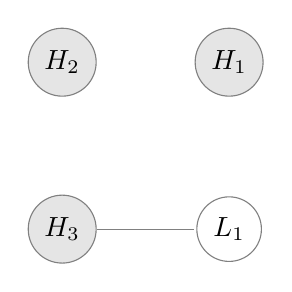
\begin{tikzpicture}[shorten >=1pt,draw=black!50]
	\node (H1) at ( 1.06,  1.06)	[circle, draw, fill = gray!20]	{$H_{1}$};
	\node (H2) at (-1.06,  1.06)	[circle, draw, fill = gray!20]	{$H_{2}$};
	\node (H3) at (-1.06, -1.06)	[circle, draw, fill = gray!20]	{$H_{3}$};
	\node (L1) at ( 1.06, -1.06)	[circle, draw, fill = white]	{$L_{1}$};
	\draw (H3) -- (L1);
\end{tikzpicture}
\end{center}
\columnbreak

\scaleeq{
Equations: \begin{cases}
	e^{H}_{1} \left(\frac{25 \phi}{4} - 4\right) = \alpha - e^{H}_{2} - 2 e^{H}_{3} - 2 e^{L}_{1} \theta - \gamma\\
	e^{H}_{2} \left(\frac{25 \phi}{4} - 4\right) = \alpha - e^{H}_{1} - 2 e^{H}_{3} - 2 e^{L}_{1} \theta - \gamma\\
	e^{H}_{3} \left(\frac{25 \phi}{3} - 3\right) = \alpha - e^{H}_{1} - e^{H}_{2} + 3 e^{L}_{1} \theta - \gamma\\
	e^{L}_{1} \left(\frac{25 \phi}{3 \theta} - 3 \theta\right) = \alpha - e^{H}_{1} - e^{H}_{2} + 3 e^{H}_{3} - \gamma
\end{cases}
}\end{multicols}


Optimal efforts:

\scaleeq{
\begin{cases}
	e^{H}_{1} &= \frac{4 \left(\alpha - \gamma\right) \left(5 \phi - 3 \theta^{2} - 3\right)}{125 \phi^{2} - 45 \phi \theta^{2} - 105 \phi + 12 \theta^{2} + 12}\\
	e^{H}_{2} &= \frac{4 \left(\alpha - \gamma\right) \left(5 \phi - 3 \theta^{2} - 3\right)}{125 \phi^{2} - 45 \phi \theta^{2} - 105 \phi + 12 \theta^{2} + 12}\\
	e^{H}_{3} &= \frac{3 \left(\alpha - \gamma\right) \left(5 \phi - 4\right)}{125 \phi^{2} - 45 \phi \theta^{2} - 105 \phi + 12 \theta^{2} + 12}\\
	e^{L}_{1} &= \frac{3 \theta \left(\alpha - \gamma\right) \left(5 \phi - 4\right)}{125 \phi^{2} - 45 \phi \theta^{2} - 105 \phi + 12 \theta^{2} + 12}
\end{cases}
}

Production Costs:

\scaleeq{
\begin{cases}
	c^{H}_{1} &= - \frac{20 \alpha \phi - 12 \alpha \theta^{2} - 12 \alpha - 125 \gamma \phi^{2} + 45 \gamma \phi \theta^{2} + 85 \gamma \phi}{125 \phi^{2} - 45 \phi \theta^{2} - 105 \phi + 12 \theta^{2} + 12}\\
	c^{H}_{2} &= - \frac{20 \alpha \phi - 12 \alpha \theta^{2} - 12 \alpha - 125 \gamma \phi^{2} + 45 \gamma \phi \theta^{2} + 85 \gamma \phi}{125 \phi^{2} - 45 \phi \theta^{2} - 105 \phi + 12 \theta^{2} + 12}\\
	c^{H}_{3} &= - \frac{15 \alpha \phi \theta^{2} + 15 \alpha \phi - 12 \alpha \theta^{2} - 12 \alpha - 125 \gamma \phi^{2} + 30 \gamma \phi \theta^{2} + 90 \gamma \phi}{125 \phi^{2} - 45 \phi \theta^{2} - 105 \phi + 12 \theta^{2} + 12}\\
	c^{L}_{1} &= - \frac{15 \alpha \phi \theta^{2} + 15 \alpha \phi - 12 \alpha \theta^{2} - 12 \alpha - 125 \gamma \phi^{2} + 30 \gamma \phi \theta^{2} + 90 \gamma \phi}{125 \phi^{2} - 45 \phi \theta^{2} - 105 \phi + 12 \theta^{2} + 12}
\end{cases}
}

Production Quantities:

\scaleeq{
\begin{cases}
	q^{H}_{1} &= \frac{5 \phi \left(\alpha - \gamma\right) \left(5 \phi - 3 \theta^{2} - 3\right)}{125 \phi^{2} - 45 \phi \theta^{2} - 105 \phi + 12 \theta^{2} + 12}\\
	q^{H}_{2} &= \frac{5 \phi \left(\alpha - \gamma\right) \left(5 \phi - 3 \theta^{2} - 3\right)}{125 \phi^{2} - 45 \phi \theta^{2} - 105 \phi + 12 \theta^{2} + 12}\\
	q^{H}_{3} &= \frac{5 \phi \left(\alpha - \gamma\right) \left(5 \phi - 4\right)}{125 \phi^{2} - 45 \phi \theta^{2} - 105 \phi + 12 \theta^{2} + 12}\\
	q^{L}_{1} &= \frac{5 \phi \left(\alpha - \gamma\right) \left(5 \phi - 4\right)}{125 \phi^{2} - 45 \phi \theta^{2} - 105 \phi + 12 \theta^{2} + 12}
\end{cases}
}

Profits:

\begin{equation}
\label{eq:E1B:3H1L_profit}
\scaledequation{\begin{cases}
	\pi^{H}_{1} &= \frac{\phi \left(\alpha - \gamma\right)^{2} \left(25 \phi - 16\right) \left(5 \phi - 3 \theta^{2} - 3\right)^{2}}{\left(125 \phi^{2} - 45 \phi \theta^{2} - 105 \phi + 12 \theta^{2} + 12\right)^{2}}\\
	\pi^{H}_{2} &= \frac{\phi \left(\alpha - \gamma\right)^{2} \left(25 \phi - 16\right) \left(5 \phi - 3 \theta^{2} - 3\right)^{2}}{\left(125 \phi^{2} - 45 \phi \theta^{2} - 105 \phi + 12 \theta^{2} + 12\right)^{2}}\\
	\pi^{H}_{3} &= \frac{\phi \left(\alpha - \gamma\right)^{2} \left(5 \phi - 4\right)^{2} \left(25 \phi - 9\right)}{\left(125 \phi^{2} - 45 \phi \theta^{2} - 105 \phi + 12 \theta^{2} + 12\right)^{2}}\\
	\pi^{L}_{1} &= \frac{\phi \left(\alpha - \gamma\right)^{2} \left(5 \phi - 4\right)^{2} \left(25 \phi - 9 \theta^{2}\right)}{\left(125 \phi^{2} - 45 \phi \theta^{2} - 105 \phi + 12 \theta^{2} + 12\right)^{2}}
\end{cases}
}
\end{equation}

Total Production:

\scaleeq{
\frac{10 \phi \left(\alpha - \gamma\right) \left(10 \phi - 3 \theta^{2} - 7\right)}{125 \phi^{2} - 45 \phi \theta^{2} - 105 \phi + 12 \theta^{2} + 12}
}

Price:

\scaleeq{
\frac{25 \alpha \phi^{2} - 15 \alpha \phi \theta^{2} - 35 \alpha \phi + 12 \alpha \theta^{2} + 12 \alpha + 100 \gamma \phi^{2} - 30 \gamma \phi \theta^{2} - 70 \gamma \phi}{125 \phi^{2} - 45 \phi \theta^{2} - 105 \phi + 12 \theta^{2} + 12}
}

Firm Surplus:

\scaleeq{
\frac{\phi \left(\alpha - \gamma\right)^{2} \left(2500 \phi^{3} - 1725 \phi^{2} \theta^{2} - 4525 \phi^{2} + 450 \phi \theta^{4} + 2220 \phi \theta^{2} + 2570 \phi - 288 \theta^{4} - 720 \theta^{2} - 432\right)}{\left(125 \phi^{2} - 45 \phi \theta^{2} - 105 \phi + 12 \theta^{2} + 12\right)^{2}}
}

Consumer Surplus:

\scaleeq{
\frac{50 \phi^{2} \left(\alpha - \gamma\right)^{2} \left(10 \phi - 3 \theta^{2} - 7\right)^{2}}{\left(125 \phi^{2} - 45 \phi \theta^{2} - 105 \phi + 12 \theta^{2} + 12\right)^{2}}
}

Social Welfare:

\scaleeq{
\frac{\phi \left(\alpha - \gamma\right)^{2} \left(7500 \phi^{3} - 4725 \phi^{2} \theta^{2} - 11525 \phi^{2} + 900 \phi \theta^{4} + 4320 \phi \theta^{2} + 5020 \phi - 288 \theta^{4} - 720 \theta^{2} - 432\right)}{\left(125 \phi^{2} - 45 \phi \theta^{2} - 105 \phi + 12 \theta^{2} + 12\right)^{2}}
}

%======================================================================

\subsubsection{E2A [3H1L]}
\label{apx:E2A:3H1L}

\begin{multicols}{2}
\begin{center}
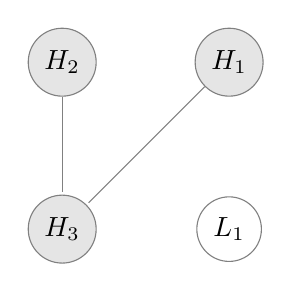
\begin{tikzpicture}[shorten >=1pt,draw=black!50]
	\node (H1) at ( 1.06,  1.06)	[circle, draw, fill = gray!20]	{$H_{1}$};
	\node (H2) at (-1.06,  1.06)	[circle, draw, fill = gray!20]	{$H_{2}$};
	\node (H3) at (-1.06, -1.06)	[circle, draw, fill = gray!20]	{$H_{3}$};
	\node (L1) at ( 1.06, -1.06)	[circle, draw, fill = white]	{$L_{1}$};
	\draw (H1) -- (H3);
	\draw (H2) -- (H3);
\end{tikzpicture}
\end{center}
\columnbreak

\scaleeq{
Equations: \begin{cases}
	e^{H}_{1} \left(\frac{25 \phi}{3} - 3\right) = \alpha - 2 e^{H}_{2} + 2 e^{H}_{3} - e^{L}_{1} \theta - \gamma\\
	e^{H}_{2} \left(\frac{25 \phi}{3} - 3\right) = \alpha - 2 e^{H}_{1} + 2 e^{H}_{3} - e^{L}_{1} \theta - \gamma\\
	e^{H}_{3} \left(\frac{25 \phi}{2} - 2\right) = \alpha + 3 e^{H}_{1} + 3 e^{H}_{2} - e^{L}_{1} \theta - \gamma\\
	e^{L}_{1} \left(\frac{25 \phi}{4 \theta} - 4 \theta\right) = \alpha - 2 e^{H}_{1} - 2 e^{H}_{2} - 3 e^{H}_{3} - \gamma
\end{cases}
}\end{multicols}


Optimal efforts:

\scaleeq{
\begin{cases}
	e^{H}_{1} &= \frac{15 \phi \left(\alpha - \gamma\right) \left(5 \phi - 4 \theta^{2}\right)}{\left(5 \phi + 1\right) \left(125 \phi^{2} - 80 \phi \theta^{2} - 60 \phi + 24 \theta^{2}\right)}\\
	e^{H}_{2} &= \frac{15 \phi \left(\alpha - \gamma\right) \left(5 \phi - 4 \theta^{2}\right)}{\left(5 \phi + 1\right) \left(125 \phi^{2} - 80 \phi \theta^{2} - 60 \phi + 24 \theta^{2}\right)}\\
	e^{H}_{3} &= \frac{2 \left(\alpha - \gamma\right) \left(5 \phi + 3\right) \left(5 \phi - 4 \theta^{2}\right)}{\left(5 \phi + 1\right) \left(125 \phi^{2} - 80 \phi \theta^{2} - 60 \phi + 24 \theta^{2}\right)}\\
	e^{L}_{1} &= \frac{4 \theta \left(\alpha - \gamma\right) \left(5 \phi - 6\right)}{125 \phi^{2} - 80 \phi \theta^{2} - 60 \phi + 24 \theta^{2}}
\end{cases}
}

Production Costs:

\scaleeq{
\begin{cases}
	c^{H}_{1} &= - \frac{125 \alpha \phi^{2} - 100 \alpha \phi \theta^{2} + 30 \alpha \phi - 24 \alpha \theta^{2} - 625 \gamma \phi^{3} + 400 \gamma \phi^{2} \theta^{2} + 50 \gamma \phi^{2} + 60 \gamma \phi \theta^{2} + 30 \gamma \phi}{\left(5 \phi + 1\right) \left(125 \phi^{2} - 80 \phi \theta^{2} - 60 \phi + 24 \theta^{2}\right)}\\
	c^{H}_{2} &= - \frac{125 \alpha \phi^{2} - 100 \alpha \phi \theta^{2} + 30 \alpha \phi - 24 \alpha \theta^{2} - 625 \gamma \phi^{3} + 400 \gamma \phi^{2} \theta^{2} + 50 \gamma \phi^{2} + 60 \gamma \phi \theta^{2} + 30 \gamma \phi}{\left(5 \phi + 1\right) \left(125 \phi^{2} - 80 \phi \theta^{2} - 60 \phi + 24 \theta^{2}\right)}\\
	c^{H}_{3} &= - \frac{200 \alpha \phi^{2} - 160 \alpha \phi \theta^{2} + 30 \alpha \phi - 24 \alpha \theta^{2} - 625 \gamma \phi^{3} + 400 \gamma \phi^{2} \theta^{2} - 25 \gamma \phi^{2} + 120 \gamma \phi \theta^{2} + 30 \gamma \phi}{\left(5 \phi + 1\right) \left(125 \phi^{2} - 80 \phi \theta^{2} - 60 \phi + 24 \theta^{2}\right)}\\
	c^{L}_{1} &= - \frac{20 \alpha \phi \theta^{2} - 24 \alpha \theta^{2} - 125 \gamma \phi^{2} + 60 \gamma \phi \theta^{2} + 60 \gamma \phi}{125 \phi^{2} - 80 \phi \theta^{2} - 60 \phi + 24 \theta^{2}}
\end{cases}
}

Production Quantities:

\scaleeq{
\begin{cases}
	q^{H}_{1} &= \frac{25 \phi^{2} \left(\alpha - \gamma\right) \left(5 \phi - 4 \theta^{2}\right)}{\left(5 \phi + 1\right) \left(125 \phi^{2} - 80 \phi \theta^{2} - 60 \phi + 24 \theta^{2}\right)}\\
	q^{H}_{2} &= \frac{25 \phi^{2} \left(\alpha - \gamma\right) \left(5 \phi - 4 \theta^{2}\right)}{\left(5 \phi + 1\right) \left(125 \phi^{2} - 80 \phi \theta^{2} - 60 \phi + 24 \theta^{2}\right)}\\
	q^{H}_{3} &= \frac{5 \phi \left(\alpha - \gamma\right) \left(5 \phi + 3\right) \left(5 \phi - 4 \theta^{2}\right)}{\left(5 \phi + 1\right) \left(125 \phi^{2} - 80 \phi \theta^{2} - 60 \phi + 24 \theta^{2}\right)}\\
	q^{L}_{1} &= \frac{5 \phi \left(\alpha - \gamma\right) \left(5 \phi - 6\right)}{125 \phi^{2} - 80 \phi \theta^{2} - 60 \phi + 24 \theta^{2}}
\end{cases}
}

Profits:

\begin{equation}
\label{eq:E2A:3H1L_profit}
\scaledequation{\begin{cases}
	\pi^{H}_{1} &= \frac{25 \phi^{3} \left(\alpha - \gamma\right)^{2} \left(5 \phi - 4 \theta^{2}\right)^{2} \left(25 \phi - 9\right)}{\left(5 \phi + 1\right)^{2} \left(125 \phi^{2} - 80 \phi \theta^{2} - 60 \phi + 24 \theta^{2}\right)^{2}}\\
	\pi^{H}_{2} &= \frac{25 \phi^{3} \left(\alpha - \gamma\right)^{2} \left(5 \phi - 4 \theta^{2}\right)^{2} \left(25 \phi - 9\right)}{\left(5 \phi + 1\right)^{2} \left(125 \phi^{2} - 80 \phi \theta^{2} - 60 \phi + 24 \theta^{2}\right)^{2}}\\
	\pi^{H}_{3} &= \frac{\phi \left(\alpha - \gamma\right)^{2} \left(5 \phi + 3\right)^{2} \left(5 \phi - 4 \theta^{2}\right)^{2} \left(25 \phi - 4\right)}{\left(5 \phi + 1\right)^{2} \left(125 \phi^{2} - 80 \phi \theta^{2} - 60 \phi + 24 \theta^{2}\right)^{2}}\\
	\pi^{L}_{1} &= \frac{\phi \left(\alpha - \gamma\right)^{2} \left(5 \phi - 6\right)^{2} \left(25 \phi - 16 \theta^{2}\right)}{\left(125 \phi^{2} - 80 \phi \theta^{2} - 60 \phi + 24 \theta^{2}\right)^{2}}
\end{cases}
}
\end{equation}

Total Production:

\scaleeq{
\frac{10 \phi \left(\alpha - \gamma\right) \left(10 \phi - 6 \theta^{2} - 3\right)}{125 \phi^{2} - 80 \phi \theta^{2} - 60 \phi + 24 \theta^{2}}
}

Price:

\scaleeq{
\frac{25 \alpha \phi^{2} - 20 \alpha \phi \theta^{2} - 30 \alpha \phi + 24 \alpha \theta^{2} + 100 \gamma \phi^{2} - 60 \gamma \phi \theta^{2} - 30 \gamma \phi}{125 \phi^{2} - 80 \phi \theta^{2} - 60 \phi + 24 \theta^{2}}
}

Firm Surplus:

\scaleeq{
\frac{2 \phi \left(\alpha - \gamma\right)^{2} \left(31250 \phi^{5} - 42500 \phi^{4} \theta^{2} - 13125 \phi^{4} + 15000 \phi^{3} \theta^{4} + 6000 \phi^{3} \theta^{2} + 5375 \phi^{3} + 1600 \phi^{2} \theta^{4} - 4700 \phi^{2} \theta^{2} + 3300 \phi^{2} + 840 \phi \theta^{4} - 1680 \phi \theta^{2} + 450 \phi - 288 \theta^{4} - 288 \theta^{2}\right)}{\left(5 \phi + 1\right)^{2} \left(125 \phi^{2} - 80 \phi \theta^{2} - 60 \phi + 24 \theta^{2}\right)^{2}}
}

Consumer Surplus:

\scaleeq{
\frac{50 \phi^{2} \left(\alpha - \gamma\right)^{2} \left(10 \phi - 6 \theta^{2} - 3\right)^{2}}{\left(125 \phi^{2} - 80 \phi \theta^{2} - 60 \phi + 24 \theta^{2}\right)^{2}}
}

Social Welfare:

\scaleeq{
\frac{2 \phi \left(\alpha - \gamma\right)^{2} \left(93750 \phi^{5} - 117500 \phi^{4} \theta^{2} - 25625 \phi^{4} + 37500 \phi^{3} \theta^{4} - 1500 \phi^{3} \theta^{2} - 1500 \phi^{3} + 10600 \phi^{2} \theta^{4} + 1300 \phi^{2} \theta^{2} + 4050 \phi^{2} + 1740 \phi \theta^{4} - 780 \phi \theta^{2} + 675 \phi - 288 \theta^{4} - 288 \theta^{2}\right)}{\left(5 \phi + 1\right)^{2} \left(125 \phi^{2} - 80 \phi \theta^{2} - 60 \phi + 24 \theta^{2}\right)^{2}}
}

%======================================================================

\subsubsection{E2B [3H1L]}
\label{apx:E2B:3H1L}

\begin{multicols}{2}
\begin{center}
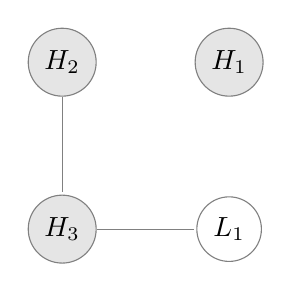
\begin{tikzpicture}[shorten >=1pt,draw=black!50]
	\node (H1) at ( 1.06,  1.06)	[circle, draw, fill = gray!20]	{$H_{1}$};
	\node (H2) at (-1.06,  1.06)	[circle, draw, fill = gray!20]	{$H_{2}$};
	\node (H3) at (-1.06, -1.06)	[circle, draw, fill = gray!20]	{$H_{3}$};
	\node (L1) at ( 1.06, -1.06)	[circle, draw, fill = white]	{$L_{1}$};
	\draw (H2) -- (H3);
	\draw (H3) -- (L1);
\end{tikzpicture}
\end{center}
\columnbreak

\scaleeq{
Equations: \begin{cases}
	e^{H}_{1} \left(\frac{25 \phi}{4} - 4\right) = \alpha - 2 e^{H}_{2} - 3 e^{H}_{3} - 2 e^{L}_{1} \theta - \gamma\\
	e^{H}_{2} \left(\frac{25 \phi}{3} - 3\right) = \alpha - e^{H}_{1} + 2 e^{H}_{3} - 2 e^{L}_{1} \theta - \gamma\\
	e^{H}_{3} \left(\frac{25 \phi}{2} - 2\right) = \alpha - e^{H}_{1} + 3 e^{H}_{2} + 3 e^{L}_{1} \theta - \gamma\\
	e^{L}_{1} \left(\frac{25 \phi}{3 \theta} - 3 \theta\right) = \alpha - e^{H}_{1} - 2 e^{H}_{2} + 2 e^{H}_{3} - \gamma
\end{cases}
}\end{multicols}


Optimal efforts:

\scaleeq{
\begin{cases}
	e^{H}_{1} &= \frac{4 \left(\alpha - \gamma\right) \left(125 \phi^{3} - 75 \phi^{2} \theta^{2} - 125 \phi^{2} + 45 \phi \theta^{2} + 18 \theta^{2}\right)}{3125 \phi^{4} - 1125 \phi^{3} \theta^{2} - 3625 \phi^{3} + 825 \phi^{2} \theta^{2} + 800 \phi^{2} + 180 \phi \theta^{2} - 72 \theta^{2}}\\
	e^{H}_{2} &= \frac{15 \phi \left(\alpha - \gamma\right) \left(5 \phi - 4\right) \left(5 \phi - 3 \theta^{2}\right)}{3125 \phi^{4} - 1125 \phi^{3} \theta^{2} - 3625 \phi^{3} + 825 \phi^{2} \theta^{2} + 800 \phi^{2} + 180 \phi \theta^{2} - 72 \theta^{2}}\\
	e^{H}_{3} &= \frac{2 \left(\alpha - \gamma\right) \left(5 \phi - 4\right) \left(5 \phi - 3 \theta\right) \left(5 \phi + 3 \theta\right)}{3125 \phi^{4} - 1125 \phi^{3} \theta^{2} - 3625 \phi^{3} + 825 \phi^{2} \theta^{2} + 800 \phi^{2} + 180 \phi \theta^{2} - 72 \theta^{2}}\\
	e^{L}_{1} &= \frac{15 \phi \theta \left(\alpha - \gamma\right) \left(5 \phi - 4\right) \left(5 \phi - 3\right)}{3125 \phi^{4} - 1125 \phi^{3} \theta^{2} - 3625 \phi^{3} + 825 \phi^{2} \theta^{2} + 800 \phi^{2} + 180 \phi \theta^{2} - 72 \theta^{2}}
\end{cases}
}

Production Costs:

\scaleeq{
\begin{cases}
	c^{H}_{1} &= - \frac{500 \alpha \phi^{3} - 300 \alpha \phi^{2} \theta^{2} - 500 \alpha \phi^{2} + 180 \alpha \phi \theta^{2} + 72 \alpha \theta^{2} - 3125 \gamma \phi^{4} + 1125 \gamma \phi^{3} \theta^{2} + 3125 \gamma \phi^{3} - 525 \gamma \phi^{2} \theta^{2} - 300 \gamma \phi^{2} - 360 \gamma \phi \theta^{2}}{3125 \phi^{4} - 1125 \phi^{3} \theta^{2} - 3625 \phi^{3} + 825 \phi^{2} \theta^{2} + 800 \phi^{2} + 180 \phi \theta^{2} - 72 \theta^{2}}\\
	c^{H}_{2} &= - \frac{625 \alpha \phi^{3} - 225 \alpha \phi^{2} \theta^{2} - 500 \alpha \phi^{2} + 90 \alpha \phi \theta^{2} + 72 \alpha \theta^{2} - 3125 \gamma \phi^{4} + 1125 \gamma \phi^{3} \theta^{2} + 3000 \gamma \phi^{3} - 600 \gamma \phi^{2} \theta^{2} - 300 \gamma \phi^{2} - 270 \gamma \phi \theta^{2}}{3125 \phi^{4} - 1125 \phi^{3} \theta^{2} - 3625 \phi^{3} + 825 \phi^{2} \theta^{2} + 800 \phi^{2} + 180 \phi \theta^{2} - 72 \theta^{2}}\\
	c^{H}_{3} &= - \frac{375 \alpha \phi^{3} \theta^{2} + 625 \alpha \phi^{3} - 750 \alpha \phi^{2} \theta^{2} - 500 \alpha \phi^{2} + 270 \alpha \phi \theta^{2} + 72 \alpha \theta^{2} - 3125 \gamma \phi^{4} + 750 \gamma \phi^{3} \theta^{2} + 3000 \gamma \phi^{3} - 75 \gamma \phi^{2} \theta^{2} - 300 \gamma \phi^{2} - 450 \gamma \phi \theta^{2}}{3125 \phi^{4} - 1125 \phi^{3} \theta^{2} - 3625 \phi^{3} + 825 \phi^{2} \theta^{2} + 800 \phi^{2} + 180 \phi \theta^{2} - 72 \theta^{2}}\\
	c^{L}_{1} &= - \frac{375 \alpha \phi^{3} \theta^{2} + 250 \alpha \phi^{3} - 525 \alpha \phi^{2} \theta^{2} - 200 \alpha \phi^{2} + 90 \alpha \phi \theta^{2} + 72 \alpha \theta^{2} - 3125 \gamma \phi^{4} + 750 \gamma \phi^{3} \theta^{2} + 3375 \gamma \phi^{3} - 300 \gamma \phi^{2} \theta^{2} - 600 \gamma \phi^{2} - 270 \gamma \phi \theta^{2}}{3125 \phi^{4} - 1125 \phi^{3} \theta^{2} - 3625 \phi^{3} + 825 \phi^{2} \theta^{2} + 800 \phi^{2} + 180 \phi \theta^{2} - 72 \theta^{2}}
\end{cases}
}

Production Quantities:

\scaleeq{
\begin{cases}
	q^{H}_{1} &= \frac{5 \phi \left(\alpha - \gamma\right) \left(125 \phi^{3} - 75 \phi^{2} \theta^{2} - 125 \phi^{2} + 45 \phi \theta^{2} + 18 \theta^{2}\right)}{3125 \phi^{4} - 1125 \phi^{3} \theta^{2} - 3625 \phi^{3} + 825 \phi^{2} \theta^{2} + 800 \phi^{2} + 180 \phi \theta^{2} - 72 \theta^{2}}\\
	q^{H}_{2} &= \frac{25 \phi^{2} \left(\alpha - \gamma\right) \left(5 \phi - 4\right) \left(5 \phi - 3 \theta^{2}\right)}{3125 \phi^{4} - 1125 \phi^{3} \theta^{2} - 3625 \phi^{3} + 825 \phi^{2} \theta^{2} + 800 \phi^{2} + 180 \phi \theta^{2} - 72 \theta^{2}}\\
	q^{H}_{3} &= \frac{5 \phi \left(\alpha - \gamma\right) \left(5 \phi - 4\right) \left(5 \phi - 3 \theta\right) \left(5 \phi + 3 \theta\right)}{3125 \phi^{4} - 1125 \phi^{3} \theta^{2} - 3625 \phi^{3} + 825 \phi^{2} \theta^{2} + 800 \phi^{2} + 180 \phi \theta^{2} - 72 \theta^{2}}\\
	q^{L}_{1} &= \frac{25 \phi^{2} \left(\alpha - \gamma\right) \left(5 \phi - 4\right) \left(5 \phi - 3\right)}{3125 \phi^{4} - 1125 \phi^{3} \theta^{2} - 3625 \phi^{3} + 825 \phi^{2} \theta^{2} + 800 \phi^{2} + 180 \phi \theta^{2} - 72 \theta^{2}}
\end{cases}
}

Profits:

\begin{equation}
\label{eq:E2B:3H1L_profit}
\scaledequation{\begin{cases}
	\pi^{H}_{1} &= \frac{\phi \left(\alpha - \gamma\right)^{2} \left(25 \phi - 16\right) \left(125 \phi^{3} - 75 \phi^{2} \theta^{2} - 125 \phi^{2} + 45 \phi \theta^{2} + 18 \theta^{2}\right)^{2}}{\left(3125 \phi^{4} - 1125 \phi^{3} \theta^{2} - 3625 \phi^{3} + 825 \phi^{2} \theta^{2} + 800 \phi^{2} + 180 \phi \theta^{2} - 72 \theta^{2}\right)^{2}}\\
	\pi^{H}_{2} &= \frac{25 \phi^{3} \left(\alpha - \gamma\right)^{2} \left(5 \phi - 4\right)^{2} \left(5 \phi - 3 \theta^{2}\right)^{2} \left(25 \phi - 9\right)}{\left(3125 \phi^{4} - 1125 \phi^{3} \theta^{2} - 3625 \phi^{3} + 825 \phi^{2} \theta^{2} + 800 \phi^{2} + 180 \phi \theta^{2} - 72 \theta^{2}\right)^{2}}\\
	\pi^{H}_{3} &= \frac{\phi \left(\alpha - \gamma\right)^{2} \left(5 \phi - 4\right)^{2} \left(5 \phi - 3 \theta\right)^{2} \left(5 \phi + 3 \theta\right)^{2} \left(25 \phi - 4\right)}{\left(3125 \phi^{4} - 1125 \phi^{3} \theta^{2} - 3625 \phi^{3} + 825 \phi^{2} \theta^{2} + 800 \phi^{2} + 180 \phi \theta^{2} - 72 \theta^{2}\right)^{2}}\\
	\pi^{L}_{1} &= \frac{25 \phi^{3} \left(\alpha - \gamma\right)^{2} \left(5 \phi - 4\right)^{2} \left(5 \phi - 3\right)^{2} \left(25 \phi - 9 \theta^{2}\right)}{\left(3125 \phi^{4} - 1125 \phi^{3} \theta^{2} - 3625 \phi^{3} + 825 \phi^{2} \theta^{2} + 800 \phi^{2} + 180 \phi \theta^{2} - 72 \theta^{2}\right)^{2}}
\end{cases}
}
\end{equation}

Total Production:

\scaleeq{
\frac{10 \phi \left(\alpha - \gamma\right) \left(250 \phi^{3} - 75 \phi^{2} \theta^{2} - 250 \phi^{2} + 30 \phi \theta^{2} + 30 \phi + 27 \theta^{2}\right)}{3125 \phi^{4} - 1125 \phi^{3} \theta^{2} - 3625 \phi^{3} + 825 \phi^{2} \theta^{2} + 800 \phi^{2} + 180 \phi \theta^{2} - 72 \theta^{2}}
}

Price:

\scaleeq{
\frac{625 \alpha \phi^{4} - 375 \alpha \phi^{3} \theta^{2} - 1125 \alpha \phi^{3} + 525 \alpha \phi^{2} \theta^{2} + 500 \alpha \phi^{2} - 90 \alpha \phi \theta^{2} - 72 \alpha \theta^{2} + 2500 \gamma \phi^{4} - 750 \gamma \phi^{3} \theta^{2} - 2500 \gamma \phi^{3} + 300 \gamma \phi^{2} \theta^{2} + 300 \gamma \phi^{2} + 270 \gamma \phi \theta^{2}}{3125 \phi^{4} - 1125 \phi^{3} \theta^{2} - 3625 \phi^{3} + 825 \phi^{2} \theta^{2} + 800 \phi^{2} + 180 \phi \theta^{2} - 72 \theta^{2}}
}

Firm Surplus:

\scaleeq{
\frac{\phi \left(\alpha - \gamma\right)^{2} \left(1562500 \phi^{7} - 1078125 \phi^{6} \theta^{2} - 3578125 \phi^{6} + 281250 \phi^{5} \theta^{4} + 2081250 \phi^{5} \theta^{2} + 2856250 \phi^{5} - 534375 \phi^{4} \theta^{4} - 1134375 \phi^{4} \theta^{2} - 905000 \phi^{4} + 312750 \phi^{3} \theta^{4} + 40500 \phi^{3} \theta^{2} + 90000 \phi^{3} - 70200 \phi^{2} \theta^{4} + 68400 \phi^{2} \theta^{2} + 27540 \phi \theta^{4} - 10368 \theta^{4}\right)}{\left(3125 \phi^{4} - 1125 \phi^{3} \theta^{2} - 3625 \phi^{3} + 825 \phi^{2} \theta^{2} + 800 \phi^{2} + 180 \phi \theta^{2} - 72 \theta^{2}\right)^{2}}
}

Consumer Surplus:

\scaleeq{
\frac{50 \phi^{2} \left(\alpha - \gamma\right)^{2} \left(250 \phi^{3} - 75 \phi^{2} \theta^{2} - 250 \phi^{2} + 30 \phi \theta^{2} + 30 \phi + 27 \theta^{2}\right)^{2}}{\left(3125 \phi^{4} - 1125 \phi^{3} \theta^{2} - 3625 \phi^{3} + 825 \phi^{2} \theta^{2} + 800 \phi^{2} + 180 \phi \theta^{2} - 72 \theta^{2}\right)^{2}}
}

Social Welfare:

\scaleeq{
\frac{\phi \left(\alpha - \gamma\right)^{2} \left(4687500 \phi^{7} - 2953125 \phi^{6} \theta^{2} - 9828125 \phi^{6} + 562500 \phi^{5} \theta^{4} + 4706250 \phi^{5} \theta^{2} + 6731250 \phi^{5} - 759375 \phi^{4} \theta^{4} - 1434375 \phi^{4} \theta^{2} - 1655000 \phi^{4} + 155250 \phi^{3} \theta^{4} - 544500 \phi^{3} \theta^{2} + 135000 \phi^{3} + 10800 \phi^{2} \theta^{4} + 149400 \phi^{2} \theta^{2} + 63990 \phi \theta^{4} - 10368 \theta^{4}\right)}{\left(3125 \phi^{4} - 1125 \phi^{3} \theta^{2} - 3625 \phi^{3} + 825 \phi^{2} \theta^{2} + 800 \phi^{2} + 180 \phi \theta^{2} - 72 \theta^{2}\right)^{2}}
}

%======================================================================

\subsubsection{E2C [3H1L]}
\label{apx:E2C:3H1L}

\begin{multicols}{2}
\begin{center}
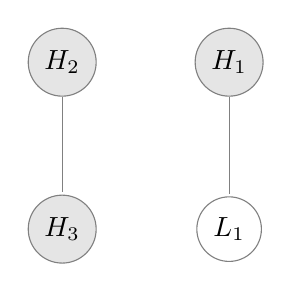
\begin{tikzpicture}[shorten >=1pt,draw=black!50]
	\node (H1) at ( 1.06,  1.06)	[circle, draw, fill = gray!20]	{$H_{1}$};
	\node (H2) at (-1.06,  1.06)	[circle, draw, fill = gray!20]	{$H_{2}$};
	\node (H3) at (-1.06, -1.06)	[circle, draw, fill = gray!20]	{$H_{3}$};
	\node (L1) at ( 1.06, -1.06)	[circle, draw, fill = white]	{$L_{1}$};
	\draw (H1) -- (L1);
	\draw (H2) -- (H3);
\end{tikzpicture}
\end{center}
\columnbreak

\scaleeq{
Equations: \begin{cases}
	e^{H}_{1} \left(\frac{25 \phi}{3} - 3\right) = \alpha - 2 e^{H}_{2} - 2 e^{H}_{3} + 3 e^{L}_{1} \theta - \gamma\\
	e^{H}_{2} \left(\frac{25 \phi}{3} - 3\right) = \alpha - 2 e^{H}_{1} + 3 e^{H}_{3} - 2 e^{L}_{1} \theta - \gamma\\
	e^{H}_{3} \left(\frac{25 \phi}{3} - 3\right) = \alpha - 2 e^{H}_{1} + 3 e^{H}_{2} - 2 e^{L}_{1} \theta - \gamma\\
	e^{L}_{1} \left(\frac{25 \phi}{3 \theta} - 3 \theta\right) = \alpha + 3 e^{H}_{1} - 2 e^{H}_{2} - 2 e^{H}_{3} - \gamma
\end{cases}
}\end{multicols}


Optimal efforts:

\scaleeq{
\begin{cases}
	e^{H}_{1} &= \frac{3 \left(\alpha - \gamma\right) \left(5 \phi - 6\right)}{125 \phi^{2} - 45 \phi \theta^{2} - 135 \phi + 18 \theta^{2} + 18}\\
	e^{H}_{2} &= \frac{3 \left(\alpha - \gamma\right) \left(5 \phi - 3 \theta^{2} - 3\right)}{125 \phi^{2} - 45 \phi \theta^{2} - 135 \phi + 18 \theta^{2} + 18}\\
	e^{H}_{3} &= \frac{3 \left(\alpha - \gamma\right) \left(5 \phi - 3 \theta^{2} - 3\right)}{125 \phi^{2} - 45 \phi \theta^{2} - 135 \phi + 18 \theta^{2} + 18}\\
	e^{L}_{1} &= \frac{3 \theta \left(\alpha - \gamma\right) \left(5 \phi - 6\right)}{125 \phi^{2} - 45 \phi \theta^{2} - 135 \phi + 18 \theta^{2} + 18}
\end{cases}
}

Production Costs:

\scaleeq{
\begin{cases}
	c^{H}_{1} &= - \frac{15 \alpha \phi \theta^{2} + 15 \alpha \phi - 18 \alpha \theta^{2} - 18 \alpha - 125 \gamma \phi^{2} + 30 \gamma \phi \theta^{2} + 120 \gamma \phi}{125 \phi^{2} - 45 \phi \theta^{2} - 135 \phi + 18 \theta^{2} + 18}\\
	c^{H}_{2} &= - \frac{30 \alpha \phi - 18 \alpha \theta^{2} - 18 \alpha - 125 \gamma \phi^{2} + 45 \gamma \phi \theta^{2} + 105 \gamma \phi}{125 \phi^{2} - 45 \phi \theta^{2} - 135 \phi + 18 \theta^{2} + 18}\\
	c^{H}_{3} &= - \frac{30 \alpha \phi - 18 \alpha \theta^{2} - 18 \alpha - 125 \gamma \phi^{2} + 45 \gamma \phi \theta^{2} + 105 \gamma \phi}{125 \phi^{2} - 45 \phi \theta^{2} - 135 \phi + 18 \theta^{2} + 18}\\
	c^{L}_{1} &= - \frac{15 \alpha \phi \theta^{2} + 15 \alpha \phi - 18 \alpha \theta^{2} - 18 \alpha - 125 \gamma \phi^{2} + 30 \gamma \phi \theta^{2} + 120 \gamma \phi}{125 \phi^{2} - 45 \phi \theta^{2} - 135 \phi + 18 \theta^{2} + 18}
\end{cases}
}

Production Quantities:

\scaleeq{
\begin{cases}
	q^{H}_{1} &= \frac{5 \phi \left(\alpha - \gamma\right) \left(5 \phi - 6\right)}{125 \phi^{2} - 45 \phi \theta^{2} - 135 \phi + 18 \theta^{2} + 18}\\
	q^{H}_{2} &= \frac{5 \phi \left(\alpha - \gamma\right) \left(5 \phi - 3 \theta^{2} - 3\right)}{125 \phi^{2} - 45 \phi \theta^{2} - 135 \phi + 18 \theta^{2} + 18}\\
	q^{H}_{3} &= \frac{5 \phi \left(\alpha - \gamma\right) \left(5 \phi - 3 \theta^{2} - 3\right)}{125 \phi^{2} - 45 \phi \theta^{2} - 135 \phi + 18 \theta^{2} + 18}\\
	q^{L}_{1} &= \frac{5 \phi \left(\alpha - \gamma\right) \left(5 \phi - 6\right)}{125 \phi^{2} - 45 \phi \theta^{2} - 135 \phi + 18 \theta^{2} + 18}
\end{cases}
}

Profits:

\begin{equation}
\label{eq:E2C:3H1L_profit}
\scaledequation{\begin{cases}
	\pi^{H}_{1} &= \frac{\phi \left(\alpha - \gamma\right)^{2} \left(5 \phi - 6\right)^{2} \left(25 \phi - 9\right)}{\left(125 \phi^{2} - 45 \phi \theta^{2} - 135 \phi + 18 \theta^{2} + 18\right)^{2}}\\
	\pi^{H}_{2} &= \frac{\phi \left(\alpha - \gamma\right)^{2} \left(25 \phi - 9\right) \left(5 \phi - 3 \theta^{2} - 3\right)^{2}}{\left(125 \phi^{2} - 45 \phi \theta^{2} - 135 \phi + 18 \theta^{2} + 18\right)^{2}}\\
	\pi^{H}_{3} &= \frac{\phi \left(\alpha - \gamma\right)^{2} \left(25 \phi - 9\right) \left(5 \phi - 3 \theta^{2} - 3\right)^{2}}{\left(125 \phi^{2} - 45 \phi \theta^{2} - 135 \phi + 18 \theta^{2} + 18\right)^{2}}\\
	\pi^{L}_{1} &= \frac{\phi \left(\alpha - \gamma\right)^{2} \left(5 \phi - 6\right)^{2} \left(25 \phi - 9 \theta^{2}\right)}{\left(125 \phi^{2} - 45 \phi \theta^{2} - 135 \phi + 18 \theta^{2} + 18\right)^{2}}
\end{cases}
}
\end{equation}

Total Production:

\scaleeq{
\frac{10 \phi \left(\alpha - \gamma\right) \left(10 \phi - 3 \theta^{2} - 9\right)}{125 \phi^{2} - 45 \phi \theta^{2} - 135 \phi + 18 \theta^{2} + 18}
}

Price:

\scaleeq{
\frac{25 \alpha \phi^{2} - 15 \alpha \phi \theta^{2} - 45 \alpha \phi + 18 \alpha \theta^{2} + 18 \alpha + 100 \gamma \phi^{2} - 30 \gamma \phi \theta^{2} - 90 \gamma \phi}{125 \phi^{2} - 45 \phi \theta^{2} - 135 \phi + 18 \theta^{2} + 18}
}

Firm Surplus:

\scaleeq{
\frac{\phi \left(\alpha - \gamma\right)^{2} \left(2500 \phi^{3} - 1725 \phi^{2} \theta^{2} - 5175 \phi^{2} + 450 \phi \theta^{4} + 1980 \phi \theta^{2} + 3330 \phi - 162 \theta^{4} - 648 \theta^{2} - 486\right)}{\left(125 \phi^{2} - 45 \phi \theta^{2} - 135 \phi + 18 \theta^{2} + 18\right)^{2}}
}

Consumer Surplus:

\scaleeq{
\frac{50 \phi^{2} \left(\alpha - \gamma\right)^{2} \left(10 \phi - 3 \theta^{2} - 9\right)^{2}}{\left(125 \phi^{2} - 45 \phi \theta^{2} - 135 \phi + 18 \theta^{2} + 18\right)^{2}}
}

Social Welfare:

\scaleeq{
\frac{3 \phi \left(\alpha - \gamma\right)^{2} \left(2500 \phi^{3} - 1575 \phi^{2} \theta^{2} - 4725 \phi^{2} + 300 \phi \theta^{4} + 1560 \phi \theta^{2} + 2460 \phi - 54 \theta^{4} - 216 \theta^{2} - 162\right)}{\left(125 \phi^{2} - 45 \phi \theta^{2} - 135 \phi + 18 \theta^{2} + 18\right)^{2}}
}

%======================================================================

\subsubsection{E2D [3H1L]}
\label{apx:E2D:3H1L}

\begin{multicols}{2}
\begin{center}
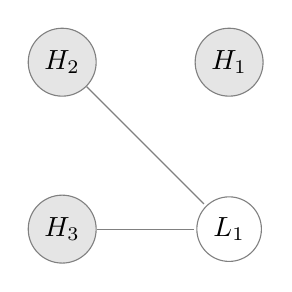
\begin{tikzpicture}[shorten >=1pt,draw=black!50]
	\node (H1) at ( 1.06,  1.06)	[circle, draw, fill = gray!20]	{$H_{1}$};
	\node (H2) at (-1.06,  1.06)	[circle, draw, fill = gray!20]	{$H_{2}$};
	\node (H3) at (-1.06, -1.06)	[circle, draw, fill = gray!20]	{$H_{3}$};
	\node (L1) at ( 1.06, -1.06)	[circle, draw, fill = white]	{$L_{1}$};
	\draw (H2) -- (L1);
	\draw (H3) -- (L1);
\end{tikzpicture}
\end{center}
\columnbreak

\scaleeq{
Equations: \begin{cases}
	e^{H}_{1} \left(\frac{25 \phi}{4} - 4\right) = \alpha - 2 e^{H}_{2} - 2 e^{H}_{3} - 3 e^{L}_{1} \theta - \gamma\\
	e^{H}_{2} \left(\frac{25 \phi}{3} - 3\right) = \alpha - e^{H}_{1} - 2 e^{H}_{3} + 2 e^{L}_{1} \theta - \gamma\\
	e^{H}_{3} \left(\frac{25 \phi}{3} - 3\right) = \alpha - e^{H}_{1} - 2 e^{H}_{2} + 2 e^{L}_{1} \theta - \gamma\\
	e^{L}_{1} \left(\frac{25 \phi}{2 \theta} - 2 \theta\right) = \alpha - e^{H}_{1} + 3 e^{H}_{2} + 3 e^{H}_{3} - \gamma
\end{cases}
}\end{multicols}


Optimal efforts:

\scaleeq{
\begin{cases}
	e^{H}_{1} &= \frac{4 \left(\alpha - \gamma\right) \left(25 \phi^{2} - 10 \phi \theta^{2} - 15 \phi - 6 \theta^{2}\right)}{625 \phi^{3} - 100 \phi^{2} \theta^{2} - 475 \phi^{2} - 20 \phi \theta^{2} + 24 \theta^{2}}\\
	e^{H}_{2} &= \frac{15 \phi \left(\alpha - \gamma\right) \left(5 \phi - 4\right)}{625 \phi^{3} - 100 \phi^{2} \theta^{2} - 475 \phi^{2} - 20 \phi \theta^{2} + 24 \theta^{2}}\\
	e^{H}_{3} &= \frac{15 \phi \left(\alpha - \gamma\right) \left(5 \phi - 4\right)}{625 \phi^{3} - 100 \phi^{2} \theta^{2} - 475 \phi^{2} - 20 \phi \theta^{2} + 24 \theta^{2}}\\
	e^{L}_{1} &= \frac{2 \theta \left(\alpha - \gamma\right) \left(5 \phi - 4\right) \left(5 \phi + 3\right)}{625 \phi^{3} - 100 \phi^{2} \theta^{2} - 475 \phi^{2} - 20 \phi \theta^{2} + 24 \theta^{2}}
\end{cases}
}

Production Costs:

\scaleeq{
\begin{cases}
	c^{H}_{1} &= - \frac{100 \alpha \phi^{2} - 40 \alpha \phi \theta^{2} - 60 \alpha \phi - 24 \alpha \theta^{2} - 625 \gamma \phi^{3} + 100 \gamma \phi^{2} \theta^{2} + 375 \gamma \phi^{2} + 60 \gamma \phi \theta^{2} + 60 \gamma \phi}{625 \phi^{3} - 100 \phi^{2} \theta^{2} - 475 \phi^{2} - 20 \phi \theta^{2} + 24 \theta^{2}}\\
	c^{H}_{2} &= - \frac{50 \alpha \phi^{2} \theta^{2} + 75 \alpha \phi^{2} - 10 \alpha \phi \theta^{2} - 60 \alpha \phi - 24 \alpha \theta^{2} - 625 \gamma \phi^{3} + 50 \gamma \phi^{2} \theta^{2} + 400 \gamma \phi^{2} + 30 \gamma \phi \theta^{2} + 60 \gamma \phi}{625 \phi^{3} - 100 \phi^{2} \theta^{2} - 475 \phi^{2} - 20 \phi \theta^{2} + 24 \theta^{2}}\\
	c^{H}_{3} &= - \frac{50 \alpha \phi^{2} \theta^{2} + 75 \alpha \phi^{2} - 10 \alpha \phi \theta^{2} - 60 \alpha \phi - 24 \alpha \theta^{2} - 625 \gamma \phi^{3} + 50 \gamma \phi^{2} \theta^{2} + 400 \gamma \phi^{2} + 30 \gamma \phi \theta^{2} + 60 \gamma \phi}{625 \phi^{3} - 100 \phi^{2} \theta^{2} - 475 \phi^{2} - 20 \phi \theta^{2} + 24 \theta^{2}}\\
	c^{L}_{1} &= - \frac{50 \alpha \phi^{2} \theta^{2} + 150 \alpha \phi^{2} - 10 \alpha \phi \theta^{2} - 120 \alpha \phi - 24 \alpha \theta^{2} - 625 \gamma \phi^{3} + 50 \gamma \phi^{2} \theta^{2} + 325 \gamma \phi^{2} + 30 \gamma \phi \theta^{2} + 120 \gamma \phi}{625 \phi^{3} - 100 \phi^{2} \theta^{2} - 475 \phi^{2} - 20 \phi \theta^{2} + 24 \theta^{2}}
\end{cases}
}

Production Quantities:

\scaleeq{
\begin{cases}
	q^{H}_{1} &= \frac{5 \phi \left(\alpha - \gamma\right) \left(25 \phi^{2} - 10 \phi \theta^{2} - 15 \phi - 6 \theta^{2}\right)}{625 \phi^{3} - 100 \phi^{2} \theta^{2} - 475 \phi^{2} - 20 \phi \theta^{2} + 24 \theta^{2}}\\
	q^{H}_{2} &= \frac{25 \phi^{2} \left(\alpha - \gamma\right) \left(5 \phi - 4\right)}{625 \phi^{3} - 100 \phi^{2} \theta^{2} - 475 \phi^{2} - 20 \phi \theta^{2} + 24 \theta^{2}}\\
	q^{H}_{3} &= \frac{25 \phi^{2} \left(\alpha - \gamma\right) \left(5 \phi - 4\right)}{625 \phi^{3} - 100 \phi^{2} \theta^{2} - 475 \phi^{2} - 20 \phi \theta^{2} + 24 \theta^{2}}\\
	q^{L}_{1} &= \frac{5 \phi \left(\alpha - \gamma\right) \left(5 \phi - 4\right) \left(5 \phi + 3\right)}{625 \phi^{3} - 100 \phi^{2} \theta^{2} - 475 \phi^{2} - 20 \phi \theta^{2} + 24 \theta^{2}}
\end{cases}
}

Profits:

\begin{equation}
\label{eq:E2D:3H1L_profit}
\scaledequation{\begin{cases}
	\pi^{H}_{1} &= \frac{\phi \left(\alpha - \gamma\right)^{2} \left(25 \phi - 16\right) \left(25 \phi^{2} - 10 \phi \theta^{2} - 15 \phi - 6 \theta^{2}\right)^{2}}{\left(625 \phi^{3} - 100 \phi^{2} \theta^{2} - 475 \phi^{2} - 20 \phi \theta^{2} + 24 \theta^{2}\right)^{2}}\\
	\pi^{H}_{2} &= \frac{25 \phi^{3} \left(\alpha - \gamma\right)^{2} \left(5 \phi - 4\right)^{2} \left(25 \phi - 9\right)}{\left(625 \phi^{3} - 100 \phi^{2} \theta^{2} - 475 \phi^{2} - 20 \phi \theta^{2} + 24 \theta^{2}\right)^{2}}\\
	\pi^{H}_{3} &= \frac{25 \phi^{3} \left(\alpha - \gamma\right)^{2} \left(5 \phi - 4\right)^{2} \left(25 \phi - 9\right)}{\left(625 \phi^{3} - 100 \phi^{2} \theta^{2} - 475 \phi^{2} - 20 \phi \theta^{2} + 24 \theta^{2}\right)^{2}}\\
	\pi^{L}_{1} &= \frac{\phi \left(\alpha - \gamma\right)^{2} \left(5 \phi - 4\right)^{2} \left(5 \phi + 3\right)^{2} \left(25 \phi - 4 \theta^{2}\right)}{\left(625 \phi^{3} - 100 \phi^{2} \theta^{2} - 475 \phi^{2} - 20 \phi \theta^{2} + 24 \theta^{2}\right)^{2}}
\end{cases}
}
\end{equation}

Total Production:

\scaleeq{
\frac{10 \phi \left(\alpha - \gamma\right) \left(50 \phi^{2} - 5 \phi \theta^{2} - 30 \phi - 3 \theta^{2} - 6\right)}{625 \phi^{3} - 100 \phi^{2} \theta^{2} - 475 \phi^{2} - 20 \phi \theta^{2} + 24 \theta^{2}}
}

Price:

\scaleeq{
\frac{125 \alpha \phi^{3} - 50 \alpha \phi^{2} \theta^{2} - 175 \alpha \phi^{2} + 10 \alpha \phi \theta^{2} + 60 \alpha \phi + 24 \alpha \theta^{2} + 500 \gamma \phi^{3} - 50 \gamma \phi^{2} \theta^{2} - 300 \gamma \phi^{2} - 30 \gamma \phi \theta^{2} - 60 \gamma \phi}{625 \phi^{3} - 100 \phi^{2} \theta^{2} - 475 \phi^{2} - 20 \phi \theta^{2} + 24 \theta^{2}}
}

Firm Surplus:

\scaleeq{
\frac{2 \phi \left(\alpha - \gamma\right)^{2} \left(31250 \phi^{5} - 7500 \phi^{4} \theta^{2} - 48125 \phi^{4} + 1250 \phi^{3} \theta^{4} + 4500 \phi^{3} \theta^{2} + 20625 \phi^{3} + 700 \phi^{2} \theta^{4} + 3400 \phi^{2} \theta^{2} - 3900 \phi^{2} - 510 \phi \theta^{4} - 1680 \phi \theta^{2} + 1800 \phi - 288 \theta^{4} - 288 \theta^{2}\right)}{\left(625 \phi^{3} - 100 \phi^{2} \theta^{2} - 475 \phi^{2} - 20 \phi \theta^{2} + 24 \theta^{2}\right)^{2}}
}

Consumer Surplus:

\scaleeq{
\frac{50 \phi^{2} \left(\alpha - \gamma\right)^{2} \left(50 \phi^{2} - 5 \phi \theta^{2} - 30 \phi - 3 \theta^{2} - 6\right)^{2}}{\left(625 \phi^{3} - 100 \phi^{2} \theta^{2} - 475 \phi^{2} - 20 \phi \theta^{2} + 24 \theta^{2}\right)^{2}}
}

Social Welfare:

\scaleeq{
\frac{2 \phi \left(\alpha - \gamma\right)^{2} \left(93750 \phi^{5} - 20000 \phi^{4} \theta^{2} - 123125 \phi^{4} + 1875 \phi^{3} \theta^{4} + 4500 \phi^{3} \theta^{2} + 28125 \phi^{3} + 1450 \phi^{2} \theta^{4} + 9400 \phi^{2} \theta^{2} + 5100 \phi^{2} - 285 \phi \theta^{4} - 780 \phi \theta^{2} + 2700 \phi - 288 \theta^{4} - 288 \theta^{2}\right)}{\left(625 \phi^{3} - 100 \phi^{2} \theta^{2} - 475 \phi^{2} - 20 \phi \theta^{2} + 24 \theta^{2}\right)^{2}}
}

%======================================================================

\subsubsection{E3A [3H1L]}
\label{apx:E3A:3H1L}

\begin{multicols}{2}
\begin{center}
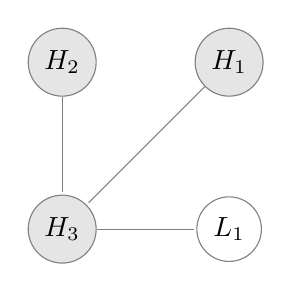
\begin{tikzpicture}[shorten >=1pt,draw=black!50]
	\node (H1) at ( 1.06,  1.06)	[circle, draw, fill = gray!20]	{$H_{1}$};
	\node (H2) at (-1.06,  1.06)	[circle, draw, fill = gray!20]	{$H_{2}$};
	\node (H3) at (-1.06, -1.06)	[circle, draw, fill = gray!20]	{$H_{3}$};
	\node (L1) at ( 1.06, -1.06)	[circle, draw, fill = white]	{$L_{1}$};
	\draw (H1) -- (H3);
	\draw (H2) -- (H3);
	\draw (H3) -- (L1);
\end{tikzpicture}
\end{center}
\columnbreak

\scaleeq{
Equations: \begin{cases}
	e^{H}_{1} \left(\frac{25 \phi}{3} - 3\right) = \alpha - 2 e^{H}_{2} + e^{H}_{3} - 2 e^{L}_{1} \theta - \gamma\\
	e^{H}_{2} \left(\frac{25 \phi}{3} - 3\right) = \alpha - 2 e^{H}_{1} + e^{H}_{3} - 2 e^{L}_{1} \theta - \gamma\\
	e^{H}_{3} \left(25 \phi - 1\right) = \alpha + 3 e^{H}_{1} + 3 e^{H}_{2} + 3 e^{L}_{1} \theta - \gamma\\
	e^{L}_{1} \left(\frac{25 \phi}{3 \theta} - 3 \theta\right) = \alpha - 2 e^{H}_{1} - 2 e^{H}_{2} + e^{H}_{3} - \gamma
\end{cases}
}\end{multicols}


Optimal efforts:

\scaleeq{
\begin{cases}
	e^{H}_{1} &= \frac{15 \phi \left(\alpha - \gamma\right) \left(5 \phi - 3 \theta^{2}\right)}{625 \phi^{3} - 225 \phi^{2} \theta^{2} - 100 \phi^{2} - 45 \phi \theta^{2} - 15 \phi + 18 \theta^{2}}\\
	e^{H}_{2} &= \frac{15 \phi \left(\alpha - \gamma\right) \left(5 \phi - 3 \theta^{2}\right)}{625 \phi^{3} - 225 \phi^{2} \theta^{2} - 100 \phi^{2} - 45 \phi \theta^{2} - 15 \phi + 18 \theta^{2}}\\
	e^{H}_{3} &= \frac{\left(\alpha - \gamma\right) \left(25 \phi^{2} + 15 \phi - 18 \theta^{2}\right)}{625 \phi^{3} - 225 \phi^{2} \theta^{2} - 100 \phi^{2} - 45 \phi \theta^{2} - 15 \phi + 18 \theta^{2}}\\
	e^{L}_{1} &= \frac{15 \phi \theta \left(\alpha - \gamma\right) \left(5 \phi - 3\right)}{625 \phi^{3} - 225 \phi^{2} \theta^{2} - 100 \phi^{2} - 45 \phi \theta^{2} - 15 \phi + 18 \theta^{2}}
\end{cases}
}

Production Costs:

\scaleeq{
\begin{cases}
	c^{H}_{1} &= - \frac{100 \alpha \phi^{2} - 45 \alpha \phi \theta^{2} + 15 \alpha \phi - 18 \alpha \theta^{2} - 625 \gamma \phi^{3} + 225 \gamma \phi^{2} \theta^{2} + 90 \gamma \phi \theta^{2}}{625 \phi^{3} - 225 \phi^{2} \theta^{2} - 100 \phi^{2} - 45 \phi \theta^{2} - 15 \phi + 18 \theta^{2}}\\
	c^{H}_{2} &= - \frac{100 \alpha \phi^{2} - 45 \alpha \phi \theta^{2} + 15 \alpha \phi - 18 \alpha \theta^{2} - 625 \gamma \phi^{3} + 225 \gamma \phi^{2} \theta^{2} + 90 \gamma \phi \theta^{2}}{625 \phi^{3} - 225 \phi^{2} \theta^{2} - 100 \phi^{2} - 45 \phi \theta^{2} - 15 \phi + 18 \theta^{2}}\\
	c^{H}_{3} &= - \frac{75 \alpha \phi^{2} \theta^{2} + 175 \alpha \phi^{2} - 135 \alpha \phi \theta^{2} + 15 \alpha \phi - 18 \alpha \theta^{2} - 625 \gamma \phi^{3} + 150 \gamma \phi^{2} \theta^{2} - 75 \gamma \phi^{2} + 180 \gamma \phi \theta^{2}}{625 \phi^{3} - 225 \phi^{2} \theta^{2} - 100 \phi^{2} - 45 \phi \theta^{2} - 15 \phi + 18 \theta^{2}}\\
	c^{L}_{1} &= - \frac{75 \alpha \phi^{2} \theta^{2} + 25 \alpha \phi^{2} - 45 \alpha \phi \theta^{2} + 15 \alpha \phi - 18 \alpha \theta^{2} - 625 \gamma \phi^{3} + 150 \gamma \phi^{2} \theta^{2} + 75 \gamma \phi^{2} + 90 \gamma \phi \theta^{2}}{625 \phi^{3} - 225 \phi^{2} \theta^{2} - 100 \phi^{2} - 45 \phi \theta^{2} - 15 \phi + 18 \theta^{2}}
\end{cases}
}

Production Quantities:

\scaleeq{
\begin{cases}
	q^{H}_{1} &= \frac{25 \phi^{2} \left(\alpha - \gamma\right) \left(5 \phi - 3 \theta^{2}\right)}{625 \phi^{3} - 225 \phi^{2} \theta^{2} - 100 \phi^{2} - 45 \phi \theta^{2} - 15 \phi + 18 \theta^{2}}\\
	q^{H}_{2} &= \frac{25 \phi^{2} \left(\alpha - \gamma\right) \left(5 \phi - 3 \theta^{2}\right)}{625 \phi^{3} - 225 \phi^{2} \theta^{2} - 100 \phi^{2} - 45 \phi \theta^{2} - 15 \phi + 18 \theta^{2}}\\
	q^{H}_{3} &= \frac{5 \phi \left(\alpha - \gamma\right) \left(25 \phi^{2} + 15 \phi - 18 \theta^{2}\right)}{625 \phi^{3} - 225 \phi^{2} \theta^{2} - 100 \phi^{2} - 45 \phi \theta^{2} - 15 \phi + 18 \theta^{2}}\\
	q^{L}_{1} &= \frac{25 \phi^{2} \left(\alpha - \gamma\right) \left(5 \phi - 3\right)}{625 \phi^{3} - 225 \phi^{2} \theta^{2} - 100 \phi^{2} - 45 \phi \theta^{2} - 15 \phi + 18 \theta^{2}}
\end{cases}
}

Profits:

\begin{equation}
\label{eq:E3A:3H1L_profit}
\scaledequation{\begin{cases}
	\pi^{H}_{1} &= \frac{25 \phi^{3} \left(\alpha - \gamma\right)^{2} \left(5 \phi - 3 \theta^{2}\right)^{2} \left(25 \phi - 9\right)}{\left(625 \phi^{3} - 225 \phi^{2} \theta^{2} - 100 \phi^{2} - 45 \phi \theta^{2} - 15 \phi + 18 \theta^{2}\right)^{2}}\\
	\pi^{H}_{2} &= \frac{25 \phi^{3} \left(\alpha - \gamma\right)^{2} \left(5 \phi - 3 \theta^{2}\right)^{2} \left(25 \phi - 9\right)}{\left(625 \phi^{3} - 225 \phi^{2} \theta^{2} - 100 \phi^{2} - 45 \phi \theta^{2} - 15 \phi + 18 \theta^{2}\right)^{2}}\\
	\pi^{H}_{3} &= \frac{\phi \left(\alpha - \gamma\right)^{2} \left(25 \phi - 1\right) \left(25 \phi^{2} + 15 \phi - 18 \theta^{2}\right)^{2}}{\left(625 \phi^{3} - 225 \phi^{2} \theta^{2} - 100 \phi^{2} - 45 \phi \theta^{2} - 15 \phi + 18 \theta^{2}\right)^{2}}\\
	\pi^{L}_{1} &= \frac{25 \phi^{3} \left(\alpha - \gamma\right)^{2} \left(5 \phi - 3\right)^{2} \left(25 \phi - 9 \theta^{2}\right)}{\left(625 \phi^{3} - 225 \phi^{2} \theta^{2} - 100 \phi^{2} - 45 \phi \theta^{2} - 15 \phi + 18 \theta^{2}\right)^{2}}
\end{cases}
}
\end{equation}

Total Production:

\scaleeq{
\frac{10 \phi \left(\alpha - \gamma\right) \left(50 \phi^{2} - 15 \phi \theta^{2} - 9 \theta^{2}\right)}{625 \phi^{3} - 225 \phi^{2} \theta^{2} - 100 \phi^{2} - 45 \phi \theta^{2} - 15 \phi + 18 \theta^{2}}
}

Price:

\scaleeq{
\frac{125 \alpha \phi^{3} - 75 \alpha \phi^{2} \theta^{2} - 100 \alpha \phi^{2} + 45 \alpha \phi \theta^{2} - 15 \alpha \phi + 18 \alpha \theta^{2} + 500 \gamma \phi^{3} - 150 \gamma \phi^{2} \theta^{2} - 90 \gamma \phi \theta^{2}}{625 \phi^{3} - 225 \phi^{2} \theta^{2} - 100 \phi^{2} - 45 \phi \theta^{2} - 15 \phi + 18 \theta^{2}}
}

Firm Surplus:

\scaleeq{
\frac{\phi \left(\alpha - \gamma\right)^{2} \left(62500 \phi^{5} - 43125 \phi^{4} \theta^{2} - 11875 \phi^{4} + 11250 \phi^{3} \theta^{4} - 2250 \phi^{3} \theta^{2} + 10500 \phi^{3} - 4050 \phi^{2} \theta^{4} - 14625 \phi^{2} \theta^{2} - 225 \phi^{2} + 8100 \phi \theta^{4} + 540 \phi \theta^{2} - 324 \theta^{4}\right)}{\left(625 \phi^{3} - 225 \phi^{2} \theta^{2} - 100 \phi^{2} - 45 \phi \theta^{2} - 15 \phi + 18 \theta^{2}\right)^{2}}
}

Consumer Surplus:

\scaleeq{
\frac{50 \phi^{2} \left(\alpha - \gamma\right)^{2} \left(50 \phi^{2} - 15 \phi \theta^{2} - 9 \theta^{2}\right)^{2}}{\left(625 \phi^{3} - 225 \phi^{2} \theta^{2} - 100 \phi^{2} - 45 \phi \theta^{2} - 15 \phi + 18 \theta^{2}\right)^{2}}
}

Social Welfare:

\scaleeq{
\frac{\phi \left(\alpha - \gamma\right)^{2} \left(187500 \phi^{5} - 118125 \phi^{4} \theta^{2} - 11875 \phi^{4} + 22500 \phi^{3} \theta^{4} - 47250 \phi^{3} \theta^{2} + 10500 \phi^{3} + 9450 \phi^{2} \theta^{4} - 14625 \phi^{2} \theta^{2} - 225 \phi^{2} + 12150 \phi \theta^{4} + 540 \phi \theta^{2} - 324 \theta^{4}\right)}{\left(625 \phi^{3} - 225 \phi^{2} \theta^{2} - 100 \phi^{2} - 45 \phi \theta^{2} - 15 \phi + 18 \theta^{2}\right)^{2}}
}

%======================================================================

\subsubsection{E3B [3H1L]}
\label{apx:E3B:3H1L}

\begin{multicols}{2}
\begin{center}
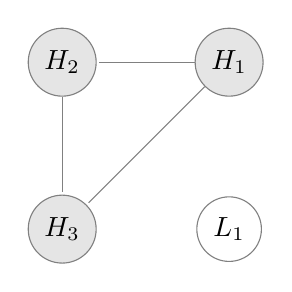
\begin{tikzpicture}[shorten >=1pt,draw=black!50]
	\node (H1) at ( 1.06,  1.06)	[circle, draw, fill = gray!20]	{$H_{1}$};
	\node (H2) at (-1.06,  1.06)	[circle, draw, fill = gray!20]	{$H_{2}$};
	\node (H3) at (-1.06, -1.06)	[circle, draw, fill = gray!20]	{$H_{3}$};
	\node (L1) at ( 1.06, -1.06)	[circle, draw, fill = white]	{$L_{1}$};
	\draw (H1) -- (H2);
	\draw (H1) -- (H3);
	\draw (H2) -- (H3);
\end{tikzpicture}
\end{center}
\columnbreak

\scaleeq{
Equations: \begin{cases}
	e^{H}_{1} \left(\frac{25 \phi}{2} - 2\right) = \alpha + 2 e^{H}_{2} + 2 e^{H}_{3} - e^{L}_{1} \theta - \gamma\\
	e^{H}_{2} \left(\frac{25 \phi}{2} - 2\right) = \alpha + 2 e^{H}_{1} + 2 e^{H}_{3} - e^{L}_{1} \theta - \gamma\\
	e^{H}_{3} \left(\frac{25 \phi}{2} - 2\right) = \alpha + 2 e^{H}_{1} + 2 e^{H}_{2} - e^{L}_{1} \theta - \gamma\\
	e^{L}_{1} \left(\frac{25 \phi}{4 \theta} - 4 \theta\right) = \alpha - 3 e^{H}_{1} - 3 e^{H}_{2} - 3 e^{H}_{3} - \gamma
\end{cases}
}\end{multicols}


Optimal efforts:

\scaleeq{
\begin{cases}
	e^{H}_{1} &= \frac{2 \left(\alpha - \gamma\right) \left(5 \phi - 4 \theta^{2}\right)}{125 \phi^{2} - 80 \phi \theta^{2} - 60 \phi + 24 \theta^{2}}\\
	e^{H}_{2} &= \frac{2 \left(\alpha - \gamma\right) \left(5 \phi - 4 \theta^{2}\right)}{125 \phi^{2} - 80 \phi \theta^{2} - 60 \phi + 24 \theta^{2}}\\
	e^{H}_{3} &= \frac{2 \left(\alpha - \gamma\right) \left(5 \phi - 4 \theta^{2}\right)}{125 \phi^{2} - 80 \phi \theta^{2} - 60 \phi + 24 \theta^{2}}\\
	e^{L}_{1} &= \frac{4 \theta \left(\alpha - \gamma\right) \left(5 \phi - 6\right)}{125 \phi^{2} - 80 \phi \theta^{2} - 60 \phi + 24 \theta^{2}}
\end{cases}
}

Production Costs:

\scaleeq{
\begin{cases}
	c^{H}_{1} &= - \frac{30 \alpha \phi - 24 \alpha \theta^{2} - 125 \gamma \phi^{2} + 80 \gamma \phi \theta^{2} + 30 \gamma \phi}{125 \phi^{2} - 80 \phi \theta^{2} - 60 \phi + 24 \theta^{2}}\\
	c^{H}_{2} &= - \frac{30 \alpha \phi - 24 \alpha \theta^{2} - 125 \gamma \phi^{2} + 80 \gamma \phi \theta^{2} + 30 \gamma \phi}{125 \phi^{2} - 80 \phi \theta^{2} - 60 \phi + 24 \theta^{2}}\\
	c^{H}_{3} &= - \frac{30 \alpha \phi - 24 \alpha \theta^{2} - 125 \gamma \phi^{2} + 80 \gamma \phi \theta^{2} + 30 \gamma \phi}{125 \phi^{2} - 80 \phi \theta^{2} - 60 \phi + 24 \theta^{2}}\\
	c^{L}_{1} &= - \frac{20 \alpha \phi \theta^{2} - 24 \alpha \theta^{2} - 125 \gamma \phi^{2} + 60 \gamma \phi \theta^{2} + 60 \gamma \phi}{125 \phi^{2} - 80 \phi \theta^{2} - 60 \phi + 24 \theta^{2}}
\end{cases}
}

Production Quantities:

\scaleeq{
\begin{cases}
	q^{H}_{1} &= \frac{5 \phi \left(\alpha - \gamma\right) \left(5 \phi - 4 \theta^{2}\right)}{125 \phi^{2} - 80 \phi \theta^{2} - 60 \phi + 24 \theta^{2}}\\
	q^{H}_{2} &= \frac{5 \phi \left(\alpha - \gamma\right) \left(5 \phi - 4 \theta^{2}\right)}{125 \phi^{2} - 80 \phi \theta^{2} - 60 \phi + 24 \theta^{2}}\\
	q^{H}_{3} &= \frac{5 \phi \left(\alpha - \gamma\right) \left(5 \phi - 4 \theta^{2}\right)}{125 \phi^{2} - 80 \phi \theta^{2} - 60 \phi + 24 \theta^{2}}\\
	q^{L}_{1} &= \frac{5 \phi \left(\alpha - \gamma\right) \left(5 \phi - 6\right)}{125 \phi^{2} - 80 \phi \theta^{2} - 60 \phi + 24 \theta^{2}}
\end{cases}
}

Profits:

\begin{equation}
\label{eq:E3B:3H1L_profit}
\scaledequation{\begin{cases}
	\pi^{H}_{1} &= \frac{\phi \left(\alpha - \gamma\right)^{2} \left(5 \phi - 4 \theta^{2}\right)^{2} \left(25 \phi - 4\right)}{\left(125 \phi^{2} - 80 \phi \theta^{2} - 60 \phi + 24 \theta^{2}\right)^{2}}\\
	\pi^{H}_{2} &= \frac{\phi \left(\alpha - \gamma\right)^{2} \left(5 \phi - 4 \theta^{2}\right)^{2} \left(25 \phi - 4\right)}{\left(125 \phi^{2} - 80 \phi \theta^{2} - 60 \phi + 24 \theta^{2}\right)^{2}}\\
	\pi^{H}_{3} &= \frac{\phi \left(\alpha - \gamma\right)^{2} \left(5 \phi - 4 \theta^{2}\right)^{2} \left(25 \phi - 4\right)}{\left(125 \phi^{2} - 80 \phi \theta^{2} - 60 \phi + 24 \theta^{2}\right)^{2}}\\
	\pi^{L}_{1} &= \frac{\phi \left(\alpha - \gamma\right)^{2} \left(5 \phi - 6\right)^{2} \left(25 \phi - 16 \theta^{2}\right)}{\left(125 \phi^{2} - 80 \phi \theta^{2} - 60 \phi + 24 \theta^{2}\right)^{2}}
\end{cases}
}
\end{equation}

Total Production:

\scaleeq{
\frac{10 \phi \left(\alpha - \gamma\right) \left(10 \phi - 6 \theta^{2} - 3\right)}{125 \phi^{2} - 80 \phi \theta^{2} - 60 \phi + 24 \theta^{2}}
}

Price:

\scaleeq{
\frac{25 \alpha \phi^{2} - 20 \alpha \phi \theta^{2} - 30 \alpha \phi + 24 \alpha \theta^{2} + 100 \gamma \phi^{2} - 60 \gamma \phi \theta^{2} - 30 \gamma \phi}{125 \phi^{2} - 80 \phi \theta^{2} - 60 \phi + 24 \theta^{2}}
}

Firm Surplus:

\scaleeq{
\frac{4 \phi \left(\alpha - \gamma\right)^{2} \left(625 \phi^{3} - 850 \phi^{2} \theta^{2} - 450 \phi^{2} + 300 \phi \theta^{4} + 360 \phi \theta^{2} + 225 \phi - 48 \theta^{4} - 144 \theta^{2}\right)}{\left(125 \phi^{2} - 80 \phi \theta^{2} - 60 \phi + 24 \theta^{2}\right)^{2}}
}

Consumer Surplus:

\scaleeq{
\frac{50 \phi^{2} \left(\alpha - \gamma\right)^{2} \left(10 \phi - 6 \theta^{2} - 3\right)^{2}}{\left(125 \phi^{2} - 80 \phi \theta^{2} - 60 \phi + 24 \theta^{2}\right)^{2}}
}

Social Welfare:

\scaleeq{
\frac{2 \phi \left(\alpha - \gamma\right)^{2} \left(3750 \phi^{3} - 4700 \phi^{2} \theta^{2} - 2400 \phi^{2} + 1500 \phi \theta^{4} + 1620 \phi \theta^{2} + 675 \phi - 96 \theta^{4} - 288 \theta^{2}\right)}{\left(125 \phi^{2} - 80 \phi \theta^{2} - 60 \phi + 24 \theta^{2}\right)^{2}}
}

%======================================================================

\subsubsection{E3C [3H1L]}
\label{apx:E3C:3H1L}

\begin{multicols}{2}
\begin{center}
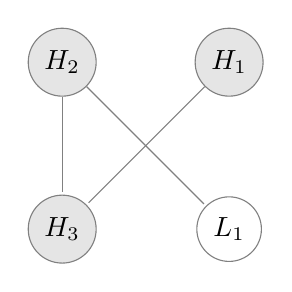
\begin{tikzpicture}[shorten >=1pt,draw=black!50]
	\node (H1) at ( 1.06,  1.06)	[circle, draw, fill = gray!20]	{$H_{1}$};
	\node (H2) at (-1.06,  1.06)	[circle, draw, fill = gray!20]	{$H_{2}$};
	\node (H3) at (-1.06, -1.06)	[circle, draw, fill = gray!20]	{$H_{3}$};
	\node (L1) at ( 1.06, -1.06)	[circle, draw, fill = white]	{$L_{1}$};
	\draw (H1) -- (H3);
	\draw (H2) -- (H3);
	\draw (H2) -- (L1);
\end{tikzpicture}
\end{center}
\columnbreak

\scaleeq{
Equations: \begin{cases}
	e^{H}_{1} \left(\frac{25 \phi}{3} - 3\right) = \alpha - 3 e^{H}_{2} + 2 e^{H}_{3} - 2 e^{L}_{1} \theta - \gamma\\
	e^{H}_{2} \left(\frac{25 \phi}{2} - 2\right) = \alpha - 2 e^{H}_{1} + 2 e^{H}_{3} + 3 e^{L}_{1} \theta - \gamma\\
	e^{H}_{3} \left(\frac{25 \phi}{2} - 2\right) = \alpha + 3 e^{H}_{1} + 2 e^{H}_{2} - 2 e^{L}_{1} \theta - \gamma\\
	e^{L}_{1} \left(\frac{25 \phi}{3 \theta} - 3 \theta\right) = \alpha - 2 e^{H}_{1} + 2 e^{H}_{2} - 3 e^{H}_{3} - \gamma
\end{cases}
}\end{multicols}


Optimal efforts:

\scaleeq{
\begin{cases}
	e^{H}_{1} &= \frac{3 \left(\alpha - \gamma\right) \left(5 \phi - 2\right) \left(25 \phi^{2} - 15 \phi \theta^{2} - 6 \theta^{2}\right)}{3125 \phi^{4} - 1125 \phi^{3} \theta^{2} - 2125 \phi^{3} + 225 \phi^{2} \theta^{2} + 120 \phi \theta^{2} + 120 \phi - 36 \theta^{2}}\\
	e^{H}_{2} &= \frac{10 \phi \left(\alpha - \gamma\right) \left(25 \phi^{2} - 15 \phi - 6 \theta^{2}\right)}{3125 \phi^{4} - 1125 \phi^{3} \theta^{2} - 2125 \phi^{3} + 225 \phi^{2} \theta^{2} + 120 \phi \theta^{2} + 120 \phi - 36 \theta^{2}}\\
	e^{H}_{3} &= \frac{10 \phi \left(\alpha - \gamma\right) \left(25 \phi^{2} - 15 \phi \theta^{2} - 6\right)}{3125 \phi^{4} - 1125 \phi^{3} \theta^{2} - 2125 \phi^{3} + 225 \phi^{2} \theta^{2} + 120 \phi \theta^{2} + 120 \phi - 36 \theta^{2}}\\
	e^{L}_{1} &= \frac{3 \theta \left(\alpha - \gamma\right) \left(5 \phi - 2\right) \left(25 \phi^{2} - 15 \phi - 6\right)}{3125 \phi^{4} - 1125 \phi^{3} \theta^{2} - 2125 \phi^{3} + 225 \phi^{2} \theta^{2} + 120 \phi \theta^{2} + 120 \phi - 36 \theta^{2}}
\end{cases}
}

Production Costs:

\scaleeq{
\begin{cases}
	c^{H}_{1} &= - \frac{625 \alpha \phi^{3} - 375 \alpha \phi^{2} \theta^{2} - 150 \alpha \phi^{2} - 60 \alpha \phi + 36 \alpha \theta^{2} - 3125 \gamma \phi^{4} + 1125 \gamma \phi^{3} \theta^{2} + 1500 \gamma \phi^{3} + 150 \gamma \phi^{2} \theta^{2} + 150 \gamma \phi^{2} - 120 \gamma \phi \theta^{2} - 60 \gamma \phi}{3125 \phi^{4} - 1125 \phi^{3} \theta^{2} - 2125 \phi^{3} + 225 \phi^{2} \theta^{2} + 120 \phi \theta^{2} + 120 \phi - 36 \theta^{2}}\\
	c^{H}_{2} &= - \frac{375 \alpha \phi^{3} \theta^{2} + 500 \alpha \phi^{3} - 525 \alpha \phi^{2} \theta^{2} - 150 \alpha \phi^{2} - 60 \alpha \phi \theta^{2} - 60 \alpha \phi + 36 \alpha \theta^{2} - 3125 \gamma \phi^{4} + 750 \gamma \phi^{3} \theta^{2} + 1625 \gamma \phi^{3} + 300 \gamma \phi^{2} \theta^{2} + 150 \gamma \phi^{2} - 60 \gamma \phi \theta^{2} - 60 \gamma \phi}{3125 \phi^{4} - 1125 \phi^{3} \theta^{2} - 2125 \phi^{3} + 225 \phi^{2} \theta^{2} + 120 \phi \theta^{2} + 120 \phi - 36 \theta^{2}}\\
	c^{H}_{3} &= - \frac{875 \alpha \phi^{3} - 375 \alpha \phi^{2} \theta^{2} - 300 \alpha \phi^{2} - 60 \alpha \phi \theta^{2} - 60 \alpha \phi + 36 \alpha \theta^{2} - 3125 \gamma \phi^{4} + 1125 \gamma \phi^{3} \theta^{2} + 1250 \gamma \phi^{3} + 150 \gamma \phi^{2} \theta^{2} + 300 \gamma \phi^{2} - 60 \gamma \phi \theta^{2} - 60 \gamma \phi}{3125 \phi^{4} - 1125 \phi^{3} \theta^{2} - 2125 \phi^{3} + 225 \phi^{2} \theta^{2} + 120 \phi \theta^{2} + 120 \phi - 36 \theta^{2}}\\
	c^{L}_{1} &= - \frac{375 \alpha \phi^{3} \theta^{2} + 250 \alpha \phi^{3} - 375 \alpha \phi^{2} \theta^{2} - 150 \alpha \phi^{2} - 60 \alpha \phi \theta^{2} + 36 \alpha \theta^{2} - 3125 \gamma \phi^{4} + 750 \gamma \phi^{3} \theta^{2} + 1875 \gamma \phi^{3} + 150 \gamma \phi^{2} \theta^{2} + 150 \gamma \phi^{2} - 60 \gamma \phi \theta^{2} - 120 \gamma \phi}{3125 \phi^{4} - 1125 \phi^{3} \theta^{2} - 2125 \phi^{3} + 225 \phi^{2} \theta^{2} + 120 \phi \theta^{2} + 120 \phi - 36 \theta^{2}}
\end{cases}
}

Production Quantities:

\scaleeq{
\begin{cases}
	q^{H}_{1} &= \frac{5 \phi \left(\alpha - \gamma\right) \left(5 \phi - 2\right) \left(25 \phi^{2} - 15 \phi \theta^{2} - 6 \theta^{2}\right)}{3125 \phi^{4} - 1125 \phi^{3} \theta^{2} - 2125 \phi^{3} + 225 \phi^{2} \theta^{2} + 120 \phi \theta^{2} + 120 \phi - 36 \theta^{2}}\\
	q^{H}_{2} &= \frac{25 \phi^{2} \left(\alpha - \gamma\right) \left(25 \phi^{2} - 15 \phi - 6 \theta^{2}\right)}{3125 \phi^{4} - 1125 \phi^{3} \theta^{2} - 2125 \phi^{3} + 225 \phi^{2} \theta^{2} + 120 \phi \theta^{2} + 120 \phi - 36 \theta^{2}}\\
	q^{H}_{3} &= \frac{25 \phi^{2} \left(\alpha - \gamma\right) \left(25 \phi^{2} - 15 \phi \theta^{2} - 6\right)}{3125 \phi^{4} - 1125 \phi^{3} \theta^{2} - 2125 \phi^{3} + 225 \phi^{2} \theta^{2} + 120 \phi \theta^{2} + 120 \phi - 36 \theta^{2}}\\
	q^{L}_{1} &= \frac{5 \phi \left(\alpha - \gamma\right) \left(5 \phi - 2\right) \left(25 \phi^{2} - 15 \phi - 6\right)}{3125 \phi^{4} - 1125 \phi^{3} \theta^{2} - 2125 \phi^{3} + 225 \phi^{2} \theta^{2} + 120 \phi \theta^{2} + 120 \phi - 36 \theta^{2}}
\end{cases}
}

Profits:

\begin{equation}
\label{eq:E3C:3H1L_profit}
\scaledequation{\begin{cases}
	\pi^{H}_{1} &= \frac{\phi \left(\alpha - \gamma\right)^{2} \left(5 \phi - 2\right)^{2} \left(25 \phi - 9\right) \left(25 \phi^{2} - 15 \phi \theta^{2} - 6 \theta^{2}\right)^{2}}{\left(3125 \phi^{4} - 1125 \phi^{3} \theta^{2} - 2125 \phi^{3} + 225 \phi^{2} \theta^{2} + 120 \phi \theta^{2} + 120 \phi - 36 \theta^{2}\right)^{2}}\\
	\pi^{H}_{2} &= \frac{25 \phi^{3} \left(\alpha - \gamma\right)^{2} \left(25 \phi - 4\right) \left(25 \phi^{2} - 15 \phi - 6 \theta^{2}\right)^{2}}{\left(3125 \phi^{4} - 1125 \phi^{3} \theta^{2} - 2125 \phi^{3} + 225 \phi^{2} \theta^{2} + 120 \phi \theta^{2} + 120 \phi - 36 \theta^{2}\right)^{2}}\\
	\pi^{H}_{3} &= \frac{25 \phi^{3} \left(\alpha - \gamma\right)^{2} \left(25 \phi - 4\right) \left(25 \phi^{2} - 15 \phi \theta^{2} - 6\right)^{2}}{\left(3125 \phi^{4} - 1125 \phi^{3} \theta^{2} - 2125 \phi^{3} + 225 \phi^{2} \theta^{2} + 120 \phi \theta^{2} + 120 \phi - 36 \theta^{2}\right)^{2}}\\
	\pi^{L}_{1} &= \frac{\phi \left(\alpha - \gamma\right)^{2} \left(5 \phi - 2\right)^{2} \left(25 \phi - 9 \theta^{2}\right) \left(25 \phi^{2} - 15 \phi - 6\right)^{2}}{\left(3125 \phi^{4} - 1125 \phi^{3} \theta^{2} - 2125 \phi^{3} + 225 \phi^{2} \theta^{2} + 120 \phi \theta^{2} + 120 \phi - 36 \theta^{2}\right)^{2}}
\end{cases}
}
\end{equation}

Total Production:

\scaleeq{
\frac{10 \phi \left(\alpha - \gamma\right) \left(5 \phi - 1\right) \left(50 \phi^{2} - 15 \phi \theta^{2} - 15 \phi - 6 \theta^{2} - 6\right)}{3125 \phi^{4} - 1125 \phi^{3} \theta^{2} - 2125 \phi^{3} + 225 \phi^{2} \theta^{2} + 120 \phi \theta^{2} + 120 \phi - 36 \theta^{2}}
}

Price:

\scaleeq{
\frac{625 \alpha \phi^{4} - 375 \alpha \phi^{3} \theta^{2} - 875 \alpha \phi^{3} + 375 \alpha \phi^{2} \theta^{2} + 150 \alpha \phi^{2} + 60 \alpha \phi \theta^{2} + 60 \alpha \phi - 36 \alpha \theta^{2} + 2500 \gamma \phi^{4} - 750 \gamma \phi^{3} \theta^{2} - 1250 \gamma \phi^{3} - 150 \gamma \phi^{2} \theta^{2} - 150 \gamma \phi^{2} + 60 \gamma \phi \theta^{2} + 60 \gamma \phi}{3125 \phi^{4} - 1125 \phi^{3} \theta^{2} - 2125 \phi^{3} + 225 \phi^{2} \theta^{2} + 120 \phi \theta^{2} + 120 \phi - 36 \theta^{2}}
}

Firm Surplus:

\scaleeq{
\frac{\phi \left(\alpha - \gamma\right)^{2} \left(1562500 \phi^{7} - 1078125 \phi^{6} \theta^{2} - 1828125 \phi^{6} + 281250 \phi^{5} \theta^{4} + 525000 \phi^{5} \theta^{2} + 593750 \phi^{5} - 73125 \phi^{4} \theta^{4} + 121875 \phi^{4} \theta^{2} + 60000 \phi^{4} - 22500 \phi^{3} \theta^{4} - 120000 \phi^{3} \theta^{2} - 52500 \phi^{3} + 12600 \phi^{2} \theta^{4} + 37800 \phi^{2} \theta^{2} - 3600 \phi^{2} + 3600 \phi \theta^{4} + 3600 \phi - 1296 \theta^{4} - 1296 \theta^{2}\right)}{\left(3125 \phi^{4} - 1125 \phi^{3} \theta^{2} - 2125 \phi^{3} + 225 \phi^{2} \theta^{2} + 120 \phi \theta^{2} + 120 \phi - 36 \theta^{2}\right)^{2}}
}

Consumer Surplus:

\scaleeq{
\frac{50 \phi^{2} \left(\alpha - \gamma\right)^{2} \left(5 \phi - 1\right)^{2} \left(50 \phi^{2} - 15 \phi \theta^{2} - 15 \phi - 6 \theta^{2} - 6\right)^{2}}{\left(3125 \phi^{4} - 1125 \phi^{3} \theta^{2} - 2125 \phi^{3} + 225 \phi^{2} \theta^{2} + 120 \phi \theta^{2} + 120 \phi - 36 \theta^{2}\right)^{2}}
}

Social Welfare:

\scaleeq{
\frac{\phi \left(\alpha - \gamma\right)^{2} \left(4687500 \phi^{7} - 2953125 \phi^{6} \theta^{2} - 4953125 \phi^{6} + 562500 \phi^{5} \theta^{4} + 1087500 \phi^{5} \theta^{2} + 1000000 \phi^{5} + 39375 \phi^{4} \theta^{4} + 571875 \phi^{4} \theta^{2} + 397500 \phi^{4} - 56250 \phi^{3} \theta^{4} - 217500 \phi^{3} \theta^{2} - 116250 \phi^{3} + 3600 \phi^{2} \theta^{4} + 19800 \phi^{2} \theta^{2} - 12600 \phi^{2} + 5400 \phi \theta^{4} + 3600 \phi \theta^{2} + 5400 \phi - 1296 \theta^{4} - 1296 \theta^{2}\right)}{\left(3125 \phi^{4} - 1125 \phi^{3} \theta^{2} - 2125 \phi^{3} + 225 \phi^{2} \theta^{2} + 120 \phi \theta^{2} + 120 \phi - 36 \theta^{2}\right)^{2}}
}

%======================================================================

\subsubsection{E3D [3H1L]}
\label{apx:E3D:3H1L}

\begin{multicols}{2}
\begin{center}
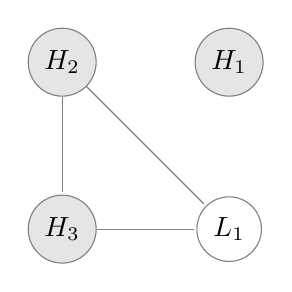
\begin{tikzpicture}[shorten >=1pt,draw=black!50]
	\node (H1) at ( 1.06,  1.06)	[circle, draw, fill = gray!20]	{$H_{1}$};
	\node (H2) at (-1.06,  1.06)	[circle, draw, fill = gray!20]	{$H_{2}$};
	\node (H3) at (-1.06, -1.06)	[circle, draw, fill = gray!20]	{$H_{3}$};
	\node (L1) at ( 1.06, -1.06)	[circle, draw, fill = white]	{$L_{1}$};
	\draw (H2) -- (H3);
	\draw (H2) -- (L1);
	\draw (H3) -- (L1);
\end{tikzpicture}
\end{center}
\columnbreak

\scaleeq{
Equations: \begin{cases}
	e^{H}_{1} \left(\frac{25 \phi}{4} - 4\right) = \alpha - 3 e^{H}_{2} - 3 e^{H}_{3} - 3 e^{L}_{1} \theta - \gamma\\
	e^{H}_{2} \left(\frac{25 \phi}{2} - 2\right) = \alpha - e^{H}_{1} + 2 e^{H}_{3} + 2 e^{L}_{1} \theta - \gamma\\
	e^{H}_{3} \left(\frac{25 \phi}{2} - 2\right) = \alpha - e^{H}_{1} + 2 e^{H}_{2} + 2 e^{L}_{1} \theta - \gamma\\
	e^{L}_{1} \left(\frac{25 \phi}{2 \theta} - 2 \theta\right) = \alpha - e^{H}_{1} + 2 e^{H}_{2} + 2 e^{H}_{3} - \gamma
\end{cases}
}\end{multicols}


Optimal efforts:

\scaleeq{
\begin{cases}
	e^{H}_{1} &= \frac{4 \left(\alpha - \gamma\right) \left(5 \phi - 2 \theta^{2} - 4\right)}{125 \phi^{2} - 20 \phi \theta^{2} - 120 \phi + 8 \theta^{2} + 16}\\
	e^{H}_{2} &= \frac{2 \left(\alpha - \gamma\right) \left(5 \phi - 4\right)}{125 \phi^{2} - 20 \phi \theta^{2} - 120 \phi + 8 \theta^{2} + 16}\\
	e^{H}_{3} &= \frac{2 \left(\alpha - \gamma\right) \left(5 \phi - 4\right)}{125 \phi^{2} - 20 \phi \theta^{2} - 120 \phi + 8 \theta^{2} + 16}\\
	e^{L}_{1} &= \frac{2 \theta \left(\alpha - \gamma\right) \left(5 \phi - 4\right)}{125 \phi^{2} - 20 \phi \theta^{2} - 120 \phi + 8 \theta^{2} + 16}
\end{cases}
}

Production Costs:

\scaleeq{
\begin{cases}
	c^{H}_{1} &= - \frac{20 \alpha \phi - 8 \alpha \theta^{2} - 16 \alpha - 125 \gamma \phi^{2} + 20 \gamma \phi \theta^{2} + 100 \gamma \phi}{125 \phi^{2} - 20 \phi \theta^{2} - 120 \phi + 8 \theta^{2} + 16}\\
	c^{H}_{2} &= - \frac{10 \alpha \phi \theta^{2} + 20 \alpha \phi - 8 \alpha \theta^{2} - 16 \alpha - 125 \gamma \phi^{2} + 10 \gamma \phi \theta^{2} + 100 \gamma \phi}{125 \phi^{2} - 20 \phi \theta^{2} - 120 \phi + 8 \theta^{2} + 16}\\
	c^{H}_{3} &= - \frac{10 \alpha \phi \theta^{2} + 20 \alpha \phi - 8 \alpha \theta^{2} - 16 \alpha - 125 \gamma \phi^{2} + 10 \gamma \phi \theta^{2} + 100 \gamma \phi}{125 \phi^{2} - 20 \phi \theta^{2} - 120 \phi + 8 \theta^{2} + 16}\\
	c^{L}_{1} &= - \frac{10 \alpha \phi \theta^{2} + 20 \alpha \phi - 8 \alpha \theta^{2} - 16 \alpha - 125 \gamma \phi^{2} + 10 \gamma \phi \theta^{2} + 100 \gamma \phi}{125 \phi^{2} - 20 \phi \theta^{2} - 120 \phi + 8 \theta^{2} + 16}
\end{cases}
}

Production Quantities:

\scaleeq{
\begin{cases}
	q^{H}_{1} &= \frac{5 \phi \left(\alpha - \gamma\right) \left(5 \phi - 2 \theta^{2} - 4\right)}{125 \phi^{2} - 20 \phi \theta^{2} - 120 \phi + 8 \theta^{2} + 16}\\
	q^{H}_{2} &= \frac{5 \phi \left(\alpha - \gamma\right) \left(5 \phi - 4\right)}{125 \phi^{2} - 20 \phi \theta^{2} - 120 \phi + 8 \theta^{2} + 16}\\
	q^{H}_{3} &= \frac{5 \phi \left(\alpha - \gamma\right) \left(5 \phi - 4\right)}{125 \phi^{2} - 20 \phi \theta^{2} - 120 \phi + 8 \theta^{2} + 16}\\
	q^{L}_{1} &= \frac{5 \phi \left(\alpha - \gamma\right) \left(5 \phi - 4\right)}{125 \phi^{2} - 20 \phi \theta^{2} - 120 \phi + 8 \theta^{2} + 16}
\end{cases}
}

Profits:

\begin{equation}
\label{eq:E3D:3H1L_profit}
\scaledequation{\begin{cases}
	\pi^{H}_{1} &= \frac{\phi \left(\alpha - \gamma\right)^{2} \left(25 \phi - 16\right) \left(5 \phi - 2 \theta^{2} - 4\right)^{2}}{\left(125 \phi^{2} - 20 \phi \theta^{2} - 120 \phi + 8 \theta^{2} + 16\right)^{2}}\\
	\pi^{H}_{2} &= \frac{\phi \left(\alpha - \gamma\right)^{2} \left(5 \phi - 4\right)^{2} \left(25 \phi - 4\right)}{\left(125 \phi^{2} - 20 \phi \theta^{2} - 120 \phi + 8 \theta^{2} + 16\right)^{2}}\\
	\pi^{H}_{3} &= \frac{\phi \left(\alpha - \gamma\right)^{2} \left(5 \phi - 4\right)^{2} \left(25 \phi - 4\right)}{\left(125 \phi^{2} - 20 \phi \theta^{2} - 120 \phi + 8 \theta^{2} + 16\right)^{2}}\\
	\pi^{L}_{1} &= \frac{\phi \left(\alpha - \gamma\right)^{2} \left(5 \phi - 4\right)^{2} \left(25 \phi - 4 \theta^{2}\right)}{\left(125 \phi^{2} - 20 \phi \theta^{2} - 120 \phi + 8 \theta^{2} + 16\right)^{2}}
\end{cases}
}
\end{equation}

Total Production:

\scaleeq{
\frac{10 \phi \left(\alpha - \gamma\right) \left(10 \phi - \theta^{2} - 8\right)}{125 \phi^{2} - 20 \phi \theta^{2} - 120 \phi + 8 \theta^{2} + 16}
}

Price:

\scaleeq{
\frac{25 \alpha \phi^{2} - 10 \alpha \phi \theta^{2} - 40 \alpha \phi + 8 \alpha \theta^{2} + 16 \alpha + 100 \gamma \phi^{2} - 10 \gamma \phi \theta^{2} - 80 \gamma \phi}{125 \phi^{2} - 20 \phi \theta^{2} - 120 \phi + 8 \theta^{2} + 16}
}

Firm Surplus:

\scaleeq{
\frac{4 \phi \left(\alpha - \gamma\right)^{2} \left(625 \phi^{3} - 150 \phi^{2} \theta^{2} - 1150 \phi^{2} + 25 \phi \theta^{4} + 220 \phi \theta^{2} + 640 \phi - 16 \theta^{4} - 80 \theta^{2} - 96\right)}{\left(125 \phi^{2} - 20 \phi \theta^{2} - 120 \phi + 8 \theta^{2} + 16\right)^{2}}
}

Consumer Surplus:

\scaleeq{
\frac{50 \phi^{2} \left(\alpha - \gamma\right)^{2} \left(10 \phi - \theta^{2} - 8\right)^{2}}{\left(125 \phi^{2} - 20 \phi \theta^{2} - 120 \phi + 8 \theta^{2} + 16\right)^{2}}
}

Social Welfare:

\scaleeq{
\frac{2 \phi \left(\alpha - \gamma\right)^{2} \left(3750 \phi^{3} - 800 \phi^{2} \theta^{2} - 6300 \phi^{2} + 75 \phi \theta^{4} + 840 \phi \theta^{2} + 2880 \phi - 32 \theta^{4} - 160 \theta^{2} - 192\right)}{\left(125 \phi^{2} - 20 \phi \theta^{2} - 120 \phi + 8 \theta^{2} + 16\right)^{2}}
}

%======================================================================

\subsubsection{E3E [3H1L]}
\label{apx:E3E:3H1L}

\begin{multicols}{2}
\begin{center}
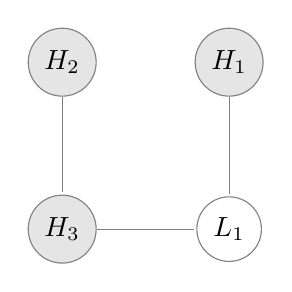
\begin{tikzpicture}[shorten >=1pt,draw=black!50]
	\node (H1) at ( 1.06,  1.06)	[circle, draw, fill = gray!20]	{$H_{1}$};
	\node (H2) at (-1.06,  1.06)	[circle, draw, fill = gray!20]	{$H_{2}$};
	\node (H3) at (-1.06, -1.06)	[circle, draw, fill = gray!20]	{$H_{3}$};
	\node (L1) at ( 1.06, -1.06)	[circle, draw, fill = white]	{$L_{1}$};
	\draw (H1) -- (L1);
	\draw (H2) -- (H3);
	\draw (H3) -- (L1);
\end{tikzpicture}
\end{center}
\columnbreak

\scaleeq{
Equations: \begin{cases}
	e^{H}_{1} \left(\frac{25 \phi}{3} - 3\right) = \alpha - 2 e^{H}_{2} - 3 e^{H}_{3} + 2 e^{L}_{1} \theta - \gamma\\
	e^{H}_{2} \left(\frac{25 \phi}{3} - 3\right) = \alpha - 2 e^{H}_{1} + 2 e^{H}_{3} - 3 e^{L}_{1} \theta - \gamma\\
	e^{H}_{3} \left(\frac{25 \phi}{2} - 2\right) = \alpha - 2 e^{H}_{1} + 3 e^{H}_{2} + 2 e^{L}_{1} \theta - \gamma\\
	e^{L}_{1} \left(\frac{25 \phi}{2 \theta} - 2 \theta\right) = \alpha + 3 e^{H}_{1} - 2 e^{H}_{2} + 2 e^{H}_{3} - \gamma
\end{cases}
}\end{multicols}


Optimal efforts:

\scaleeq{
\begin{cases}
	e^{H}_{1} &= \frac{3 \left(\alpha - \gamma\right) \left(125 \phi^{3} - 125 \phi^{2} + 12 \theta^{2}\right)}{3125 \phi^{4} - 500 \phi^{3} \theta^{2} - 2750 \phi^{3} + 225 \phi^{2} + 240 \phi \theta^{2} - 36 \theta^{2}}\\
	e^{H}_{2} &= \frac{3 \left(\alpha - \gamma\right) \left(125 \phi^{3} - 50 \phi^{2} \theta^{2} - 75 \phi^{2} + 12 \theta^{2}\right)}{3125 \phi^{4} - 500 \phi^{3} \theta^{2} - 2750 \phi^{3} + 225 \phi^{2} + 240 \phi \theta^{2} - 36 \theta^{2}}\\
	e^{H}_{3} &= \frac{10 \phi \left(\alpha - \gamma\right) \left(25 \phi^{2} - 15 \phi - 6 \theta^{2}\right)}{3125 \phi^{4} - 500 \phi^{3} \theta^{2} - 2750 \phi^{3} + 225 \phi^{2} + 240 \phi \theta^{2} - 36 \theta^{2}}\\
	e^{L}_{1} &= \frac{10 \phi \theta \left(\alpha - \gamma\right) \left(25 \phi^{2} - 15 \phi - 6\right)}{3125 \phi^{4} - 500 \phi^{3} \theta^{2} - 2750 \phi^{3} + 225 \phi^{2} + 240 \phi \theta^{2} - 36 \theta^{2}}
\end{cases}
}

Production Costs:

\scaleeq{
\begin{cases}
	c^{H}_{1} &= - \frac{250 \alpha \phi^{3} \theta^{2} + 375 \alpha \phi^{3} - 150 \alpha \phi^{2} \theta^{2} - 375 \alpha \phi^{2} - 60 \alpha \phi \theta^{2} + 36 \alpha \theta^{2} - 3125 \gamma \phi^{4} + 250 \gamma \phi^{3} \theta^{2} + 2375 \gamma \phi^{3} + 150 \gamma \phi^{2} \theta^{2} + 150 \gamma \phi^{2} - 180 \gamma \phi \theta^{2}}{3125 \phi^{4} - 500 \phi^{3} \theta^{2} - 2750 \phi^{3} + 225 \phi^{2} + 240 \phi \theta^{2} - 36 \theta^{2}}\\
	c^{H}_{2} &= - \frac{625 \alpha \phi^{3} - 150 \alpha \phi^{2} \theta^{2} - 375 \alpha \phi^{2} - 60 \alpha \phi \theta^{2} + 36 \alpha \theta^{2} - 3125 \gamma \phi^{4} + 500 \gamma \phi^{3} \theta^{2} + 2125 \gamma \phi^{3} + 150 \gamma \phi^{2} \theta^{2} + 150 \gamma \phi^{2} - 180 \gamma \phi \theta^{2}}{3125 \phi^{4} - 500 \phi^{3} \theta^{2} - 2750 \phi^{3} + 225 \phi^{2} + 240 \phi \theta^{2} - 36 \theta^{2}}\\
	c^{H}_{3} &= - \frac{250 \alpha \phi^{3} \theta^{2} + 625 \alpha \phi^{3} - 300 \alpha \phi^{2} \theta^{2} - 375 \alpha \phi^{2} - 120 \alpha \phi \theta^{2} + 36 \alpha \theta^{2} - 3125 \gamma \phi^{4} + 250 \gamma \phi^{3} \theta^{2} + 2125 \gamma \phi^{3} + 300 \gamma \phi^{2} \theta^{2} + 150 \gamma \phi^{2} - 120 \gamma \phi \theta^{2}}{3125 \phi^{4} - 500 \phi^{3} \theta^{2} - 2750 \phi^{3} + 225 \phi^{2} + 240 \phi \theta^{2} - 36 \theta^{2}}\\
	c^{L}_{1} &= - \frac{250 \alpha \phi^{3} \theta^{2} + 625 \alpha \phi^{3} - 150 \alpha \phi^{2} \theta^{2} - 525 \alpha \phi^{2} - 120 \alpha \phi \theta^{2} + 36 \alpha \theta^{2} - 3125 \gamma \phi^{4} + 250 \gamma \phi^{3} \theta^{2} + 2125 \gamma \phi^{3} + 150 \gamma \phi^{2} \theta^{2} + 300 \gamma \phi^{2} - 120 \gamma \phi \theta^{2}}{3125 \phi^{4} - 500 \phi^{3} \theta^{2} - 2750 \phi^{3} + 225 \phi^{2} + 240 \phi \theta^{2} - 36 \theta^{2}}
\end{cases}
}

Production Quantities:

\scaleeq{
\begin{cases}
	q^{H}_{1} &= \frac{5 \phi \left(\alpha - \gamma\right) \left(125 \phi^{3} - 125 \phi^{2} + 12 \theta^{2}\right)}{3125 \phi^{4} - 500 \phi^{3} \theta^{2} - 2750 \phi^{3} + 225 \phi^{2} + 240 \phi \theta^{2} - 36 \theta^{2}}\\
	q^{H}_{2} &= \frac{5 \phi \left(\alpha - \gamma\right) \left(125 \phi^{3} - 50 \phi^{2} \theta^{2} - 75 \phi^{2} + 12 \theta^{2}\right)}{3125 \phi^{4} - 500 \phi^{3} \theta^{2} - 2750 \phi^{3} + 225 \phi^{2} + 240 \phi \theta^{2} - 36 \theta^{2}}\\
	q^{H}_{3} &= \frac{25 \phi^{2} \left(\alpha - \gamma\right) \left(25 \phi^{2} - 15 \phi - 6 \theta^{2}\right)}{3125 \phi^{4} - 500 \phi^{3} \theta^{2} - 2750 \phi^{3} + 225 \phi^{2} + 240 \phi \theta^{2} - 36 \theta^{2}}\\
	q^{L}_{1} &= \frac{25 \phi^{2} \left(\alpha - \gamma\right) \left(25 \phi^{2} - 15 \phi - 6\right)}{3125 \phi^{4} - 500 \phi^{3} \theta^{2} - 2750 \phi^{3} + 225 \phi^{2} + 240 \phi \theta^{2} - 36 \theta^{2}}
\end{cases}
}

Profits:

\begin{equation}
\label{eq:E3E:3H1L_profit}
\scaledequation{\begin{cases}
	\pi^{H}_{1} &= \frac{\phi \left(\alpha - \gamma\right)^{2} \left(25 \phi - 9\right) \left(125 \phi^{3} - 125 \phi^{2} + 12 \theta^{2}\right)^{2}}{\left(3125 \phi^{4} - 500 \phi^{3} \theta^{2} - 2750 \phi^{3} + 225 \phi^{2} + 240 \phi \theta^{2} - 36 \theta^{2}\right)^{2}}\\
	\pi^{H}_{2} &= \frac{\phi \left(\alpha - \gamma\right)^{2} \left(25 \phi - 9\right) \left(125 \phi^{3} - 50 \phi^{2} \theta^{2} - 75 \phi^{2} + 12 \theta^{2}\right)^{2}}{\left(3125 \phi^{4} - 500 \phi^{3} \theta^{2} - 2750 \phi^{3} + 225 \phi^{2} + 240 \phi \theta^{2} - 36 \theta^{2}\right)^{2}}\\
	\pi^{H}_{3} &= \frac{25 \phi^{3} \left(\alpha - \gamma\right)^{2} \left(25 \phi - 4\right) \left(25 \phi^{2} - 15 \phi - 6 \theta^{2}\right)^{2}}{\left(3125 \phi^{4} - 500 \phi^{3} \theta^{2} - 2750 \phi^{3} + 225 \phi^{2} + 240 \phi \theta^{2} - 36 \theta^{2}\right)^{2}}\\
	\pi^{L}_{1} &= \frac{25 \phi^{3} \left(\alpha - \gamma\right)^{2} \left(25 \phi - 4 \theta^{2}\right) \left(25 \phi^{2} - 15 \phi - 6\right)^{2}}{\left(3125 \phi^{4} - 500 \phi^{3} \theta^{2} - 2750 \phi^{3} + 225 \phi^{2} + 240 \phi \theta^{2} - 36 \theta^{2}\right)^{2}}
\end{cases}
}
\end{equation}

Total Production:

\scaleeq{
\frac{10 \phi \left(\alpha - \gamma\right) \left(250 \phi^{3} - 25 \phi^{2} \theta^{2} - 175 \phi^{2} - 15 \phi \theta^{2} - 15 \phi + 12 \theta^{2}\right)}{3125 \phi^{4} - 500 \phi^{3} \theta^{2} - 2750 \phi^{3} + 225 \phi^{2} + 240 \phi \theta^{2} - 36 \theta^{2}}
}

Price:

\scaleeq{
\frac{625 \alpha \phi^{4} - 250 \alpha \phi^{3} \theta^{2} - 1000 \alpha \phi^{3} + 150 \alpha \phi^{2} \theta^{2} + 375 \alpha \phi^{2} + 120 \alpha \phi \theta^{2} - 36 \alpha \theta^{2} + 2500 \gamma \phi^{4} - 250 \gamma \phi^{3} \theta^{2} - 1750 \gamma \phi^{3} - 150 \gamma \phi^{2} \theta^{2} - 150 \gamma \phi^{2} + 120 \gamma \phi \theta^{2}}{3125 \phi^{4} - 500 \phi^{3} \theta^{2} - 2750 \phi^{3} + 225 \phi^{2} + 240 \phi \theta^{2} - 36 \theta^{2}}
}

Firm Surplus:

\scaleeq{
\frac{2 \phi \left(\alpha - \gamma\right)^{2} \left(781250 \phi^{7} - 187500 \phi^{6} \theta^{2} - 1265625 \phi^{6} + 31250 \phi^{5} \theta^{4} + 93750 \phi^{5} \theta^{2} + 575000 \phi^{5} - 11250 \phi^{4} \theta^{4} + 116250 \phi^{4} \theta^{2} - 50625 \phi^{4} - 3750 \phi^{3} \theta^{4} - 105000 \phi^{3} \theta^{2} + 11250 \phi^{3} + 3600 \phi^{2} \theta^{4} + 19800 \phi^{2} \theta^{2} + 3600 \phi \theta^{4} - 1296 \theta^{4}\right)}{\left(3125 \phi^{4} - 500 \phi^{3} \theta^{2} - 2750 \phi^{3} + 225 \phi^{2} + 240 \phi \theta^{2} - 36 \theta^{2}\right)^{2}}
}

Consumer Surplus:

\scaleeq{
\frac{50 \phi^{2} \left(\alpha - \gamma\right)^{2} \left(250 \phi^{3} - 25 \phi^{2} \theta^{2} - 175 \phi^{2} - 15 \phi \theta^{2} - 15 \phi + 12 \theta^{2}\right)^{2}}{\left(3125 \phi^{4} - 500 \phi^{3} \theta^{2} - 2750 \phi^{3} + 225 \phi^{2} + 240 \phi \theta^{2} - 36 \theta^{2}\right)^{2}}
}

Social Welfare:

\scaleeq{
\frac{2 \phi \left(\alpha - \gamma\right)^{2} \left(2343750 \phi^{7} - 500000 \phi^{6} \theta^{2} - 3453125 \phi^{6} + 46875 \phi^{5} \theta^{4} + 125000 \phi^{5} \theta^{2} + 1153125 \phi^{5} + 7500 \phi^{4} \theta^{4} + 416250 \phi^{4} \theta^{2} + 80625 \phi^{4} - 13125 \phi^{3} \theta^{4} - 198750 \phi^{3} \theta^{2} + 16875 \phi^{3} - 5400 \phi^{2} \theta^{4} + 10800 \phi^{2} \theta^{2} + 7200 \phi \theta^{4} - 1296 \theta^{4}\right)}{\left(3125 \phi^{4} - 500 \phi^{3} \theta^{2} - 2750 \phi^{3} + 225 \phi^{2} + 240 \phi \theta^{2} - 36 \theta^{2}\right)^{2}}
}

%======================================================================

\subsubsection{E3F [3H1L]}
\label{apx:E3F:3H1L}

\begin{multicols}{2}
\begin{center}
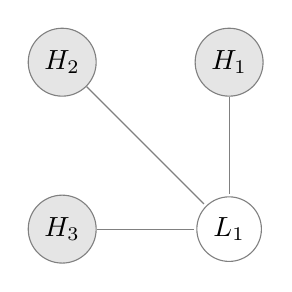
\begin{tikzpicture}[shorten >=1pt,draw=black!50]
	\node (H1) at ( 1.06,  1.06)	[circle, draw, fill = gray!20]	{$H_{1}$};
	\node (H2) at (-1.06,  1.06)	[circle, draw, fill = gray!20]	{$H_{2}$};
	\node (H3) at (-1.06, -1.06)	[circle, draw, fill = gray!20]	{$H_{3}$};
	\node (L1) at ( 1.06, -1.06)	[circle, draw, fill = white]	{$L_{1}$};
	\draw (H1) -- (L1);
	\draw (H2) -- (L1);
	\draw (H3) -- (L1);
\end{tikzpicture}
\end{center}
\columnbreak

\scaleeq{
Equations: \begin{cases}
	e^{H}_{1} \left(\frac{25 \phi}{3} - 3\right) = \alpha - 2 e^{H}_{2} - 2 e^{H}_{3} + e^{L}_{1} \theta - \gamma\\
	e^{H}_{2} \left(\frac{25 \phi}{3} - 3\right) = \alpha - 2 e^{H}_{1} - 2 e^{H}_{3} + e^{L}_{1} \theta - \gamma\\
	e^{H}_{3} \left(\frac{25 \phi}{3} - 3\right) = \alpha - 2 e^{H}_{1} - 2 e^{H}_{2} + e^{L}_{1} \theta - \gamma\\
	e^{L}_{1} \left(\frac{25 \phi}{\theta} - \theta\right) = \alpha + 3 e^{H}_{1} + 3 e^{H}_{2} + 3 e^{H}_{3} - \gamma
\end{cases}
}\end{multicols}


Optimal efforts:

\scaleeq{
\begin{cases}
	e^{H}_{1} &= \frac{15 \phi \left(\alpha - \gamma\right)}{125 \phi^{2} - 5 \phi \theta^{2} + 15 \phi - 6 \theta^{2}}\\
	e^{H}_{2} &= \frac{15 \phi \left(\alpha - \gamma\right)}{125 \phi^{2} - 5 \phi \theta^{2} + 15 \phi - 6 \theta^{2}}\\
	e^{H}_{3} &= \frac{15 \phi \left(\alpha - \gamma\right)}{125 \phi^{2} - 5 \phi \theta^{2} + 15 \phi - 6 \theta^{2}}\\
	e^{L}_{1} &= \frac{\theta \left(\alpha - \gamma\right) \left(5 \phi + 6\right)}{125 \phi^{2} - 5 \phi \theta^{2} + 15 \phi - 6 \theta^{2}}
\end{cases}
}

Production Costs:

\scaleeq{
\begin{cases}
	c^{H}_{1} &= - \frac{5 \alpha \phi \theta^{2} + 15 \alpha \phi + 6 \alpha \theta^{2} - 125 \gamma \phi^{2} - 30 \gamma \phi}{125 \phi^{2} - 5 \phi \theta^{2} + 15 \phi - 6 \theta^{2}}\\
	c^{H}_{2} &= - \frac{5 \alpha \phi \theta^{2} + 15 \alpha \phi + 6 \alpha \theta^{2} - 125 \gamma \phi^{2} - 30 \gamma \phi}{125 \phi^{2} - 5 \phi \theta^{2} + 15 \phi - 6 \theta^{2}}\\
	c^{H}_{3} &= - \frac{5 \alpha \phi \theta^{2} + 15 \alpha \phi + 6 \alpha \theta^{2} - 125 \gamma \phi^{2} - 30 \gamma \phi}{125 \phi^{2} - 5 \phi \theta^{2} + 15 \phi - 6 \theta^{2}}\\
	c^{L}_{1} &= - \frac{5 \alpha \phi \theta^{2} + 45 \alpha \phi + 6 \alpha \theta^{2} - 125 \gamma \phi^{2} - 60 \gamma \phi}{125 \phi^{2} - 5 \phi \theta^{2} + 15 \phi - 6 \theta^{2}}
\end{cases}
}

Production Quantities:

\scaleeq{
\begin{cases}
	q^{H}_{1} &= \frac{25 \phi^{2} \left(\alpha - \gamma\right)}{125 \phi^{2} - 5 \phi \theta^{2} + 15 \phi - 6 \theta^{2}}\\
	q^{H}_{2} &= \frac{25 \phi^{2} \left(\alpha - \gamma\right)}{125 \phi^{2} - 5 \phi \theta^{2} + 15 \phi - 6 \theta^{2}}\\
	q^{H}_{3} &= \frac{25 \phi^{2} \left(\alpha - \gamma\right)}{125 \phi^{2} - 5 \phi \theta^{2} + 15 \phi - 6 \theta^{2}}\\
	q^{L}_{1} &= \frac{5 \phi \left(\alpha - \gamma\right) \left(5 \phi + 6\right)}{125 \phi^{2} - 5 \phi \theta^{2} + 15 \phi - 6 \theta^{2}}
\end{cases}
}

Profits:

\begin{equation}
\label{eq:E3F:3H1L_profit}
\scaledequation{\begin{cases}
	\pi^{H}_{1} &= \frac{25 \phi^{3} \left(\alpha - \gamma\right)^{2} \left(25 \phi - 9\right)}{\left(125 \phi^{2} - 5 \phi \theta^{2} + 15 \phi - 6 \theta^{2}\right)^{2}}\\
	\pi^{H}_{2} &= \frac{25 \phi^{3} \left(\alpha - \gamma\right)^{2} \left(25 \phi - 9\right)}{\left(125 \phi^{2} - 5 \phi \theta^{2} + 15 \phi - 6 \theta^{2}\right)^{2}}\\
	\pi^{H}_{3} &= \frac{25 \phi^{3} \left(\alpha - \gamma\right)^{2} \left(25 \phi - 9\right)}{\left(125 \phi^{2} - 5 \phi \theta^{2} + 15 \phi - 6 \theta^{2}\right)^{2}}\\
	\pi^{L}_{1} &= \frac{\phi \left(\alpha - \gamma\right)^{2} \left(5 \phi + 6\right)^{2} \left(25 \phi - \theta^{2}\right)}{\left(125 \phi^{2} - 5 \phi \theta^{2} + 15 \phi - 6 \theta^{2}\right)^{2}}
\end{cases}
}
\end{equation}

Total Production:

\scaleeq{
\frac{10 \phi \left(\alpha - \gamma\right) \left(10 \phi + 3\right)}{125 \phi^{2} - 5 \phi \theta^{2} + 15 \phi - 6 \theta^{2}}
}

Price:

\scaleeq{
\frac{25 \alpha \phi^{2} - 5 \alpha \phi \theta^{2} - 15 \alpha \phi - 6 \alpha \theta^{2} + 100 \gamma \phi^{2} + 30 \gamma \phi}{125 \phi^{2} - 5 \phi \theta^{2} + 15 \phi - 6 \theta^{2}}
}

Firm Surplus:

\scaleeq{
\frac{\phi \left(\alpha - \gamma\right)^{2} \left(2500 \phi^{3} - 25 \phi^{2} \theta^{2} + 825 \phi^{2} - 60 \phi \theta^{2} + 900 \phi - 36 \theta^{2}\right)}{\left(125 \phi^{2} - 5 \phi \theta^{2} + 15 \phi - 6 \theta^{2}\right)^{2}}
}

Consumer Surplus:

\scaleeq{
\frac{50 \phi^{2} \left(\alpha - \gamma\right)^{2} \left(10 \phi + 3\right)^{2}}{\left(125 \phi^{2} - 5 \phi \theta^{2} + 15 \phi - 6 \theta^{2}\right)^{2}}
}

Social Welfare:

\scaleeq{
\frac{\phi \left(\alpha - \gamma\right)^{2} \left(7500 \phi^{3} - 25 \phi^{2} \theta^{2} + 3825 \phi^{2} - 60 \phi \theta^{2} + 1350 \phi - 36 \theta^{2}\right)}{\left(125 \phi^{2} - 5 \phi \theta^{2} + 15 \phi - 6 \theta^{2}\right)^{2}}
}

%======================================================================

\subsubsection{E4A [3H1L]}
\label{apx:E4A:3H1L}

\begin{multicols}{2}
\begin{center}
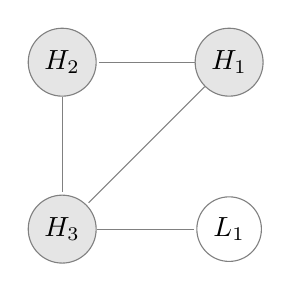
\begin{tikzpicture}[shorten >=1pt,draw=black!50]
	\node (H1) at ( 1.06,  1.06)	[circle, draw, fill = gray!20]	{$H_{1}$};
	\node (H2) at (-1.06,  1.06)	[circle, draw, fill = gray!20]	{$H_{2}$};
	\node (H3) at (-1.06, -1.06)	[circle, draw, fill = gray!20]	{$H_{3}$};
	\node (L1) at ( 1.06, -1.06)	[circle, draw, fill = white]	{$L_{1}$};
	\draw (H1) -- (H2);
	\draw (H1) -- (H3);
	\draw (H2) -- (H3);
	\draw (H3) -- (L1);
\end{tikzpicture}
\end{center}
\columnbreak

\scaleeq{
Equations: \begin{cases}
	e^{H}_{1} \left(\frac{25 \phi}{2} - 2\right) = \alpha + 2 e^{H}_{2} + e^{H}_{3} - 2 e^{L}_{1} \theta - \gamma\\
	e^{H}_{2} \left(\frac{25 \phi}{2} - 2\right) = \alpha + 2 e^{H}_{1} + e^{H}_{3} - 2 e^{L}_{1} \theta - \gamma\\
	e^{H}_{3} \left(25 \phi - 1\right) = \alpha + 2 e^{H}_{1} + 2 e^{H}_{2} + 3 e^{L}_{1} \theta - \gamma\\
	e^{L}_{1} \left(\frac{25 \phi}{3 \theta} - 3 \theta\right) = \alpha - 3 e^{H}_{1} - 3 e^{H}_{2} + e^{H}_{3} - \gamma
\end{cases}
}\end{multicols}


Optimal efforts:

\scaleeq{
\begin{cases}
	e^{H}_{1} &= \frac{10 \phi \left(\alpha - \gamma\right) \left(5 \phi - 3 \theta^{2}\right)}{625 \phi^{3} - 225 \phi^{2} \theta^{2} - 225 \phi^{2} + 12 \theta^{2}}\\
	e^{H}_{2} &= \frac{10 \phi \left(\alpha - \gamma\right) \left(5 \phi - 3 \theta^{2}\right)}{625 \phi^{3} - 225 \phi^{2} \theta^{2} - 225 \phi^{2} + 12 \theta^{2}}\\
	e^{H}_{3} &= \frac{\left(\alpha - \gamma\right) \left(25 \phi^{2} - 12 \theta^{2}\right)}{625 \phi^{3} - 225 \phi^{2} \theta^{2} - 225 \phi^{2} + 12 \theta^{2}}\\
	e^{L}_{1} &= \frac{15 \phi \theta \left(\alpha - \gamma\right) \left(5 \phi - 4\right)}{625 \phi^{3} - 225 \phi^{2} \theta^{2} - 225 \phi^{2} + 12 \theta^{2}}
\end{cases}
}

Production Costs:

\scaleeq{
\begin{cases}
	c^{H}_{1} &= - \frac{125 \alpha \phi^{2} - 60 \alpha \phi \theta^{2} - 12 \alpha \theta^{2} - 625 \gamma \phi^{3} + 225 \gamma \phi^{2} \theta^{2} + 100 \gamma \phi^{2} + 60 \gamma \phi \theta^{2}}{625 \phi^{3} - 225 \phi^{2} \theta^{2} - 225 \phi^{2} + 12 \theta^{2}}\\
	c^{H}_{2} &= - \frac{125 \alpha \phi^{2} - 60 \alpha \phi \theta^{2} - 12 \alpha \theta^{2} - 625 \gamma \phi^{3} + 225 \gamma \phi^{2} \theta^{2} + 100 \gamma \phi^{2} + 60 \gamma \phi \theta^{2}}{625 \phi^{3} - 225 \phi^{2} \theta^{2} - 225 \phi^{2} + 12 \theta^{2}}\\
	c^{H}_{3} &= - \frac{75 \alpha \phi^{2} \theta^{2} + 125 \alpha \phi^{2} - 120 \alpha \phi \theta^{2} - 12 \alpha \theta^{2} - 625 \gamma \phi^{3} + 150 \gamma \phi^{2} \theta^{2} + 100 \gamma \phi^{2} + 120 \gamma \phi \theta^{2}}{625 \phi^{3} - 225 \phi^{2} \theta^{2} - 225 \phi^{2} + 12 \theta^{2}}\\
	c^{L}_{1} &= - \frac{75 \alpha \phi^{2} \theta^{2} + 25 \alpha \phi^{2} - 60 \alpha \phi \theta^{2} - 12 \alpha \theta^{2} - 625 \gamma \phi^{3} + 150 \gamma \phi^{2} \theta^{2} + 200 \gamma \phi^{2} + 60 \gamma \phi \theta^{2}}{625 \phi^{3} - 225 \phi^{2} \theta^{2} - 225 \phi^{2} + 12 \theta^{2}}
\end{cases}
}

Production Quantities:

\scaleeq{
\begin{cases}
	q^{H}_{1} &= \frac{25 \phi^{2} \left(\alpha - \gamma\right) \left(5 \phi - 3 \theta^{2}\right)}{625 \phi^{3} - 225 \phi^{2} \theta^{2} - 225 \phi^{2} + 12 \theta^{2}}\\
	q^{H}_{2} &= \frac{25 \phi^{2} \left(\alpha - \gamma\right) \left(5 \phi - 3 \theta^{2}\right)}{625 \phi^{3} - 225 \phi^{2} \theta^{2} - 225 \phi^{2} + 12 \theta^{2}}\\
	q^{H}_{3} &= \frac{5 \phi \left(\alpha - \gamma\right) \left(25 \phi^{2} - 12 \theta^{2}\right)}{625 \phi^{3} - 225 \phi^{2} \theta^{2} - 225 \phi^{2} + 12 \theta^{2}}\\
	q^{L}_{1} &= \frac{25 \phi^{2} \left(\alpha - \gamma\right) \left(5 \phi - 4\right)}{625 \phi^{3} - 225 \phi^{2} \theta^{2} - 225 \phi^{2} + 12 \theta^{2}}
\end{cases}
}

Profits:

\begin{equation}
\label{eq:E4A:3H1L_profit}
\scaledequation{\begin{cases}
	\pi^{H}_{1} &= \frac{25 \phi^{3} \left(\alpha - \gamma\right)^{2} \left(5 \phi - 3 \theta^{2}\right)^{2} \left(25 \phi - 4\right)}{\left(625 \phi^{3} - 225 \phi^{2} \theta^{2} - 225 \phi^{2} + 12 \theta^{2}\right)^{2}}\\
	\pi^{H}_{2} &= \frac{25 \phi^{3} \left(\alpha - \gamma\right)^{2} \left(5 \phi - 3 \theta^{2}\right)^{2} \left(25 \phi - 4\right)}{\left(625 \phi^{3} - 225 \phi^{2} \theta^{2} - 225 \phi^{2} + 12 \theta^{2}\right)^{2}}\\
	\pi^{H}_{3} &= \frac{\phi \left(\alpha - \gamma\right)^{2} \left(25 \phi - 1\right) \left(25 \phi^{2} - 12 \theta^{2}\right)^{2}}{\left(625 \phi^{3} - 225 \phi^{2} \theta^{2} - 225 \phi^{2} + 12 \theta^{2}\right)^{2}}\\
	\pi^{L}_{1} &= \frac{25 \phi^{3} \left(\alpha - \gamma\right)^{2} \left(5 \phi - 4\right)^{2} \left(25 \phi - 9 \theta^{2}\right)}{\left(625 \phi^{3} - 225 \phi^{2} \theta^{2} - 225 \phi^{2} + 12 \theta^{2}\right)^{2}}
\end{cases}
}
\end{equation}

Total Production:

\scaleeq{
\frac{10 \phi \left(\alpha - \gamma\right) \left(50 \phi^{2} - 15 \phi \theta^{2} - 10 \phi - 6 \theta^{2}\right)}{625 \phi^{3} - 225 \phi^{2} \theta^{2} - 225 \phi^{2} + 12 \theta^{2}}
}

Price:

\scaleeq{
\frac{125 \alpha \phi^{3} - 75 \alpha \phi^{2} \theta^{2} - 125 \alpha \phi^{2} + 60 \alpha \phi \theta^{2} + 12 \alpha \theta^{2} + 500 \gamma \phi^{3} - 150 \gamma \phi^{2} \theta^{2} - 100 \gamma \phi^{2} - 60 \gamma \phi \theta^{2}}{625 \phi^{3} - 225 \phi^{2} \theta^{2} - 225 \phi^{2} + 12 \theta^{2}}
}

Firm Surplus:

\scaleeq{
\frac{\phi \left(\alpha - \gamma\right)^{2} \left(62500 \phi^{5} - 43125 \phi^{4} \theta^{2} - 30625 \phi^{4} + 11250 \phi^{3} \theta^{4} + 10000 \phi^{3} - 1800 \phi^{2} \theta^{4} - 3000 \phi^{2} \theta^{2} + 3600 \phi \theta^{4} - 144 \theta^{4}\right)}{\left(625 \phi^{3} - 225 \phi^{2} \theta^{2} - 225 \phi^{2} + 12 \theta^{2}\right)^{2}}
}

Consumer Surplus:

\scaleeq{
\frac{50 \phi^{2} \left(\alpha - \gamma\right)^{2} \left(50 \phi^{2} - 15 \phi \theta^{2} - 10 \phi - 6 \theta^{2}\right)^{2}}{\left(625 \phi^{3} - 225 \phi^{2} \theta^{2} - 225 \phi^{2} + 12 \theta^{2}\right)^{2}}
}

Social Welfare:

\scaleeq{
\frac{3 \phi \left(\alpha - \gamma\right)^{2} \left(62500 \phi^{5} - 39375 \phi^{4} \theta^{2} - 26875 \phi^{4} + 7500 \phi^{3} \theta^{4} - 5000 \phi^{3} \theta^{2} + 5000 \phi^{3} + 2400 \phi^{2} \theta^{4} + 1000 \phi^{2} \theta^{2} + 1800 \phi \theta^{4} - 48 \theta^{4}\right)}{\left(625 \phi^{3} - 225 \phi^{2} \theta^{2} - 225 \phi^{2} + 12 \theta^{2}\right)^{2}}
}

%======================================================================

\subsubsection{E4B [3H1L]}
\label{apx:E4B:3H1L}

\begin{multicols}{2}
\begin{center}
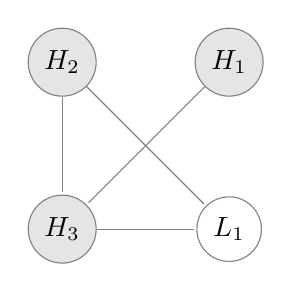
\begin{tikzpicture}[shorten >=1pt,draw=black!50]
	\node (H1) at ( 1.06,  1.06)	[circle, draw, fill = gray!20]	{$H_{1}$};
	\node (H2) at (-1.06,  1.06)	[circle, draw, fill = gray!20]	{$H_{2}$};
	\node (H3) at (-1.06, -1.06)	[circle, draw, fill = gray!20]	{$H_{3}$};
	\node (L1) at ( 1.06, -1.06)	[circle, draw, fill = white]	{$L_{1}$};
	\draw (H1) -- (H3);
	\draw (H2) -- (H3);
	\draw (H2) -- (L1);
	\draw (H3) -- (L1);
\end{tikzpicture}
\end{center}
\columnbreak

\scaleeq{
Equations: \begin{cases}
	e^{H}_{1} \left(\frac{25 \phi}{3} - 3\right) = \alpha - 3 e^{H}_{2} + e^{H}_{3} - 3 e^{L}_{1} \theta - \gamma\\
	e^{H}_{2} \left(\frac{25 \phi}{2} - 2\right) = \alpha - 2 e^{H}_{1} + e^{H}_{3} + 2 e^{L}_{1} \theta - \gamma\\
	e^{H}_{3} \left(25 \phi - 1\right) = \alpha + 3 e^{H}_{1} + 2 e^{H}_{2} + 2 e^{L}_{1} \theta - \gamma\\
	e^{L}_{1} \left(\frac{25 \phi}{2 \theta} - 2 \theta\right) = \alpha - 2 e^{H}_{1} + 2 e^{H}_{2} + e^{H}_{3} - \gamma
\end{cases}
}\end{multicols}


Optimal efforts:

\scaleeq{
\begin{cases}
	e^{H}_{1} &= \frac{15 \phi \left(\alpha - \gamma\right) \left(5 \phi - 2 \theta^{2} - 2\right)}{625 \phi^{3} - 100 \phi^{2} \theta^{2} - 350 \phi^{2} + 6 \theta^{2} + 6}\\
	e^{H}_{2} &= \frac{10 \phi \left(\alpha - \gamma\right) \left(5 \phi - 3\right)}{625 \phi^{3} - 100 \phi^{2} \theta^{2} - 350 \phi^{2} + 6 \theta^{2} + 6}\\
	e^{H}_{3} &= \frac{\left(\alpha - \gamma\right) \left(25 \phi^{2} - 6 \theta^{2} - 6\right)}{625 \phi^{3} - 100 \phi^{2} \theta^{2} - 350 \phi^{2} + 6 \theta^{2} + 6}\\
	e^{L}_{1} &= \frac{10 \phi \theta \left(\alpha - \gamma\right) \left(5 \phi - 3\right)}{625 \phi^{3} - 100 \phi^{2} \theta^{2} - 350 \phi^{2} + 6 \theta^{2} + 6}
\end{cases}
}

Production Costs:

\scaleeq{
\begin{cases}
	c^{H}_{1} &= - \frac{100 \alpha \phi^{2} - 30 \alpha \phi \theta^{2} - 30 \alpha \phi - 6 \alpha \theta^{2} - 6 \alpha - 625 \gamma \phi^{3} + 100 \gamma \phi^{2} \theta^{2} + 250 \gamma \phi^{2} + 30 \gamma \phi \theta^{2} + 30 \gamma \phi}{625 \phi^{3} - 100 \phi^{2} \theta^{2} - 350 \phi^{2} + 6 \theta^{2} + 6}\\
	c^{H}_{2} &= - \frac{50 \alpha \phi^{2} \theta^{2} + 75 \alpha \phi^{2} - 30 \alpha \phi \theta^{2} - 30 \alpha \phi - 6 \alpha \theta^{2} - 6 \alpha - 625 \gamma \phi^{3} + 50 \gamma \phi^{2} \theta^{2} + 275 \gamma \phi^{2} + 30 \gamma \phi \theta^{2} + 30 \gamma \phi}{625 \phi^{3} - 100 \phi^{2} \theta^{2} - 350 \phi^{2} + 6 \theta^{2} + 6}\\
	c^{H}_{3} &= - \frac{50 \alpha \phi^{2} \theta^{2} + 150 \alpha \phi^{2} - 60 \alpha \phi \theta^{2} - 60 \alpha \phi - 6 \alpha \theta^{2} - 6 \alpha - 625 \gamma \phi^{3} + 50 \gamma \phi^{2} \theta^{2} + 200 \gamma \phi^{2} + 60 \gamma \phi \theta^{2} + 60 \gamma \phi}{625 \phi^{3} - 100 \phi^{2} \theta^{2} - 350 \phi^{2} + 6 \theta^{2} + 6}\\
	c^{L}_{1} &= - \frac{50 \alpha \phi^{2} \theta^{2} + 75 \alpha \phi^{2} - 30 \alpha \phi \theta^{2} - 30 \alpha \phi - 6 \alpha \theta^{2} - 6 \alpha - 625 \gamma \phi^{3} + 50 \gamma \phi^{2} \theta^{2} + 275 \gamma \phi^{2} + 30 \gamma \phi \theta^{2} + 30 \gamma \phi}{625 \phi^{3} - 100 \phi^{2} \theta^{2} - 350 \phi^{2} + 6 \theta^{2} + 6}
\end{cases}
}

Production Quantities:

\scaleeq{
\begin{cases}
	q^{H}_{1} &= \frac{25 \phi^{2} \left(\alpha - \gamma\right) \left(5 \phi - 2 \theta^{2} - 2\right)}{625 \phi^{3} - 100 \phi^{2} \theta^{2} - 350 \phi^{2} + 6 \theta^{2} + 6}\\
	q^{H}_{2} &= \frac{25 \phi^{2} \left(\alpha - \gamma\right) \left(5 \phi - 3\right)}{625 \phi^{3} - 100 \phi^{2} \theta^{2} - 350 \phi^{2} + 6 \theta^{2} + 6}\\
	q^{H}_{3} &= \frac{5 \phi \left(\alpha - \gamma\right) \left(25 \phi^{2} - 6 \theta^{2} - 6\right)}{625 \phi^{3} - 100 \phi^{2} \theta^{2} - 350 \phi^{2} + 6 \theta^{2} + 6}\\
	q^{L}_{1} &= \frac{25 \phi^{2} \left(\alpha - \gamma\right) \left(5 \phi - 3\right)}{625 \phi^{3} - 100 \phi^{2} \theta^{2} - 350 \phi^{2} + 6 \theta^{2} + 6}
\end{cases}
}

Profits:

\begin{equation}
\label{eq:E4B:3H1L_profit}
\scaledequation{\begin{cases}
	\pi^{H}_{1} &= \frac{25 \phi^{3} \left(\alpha - \gamma\right)^{2} \left(25 \phi - 9\right) \left(5 \phi - 2 \theta^{2} - 2\right)^{2}}{\left(625 \phi^{3} - 100 \phi^{2} \theta^{2} - 350 \phi^{2} + 6 \theta^{2} + 6\right)^{2}}\\
	\pi^{H}_{2} &= \frac{25 \phi^{3} \left(\alpha - \gamma\right)^{2} \left(5 \phi - 3\right)^{2} \left(25 \phi - 4\right)}{\left(625 \phi^{3} - 100 \phi^{2} \theta^{2} - 350 \phi^{2} + 6 \theta^{2} + 6\right)^{2}}\\
	\pi^{H}_{3} &= \frac{\phi \left(\alpha - \gamma\right)^{2} \left(25 \phi - 1\right) \left(25 \phi^{2} - 6 \theta^{2} - 6\right)^{2}}{\left(625 \phi^{3} - 100 \phi^{2} \theta^{2} - 350 \phi^{2} + 6 \theta^{2} + 6\right)^{2}}\\
	\pi^{L}_{1} &= \frac{25 \phi^{3} \left(\alpha - \gamma\right)^{2} \left(5 \phi - 3\right)^{2} \left(25 \phi - 4 \theta^{2}\right)}{\left(625 \phi^{3} - 100 \phi^{2} \theta^{2} - 350 \phi^{2} + 6 \theta^{2} + 6\right)^{2}}
\end{cases}
}
\end{equation}

Total Production:

\scaleeq{
\frac{10 \phi \left(\alpha - \gamma\right) \left(50 \phi^{2} - 5 \phi \theta^{2} - 20 \phi - 3 \theta^{2} - 3\right)}{625 \phi^{3} - 100 \phi^{2} \theta^{2} - 350 \phi^{2} + 6 \theta^{2} + 6}
}

Price:

\scaleeq{
\frac{125 \alpha \phi^{3} - 50 \alpha \phi^{2} \theta^{2} - 150 \alpha \phi^{2} + 30 \alpha \phi \theta^{2} + 30 \alpha \phi + 6 \alpha \theta^{2} + 6 \alpha + 500 \gamma \phi^{3} - 50 \gamma \phi^{2} \theta^{2} - 200 \gamma \phi^{2} - 30 \gamma \phi \theta^{2} - 30 \gamma \phi}{625 \phi^{3} - 100 \phi^{2} \theta^{2} - 350 \phi^{2} + 6 \theta^{2} + 6}
}

Firm Surplus:

\scaleeq{
\frac{2 \phi \left(\alpha - \gamma\right)^{2} \left(31250 \phi^{5} - 7500 \phi^{4} \theta^{2} - 29375 \phi^{4} + 1250 \phi^{3} \theta^{4} + 2500 \phi^{3} \theta^{2} + 6875 \phi^{3} - 450 \phi^{2} \theta^{4} - 1200 \phi^{2} \theta^{2} - 750 \phi^{2} + 450 \phi \theta^{4} + 900 \phi \theta^{2} + 450 \phi - 18 \theta^{4} - 36 \theta^{2} - 18\right)}{\left(625 \phi^{3} - 100 \phi^{2} \theta^{2} - 350 \phi^{2} + 6 \theta^{2} + 6\right)^{2}}
}

Consumer Surplus:

\scaleeq{
\frac{50 \phi^{2} \left(\alpha - \gamma\right)^{2} \left(50 \phi^{2} - 5 \phi \theta^{2} - 20 \phi - 3 \theta^{2} - 3\right)^{2}}{\left(625 \phi^{3} - 100 \phi^{2} \theta^{2} - 350 \phi^{2} + 6 \theta^{2} + 6\right)^{2}}
}

Social Welfare:

\scaleeq{
\frac{2 \phi \left(\alpha - \gamma\right)^{2} \left(93750 \phi^{5} - 20000 \phi^{4} \theta^{2} - 79375 \phi^{4} + 1875 \phi^{3} \theta^{4} + 9375 \phi^{3} + 300 \phi^{2} \theta^{4} + 2550 \phi^{2} \theta^{2} + 2250 \phi^{2} + 675 \phi \theta^{4} + 1350 \phi \theta^{2} + 675 \phi - 18 \theta^{4} - 36 \theta^{2} - 18\right)}{\left(625 \phi^{3} - 100 \phi^{2} \theta^{2} - 350 \phi^{2} + 6 \theta^{2} + 6\right)^{2}}
}

%======================================================================

\subsubsection{E4C [3H1L]}
\label{apx:E4C:3H1L}

\begin{multicols}{2}
\begin{center}
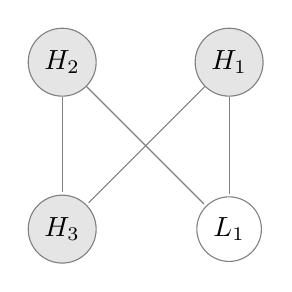
\begin{tikzpicture}[shorten >=1pt,draw=black!50]
	\node (H1) at ( 1.06,  1.06)	[circle, draw, fill = gray!20]	{$H_{1}$};
	\node (H2) at (-1.06,  1.06)	[circle, draw, fill = gray!20]	{$H_{2}$};
	\node (H3) at (-1.06, -1.06)	[circle, draw, fill = gray!20]	{$H_{3}$};
	\node (L1) at ( 1.06, -1.06)	[circle, draw, fill = white]	{$L_{1}$};
	\draw (H1) -- (H3);
	\draw (H1) -- (L1);
	\draw (H2) -- (H3);
	\draw (H2) -- (L1);
\end{tikzpicture}
\end{center}
\columnbreak

\scaleeq{
Equations: \begin{cases}
	e^{H}_{1} \left(\frac{25 \phi}{2} - 2\right) = \alpha - 3 e^{H}_{2} + 2 e^{H}_{3} + 2 e^{L}_{1} \theta - \gamma\\
	e^{H}_{2} \left(\frac{25 \phi}{2} - 2\right) = \alpha - 3 e^{H}_{1} + 2 e^{H}_{3} + 2 e^{L}_{1} \theta - \gamma\\
	e^{H}_{3} \left(\frac{25 \phi}{2} - 2\right) = \alpha + 2 e^{H}_{1} + 2 e^{H}_{2} - 3 e^{L}_{1} \theta - \gamma\\
	e^{L}_{1} \left(\frac{25 \phi}{2 \theta} - 2 \theta\right) = \alpha + 2 e^{H}_{1} + 2 e^{H}_{2} - 3 e^{H}_{3} - \gamma
\end{cases}
}\end{multicols}


Optimal efforts:

\scaleeq{
\begin{cases}
	e^{H}_{1} &= \frac{2 \left(\alpha - \gamma\right) \left(5 \phi - 2 \theta\right) \left(5 \phi + 2 \theta\right)}{625 \phi^{3} - 100 \phi^{2} \theta^{2} - 50 \phi^{2} - 60 \phi \theta^{2} - 40 \phi + 24 \theta^{2}}\\
	e^{H}_{2} &= \frac{2 \left(\alpha - \gamma\right) \left(5 \phi - 2 \theta\right) \left(5 \phi + 2 \theta\right)}{625 \phi^{3} - 100 \phi^{2} \theta^{2} - 50 \phi^{2} - 60 \phi \theta^{2} - 40 \phi + 24 \theta^{2}}\\
	e^{H}_{3} &= \frac{2 \left(\alpha - \gamma\right) \left(5 \phi + 2\right) \left(5 \phi - 2 \theta^{2}\right)}{625 \phi^{3} - 100 \phi^{2} \theta^{2} - 50 \phi^{2} - 60 \phi \theta^{2} - 40 \phi + 24 \theta^{2}}\\
	e^{L}_{1} &= \frac{2 \theta \left(\alpha - \gamma\right) \left(5 \phi - 2\right) \left(5 \phi + 2\right)}{625 \phi^{3} - 100 \phi^{2} \theta^{2} - 50 \phi^{2} - 60 \phi \theta^{2} - 40 \phi + 24 \theta^{2}}
\end{cases}
}

Production Costs:

\scaleeq{
\begin{cases}
	c^{H}_{1} &= - \frac{50 \alpha \phi^{2} \theta^{2} + 100 \alpha \phi^{2} - 20 \alpha \phi \theta^{2} + 20 \alpha \phi - 24 \alpha \theta^{2} - 625 \gamma \phi^{3} + 50 \gamma \phi^{2} \theta^{2} - 50 \gamma \phi^{2} + 80 \gamma \phi \theta^{2} + 20 \gamma \phi}{625 \phi^{3} - 100 \phi^{2} \theta^{2} - 50 \phi^{2} - 60 \phi \theta^{2} - 40 \phi + 24 \theta^{2}}\\
	c^{H}_{2} &= - \frac{50 \alpha \phi^{2} \theta^{2} + 100 \alpha \phi^{2} - 20 \alpha \phi \theta^{2} + 20 \alpha \phi - 24 \alpha \theta^{2} - 625 \gamma \phi^{3} + 50 \gamma \phi^{2} \theta^{2} - 50 \gamma \phi^{2} + 80 \gamma \phi \theta^{2} + 20 \gamma \phi}{625 \phi^{3} - 100 \phi^{2} \theta^{2} - 50 \phi^{2} - 60 \phi \theta^{2} - 40 \phi + 24 \theta^{2}}\\
	c^{H}_{3} &= - \frac{150 \alpha \phi^{2} - 20 \alpha \phi \theta^{2} + 20 \alpha \phi - 24 \alpha \theta^{2} - 625 \gamma \phi^{3} + 100 \gamma \phi^{2} \theta^{2} - 100 \gamma \phi^{2} + 80 \gamma \phi \theta^{2} + 20 \gamma \phi}{625 \phi^{3} - 100 \phi^{2} \theta^{2} - 50 \phi^{2} - 60 \phi \theta^{2} - 40 \phi + 24 \theta^{2}}\\
	c^{L}_{1} &= - \frac{50 \alpha \phi^{2} \theta^{2} + 100 \alpha \phi^{2} - 24 \alpha \theta^{2} - 625 \gamma \phi^{3} + 50 \gamma \phi^{2} \theta^{2} - 50 \gamma \phi^{2} + 60 \gamma \phi \theta^{2} + 40 \gamma \phi}{625 \phi^{3} - 100 \phi^{2} \theta^{2} - 50 \phi^{2} - 60 \phi \theta^{2} - 40 \phi + 24 \theta^{2}}
\end{cases}
}

Production Quantities:

\scaleeq{
\begin{cases}
	q^{H}_{1} &= \frac{5 \phi \left(\alpha - \gamma\right) \left(5 \phi - 2 \theta\right) \left(5 \phi + 2 \theta\right)}{625 \phi^{3} - 100 \phi^{2} \theta^{2} - 50 \phi^{2} - 60 \phi \theta^{2} - 40 \phi + 24 \theta^{2}}\\
	q^{H}_{2} &= \frac{5 \phi \left(\alpha - \gamma\right) \left(5 \phi - 2 \theta\right) \left(5 \phi + 2 \theta\right)}{625 \phi^{3} - 100 \phi^{2} \theta^{2} - 50 \phi^{2} - 60 \phi \theta^{2} - 40 \phi + 24 \theta^{2}}\\
	q^{H}_{3} &= \frac{5 \phi \left(\alpha - \gamma\right) \left(5 \phi + 2\right) \left(5 \phi - 2 \theta^{2}\right)}{625 \phi^{3} - 100 \phi^{2} \theta^{2} - 50 \phi^{2} - 60 \phi \theta^{2} - 40 \phi + 24 \theta^{2}}\\
	q^{L}_{1} &= \frac{5 \phi \left(\alpha - \gamma\right) \left(5 \phi - 2\right) \left(5 \phi + 2\right)}{625 \phi^{3} - 100 \phi^{2} \theta^{2} - 50 \phi^{2} - 60 \phi \theta^{2} - 40 \phi + 24 \theta^{2}}
\end{cases}
}

Profits:

\begin{equation}
\label{eq:E4C:3H1L_profit}
\scaledequation{\begin{cases}
	\pi^{H}_{1} &= \frac{\phi \left(\alpha - \gamma\right)^{2} \left(5 \phi - 2 \theta\right)^{2} \left(5 \phi + 2 \theta\right)^{2} \left(25 \phi - 4\right)}{\left(625 \phi^{3} - 100 \phi^{2} \theta^{2} - 50 \phi^{2} - 60 \phi \theta^{2} - 40 \phi + 24 \theta^{2}\right)^{2}}\\
	\pi^{H}_{2} &= \frac{\phi \left(\alpha - \gamma\right)^{2} \left(5 \phi - 2 \theta\right)^{2} \left(5 \phi + 2 \theta\right)^{2} \left(25 \phi - 4\right)}{\left(625 \phi^{3} - 100 \phi^{2} \theta^{2} - 50 \phi^{2} - 60 \phi \theta^{2} - 40 \phi + 24 \theta^{2}\right)^{2}}\\
	\pi^{H}_{3} &= \frac{\phi \left(\alpha - \gamma\right)^{2} \left(5 \phi + 2\right)^{2} \left(5 \phi - 2 \theta^{2}\right)^{2} \left(25 \phi - 4\right)}{\left(625 \phi^{3} - 100 \phi^{2} \theta^{2} - 50 \phi^{2} - 60 \phi \theta^{2} - 40 \phi + 24 \theta^{2}\right)^{2}}\\
	\pi^{L}_{1} &= \frac{\phi \left(\alpha - \gamma\right)^{2} \left(5 \phi - 2\right)^{2} \left(5 \phi + 2\right)^{2} \left(25 \phi - 4 \theta^{2}\right)}{\left(625 \phi^{3} - 100 \phi^{2} \theta^{2} - 50 \phi^{2} - 60 \phi \theta^{2} - 40 \phi + 24 \theta^{2}\right)^{2}}
\end{cases}
}
\end{equation}

Total Production:

\scaleeq{
\frac{10 \phi \left(\alpha - \gamma\right) \left(50 \phi^{2} - 5 \phi \theta^{2} + 5 \phi - 6 \theta^{2} - 2\right)}{625 \phi^{3} - 100 \phi^{2} \theta^{2} - 50 \phi^{2} - 60 \phi \theta^{2} - 40 \phi + 24 \theta^{2}}
}

Price:

\scaleeq{
\frac{125 \alpha \phi^{3} - 50 \alpha \phi^{2} \theta^{2} - 100 \alpha \phi^{2} - 20 \alpha \phi + 24 \alpha \theta^{2} + 500 \gamma \phi^{3} - 50 \gamma \phi^{2} \theta^{2} + 50 \gamma \phi^{2} - 60 \gamma \phi \theta^{2} - 20 \gamma \phi}{625 \phi^{3} - 100 \phi^{2} \theta^{2} - 50 \phi^{2} - 60 \phi \theta^{2} - 40 \phi + 24 \theta^{2}}
}

Firm Surplus:

\scaleeq{
\frac{4 \phi \left(\alpha - \gamma\right)^{2} \left(15625 \phi^{5} - 3750 \phi^{4} \theta^{2} + 1250 \phi^{4} + 625 \phi^{3} \theta^{4} - 4500 \phi^{3} \theta^{2} - 1125 \phi^{3} + 400 \phi^{2} \theta^{4} + 500 \phi^{2} \theta^{2} - 100 \phi^{2} + 220 \phi \theta^{4} + 80 \phi \theta^{2} + 100 \phi - 48 \theta^{4} - 16 \theta^{2}\right)}{\left(625 \phi^{3} - 100 \phi^{2} \theta^{2} - 50 \phi^{2} - 60 \phi \theta^{2} - 40 \phi + 24 \theta^{2}\right)^{2}}
}

Consumer Surplus:

\scaleeq{
\frac{50 \phi^{2} \left(\alpha - \gamma\right)^{2} \left(50 \phi^{2} - 5 \phi \theta^{2} + 5 \phi - 6 \theta^{2} - 2\right)^{2}}{\left(625 \phi^{3} - 100 \phi^{2} \theta^{2} - 50 \phi^{2} - 60 \phi \theta^{2} - 40 \phi + 24 \theta^{2}\right)^{2}}
}

Social Welfare:

\scaleeq{
\frac{2 \phi \left(\alpha - \gamma\right)^{2} \left(93750 \phi^{5} - 20000 \phi^{4} \theta^{2} + 15000 \phi^{4} + 1875 \phi^{3} \theta^{4} - 25250 \phi^{3} \theta^{2} - 6625 \phi^{3} + 2300 \phi^{2} \theta^{4} - 700 \phi^{2} + 1340 \phi \theta^{4} + 760 \phi \theta^{2} + 300 \phi - 96 \theta^{4} - 32 \theta^{2}\right)}{\left(625 \phi^{3} - 100 \phi^{2} \theta^{2} - 50 \phi^{2} - 60 \phi \theta^{2} - 40 \phi + 24 \theta^{2}\right)^{2}}
}

%======================================================================

\subsubsection{E4D [3H1L]}
\label{apx:E4D:3H1L}

\begin{multicols}{2}
\begin{center}
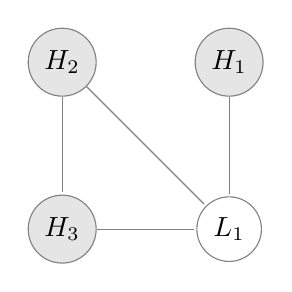
\begin{tikzpicture}[shorten >=1pt,draw=black!50]
	\node (H1) at ( 1.06,  1.06)	[circle, draw, fill = gray!20]	{$H_{1}$};
	\node (H2) at (-1.06,  1.06)	[circle, draw, fill = gray!20]	{$H_{2}$};
	\node (H3) at (-1.06, -1.06)	[circle, draw, fill = gray!20]	{$H_{3}$};
	\node (L1) at ( 1.06, -1.06)	[circle, draw, fill = white]	{$L_{1}$};
	\draw (H1) -- (L1);
	\draw (H2) -- (H3);
	\draw (H2) -- (L1);
	\draw (H3) -- (L1);
\end{tikzpicture}
\end{center}
\columnbreak

\scaleeq{
Equations: \begin{cases}
	e^{H}_{1} \left(\frac{25 \phi}{3} - 3\right) = \alpha - 3 e^{H}_{2} - 3 e^{H}_{3} + e^{L}_{1} \theta - \gamma\\
	e^{H}_{2} \left(\frac{25 \phi}{2} - 2\right) = \alpha - 2 e^{H}_{1} + 2 e^{H}_{3} + e^{L}_{1} \theta - \gamma\\
	e^{H}_{3} \left(\frac{25 \phi}{2} - 2\right) = \alpha - 2 e^{H}_{1} + 2 e^{H}_{2} + e^{L}_{1} \theta - \gamma\\
	e^{L}_{1} \left(\frac{25 \phi}{\theta} - \theta\right) = \alpha + 3 e^{H}_{1} + 2 e^{H}_{2} + 2 e^{H}_{3} - \gamma
\end{cases}
}\end{multicols}


Optimal efforts:

\scaleeq{
\begin{cases}
	e^{H}_{1} &= \frac{15 \phi \left(\alpha - \gamma\right) \left(5 \phi - 4\right)}{625 \phi^{3} - 25 \phi^{2} \theta^{2} - 425 \phi^{2} + 12 \theta^{2}}\\
	e^{H}_{2} &= \frac{10 \phi \left(\alpha - \gamma\right) \left(5 \phi - 3\right)}{625 \phi^{3} - 25 \phi^{2} \theta^{2} - 425 \phi^{2} + 12 \theta^{2}}\\
	e^{H}_{3} &= \frac{10 \phi \left(\alpha - \gamma\right) \left(5 \phi - 3\right)}{625 \phi^{3} - 25 \phi^{2} \theta^{2} - 425 \phi^{2} + 12 \theta^{2}}\\
	e^{L}_{1} &= \frac{\theta \left(\alpha - \gamma\right) \left(25 \phi^{2} - 12\right)}{625 \phi^{3} - 25 \phi^{2} \theta^{2} - 425 \phi^{2} + 12 \theta^{2}}
\end{cases}
}

Production Costs:

\scaleeq{
\begin{cases}
	c^{H}_{1} &= - \frac{25 \alpha \phi^{2} \theta^{2} + 75 \alpha \phi^{2} - 60 \alpha \phi - 12 \alpha \theta^{2} - 625 \gamma \phi^{3} + 350 \gamma \phi^{2} + 60 \gamma \phi}{625 \phi^{3} - 25 \phi^{2} \theta^{2} - 425 \phi^{2} + 12 \theta^{2}}\\
	c^{H}_{2} &= - \frac{25 \alpha \phi^{2} \theta^{2} + 100 \alpha \phi^{2} - 60 \alpha \phi - 12 \alpha \theta^{2} - 625 \gamma \phi^{3} + 325 \gamma \phi^{2} + 60 \gamma \phi}{625 \phi^{3} - 25 \phi^{2} \theta^{2} - 425 \phi^{2} + 12 \theta^{2}}\\
	c^{H}_{3} &= - \frac{25 \alpha \phi^{2} \theta^{2} + 100 \alpha \phi^{2} - 60 \alpha \phi - 12 \alpha \theta^{2} - 625 \gamma \phi^{3} + 325 \gamma \phi^{2} + 60 \gamma \phi}{625 \phi^{3} - 25 \phi^{2} \theta^{2} - 425 \phi^{2} + 12 \theta^{2}}\\
	c^{L}_{1} &= - \frac{25 \alpha \phi^{2} \theta^{2} + 175 \alpha \phi^{2} - 120 \alpha \phi - 12 \alpha \theta^{2} - 625 \gamma \phi^{3} + 250 \gamma \phi^{2} + 120 \gamma \phi}{625 \phi^{3} - 25 \phi^{2} \theta^{2} - 425 \phi^{2} + 12 \theta^{2}}
\end{cases}
}

Production Quantities:

\scaleeq{
\begin{cases}
	q^{H}_{1} &= \frac{25 \phi^{2} \left(\alpha - \gamma\right) \left(5 \phi - 4\right)}{625 \phi^{3} - 25 \phi^{2} \theta^{2} - 425 \phi^{2} + 12 \theta^{2}}\\
	q^{H}_{2} &= \frac{25 \phi^{2} \left(\alpha - \gamma\right) \left(5 \phi - 3\right)}{625 \phi^{3} - 25 \phi^{2} \theta^{2} - 425 \phi^{2} + 12 \theta^{2}}\\
	q^{H}_{3} &= \frac{25 \phi^{2} \left(\alpha - \gamma\right) \left(5 \phi - 3\right)}{625 \phi^{3} - 25 \phi^{2} \theta^{2} - 425 \phi^{2} + 12 \theta^{2}}\\
	q^{L}_{1} &= \frac{5 \phi \left(\alpha - \gamma\right) \left(25 \phi^{2} - 12\right)}{625 \phi^{3} - 25 \phi^{2} \theta^{2} - 425 \phi^{2} + 12 \theta^{2}}
\end{cases}
}

Profits:

\begin{equation}
\label{eq:E4D:3H1L_profit}
\scaledequation{\begin{cases}
	\pi^{H}_{1} &= \frac{25 \phi^{3} \left(\alpha - \gamma\right)^{2} \left(5 \phi - 4\right)^{2} \left(25 \phi - 9\right)}{\left(625 \phi^{3} - 25 \phi^{2} \theta^{2} - 425 \phi^{2} + 12 \theta^{2}\right)^{2}}\\
	\pi^{H}_{2} &= \frac{25 \phi^{3} \left(\alpha - \gamma\right)^{2} \left(5 \phi - 3\right)^{2} \left(25 \phi - 4\right)}{\left(625 \phi^{3} - 25 \phi^{2} \theta^{2} - 425 \phi^{2} + 12 \theta^{2}\right)^{2}}\\
	\pi^{H}_{3} &= \frac{25 \phi^{3} \left(\alpha - \gamma\right)^{2} \left(5 \phi - 3\right)^{2} \left(25 \phi - 4\right)}{\left(625 \phi^{3} - 25 \phi^{2} \theta^{2} - 425 \phi^{2} + 12 \theta^{2}\right)^{2}}\\
	\pi^{L}_{1} &= \frac{\phi \left(\alpha - \gamma\right)^{2} \left(25 \phi - \theta^{2}\right) \left(25 \phi^{2} - 12\right)^{2}}{\left(625 \phi^{3} - 25 \phi^{2} \theta^{2} - 425 \phi^{2} + 12 \theta^{2}\right)^{2}}
\end{cases}
}
\end{equation}

Total Production:

\scaleeq{
\frac{10 \phi \left(\alpha - \gamma\right) \left(50 \phi^{2} - 25 \phi - 6\right)}{625 \phi^{3} - 25 \phi^{2} \theta^{2} - 425 \phi^{2} + 12 \theta^{2}}
}

Price:

\scaleeq{
\frac{125 \alpha \phi^{3} - 25 \alpha \phi^{2} \theta^{2} - 175 \alpha \phi^{2} + 60 \alpha \phi + 12 \alpha \theta^{2} + 500 \gamma \phi^{3} - 250 \gamma \phi^{2} - 60 \gamma \phi}{625 \phi^{3} - 25 \phi^{2} \theta^{2} - 425 \phi^{2} + 12 \theta^{2}}
}

Firm Surplus:

\scaleeq{
\frac{\phi \left(\alpha - \gamma\right)^{2} \left(62500 \phi^{5} - 625 \phi^{4} \theta^{2} - 73125 \phi^{4} + 21250 \phi^{3} + 600 \phi^{2} \theta^{2} - 5400 \phi^{2} + 3600 \phi - 144 \theta^{2}\right)}{\left(625 \phi^{3} - 25 \phi^{2} \theta^{2} - 425 \phi^{2} + 12 \theta^{2}\right)^{2}}
}

Consumer Surplus:

\scaleeq{
\frac{50 \phi^{2} \left(\alpha - \gamma\right)^{2} \left(50 \phi^{2} - 25 \phi - 6\right)^{2}}{\left(625 \phi^{3} - 25 \phi^{2} \theta^{2} - 425 \phi^{2} + 12 \theta^{2}\right)^{2}}
}

Social Welfare:

\scaleeq{
\frac{\phi \left(\alpha - \gamma\right)^{2} \left(187500 \phi^{5} - 625 \phi^{4} \theta^{2} - 198125 \phi^{4} + 22500 \phi^{3} + 600 \phi^{2} \theta^{2} + 9600 \phi^{2} + 5400 \phi - 144 \theta^{2}\right)}{\left(625 \phi^{3} - 25 \phi^{2} \theta^{2} - 425 \phi^{2} + 12 \theta^{2}\right)^{2}}
}

%======================================================================

\subsubsection{E5A [3H1L]}
\label{apx:E5A:3H1L}

\begin{multicols}{2}
\begin{center}
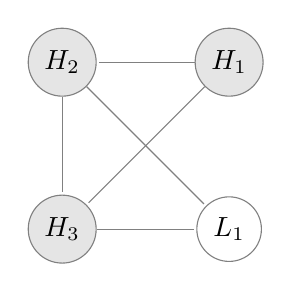
\begin{tikzpicture}[shorten >=1pt,draw=black!50]
	\node (H1) at ( 1.06,  1.06)	[circle, draw, fill = gray!20]	{$H_{1}$};
	\node (H2) at (-1.06,  1.06)	[circle, draw, fill = gray!20]	{$H_{2}$};
	\node (H3) at (-1.06, -1.06)	[circle, draw, fill = gray!20]	{$H_{3}$};
	\node (L1) at ( 1.06, -1.06)	[circle, draw, fill = white]	{$L_{1}$};
	\draw (H1) -- (H2);
	\draw (H1) -- (H3);
	\draw (H2) -- (H3);
	\draw (H2) -- (L1);
	\draw (H3) -- (L1);
\end{tikzpicture}
\end{center}
\columnbreak

\scaleeq{
Equations: \begin{cases}
	e^{H}_{1} \left(\frac{25 \phi}{2} - 2\right) = \alpha + e^{H}_{2} + e^{H}_{3} - 3 e^{L}_{1} \theta - \gamma\\
	e^{H}_{2} \left(25 \phi - 1\right) = \alpha + 2 e^{H}_{1} + e^{H}_{3} + 2 e^{L}_{1} \theta - \gamma\\
	e^{H}_{3} \left(25 \phi - 1\right) = \alpha + 2 e^{H}_{1} + e^{H}_{2} + 2 e^{L}_{1} \theta - \gamma\\
	e^{L}_{1} \left(\frac{25 \phi}{2 \theta} - 2 \theta\right) = \alpha - 3 e^{H}_{1} + e^{H}_{2} + e^{H}_{3} - \gamma
\end{cases}
}\end{multicols}


Optimal efforts:

\scaleeq{
\begin{cases}
	e^{H}_{1} &= \frac{10 \phi \left(\alpha - \gamma\right) \left(5 \phi - 2 \theta^{2}\right)}{625 \phi^{3} - 100 \phi^{2} \theta^{2} - 150 \phi^{2} - 20 \phi \theta^{2} + 8 \theta^{2}}\\
	e^{H}_{2} &= \frac{\left(\alpha - \gamma\right) \left(5 \phi - 2 \theta\right) \left(5 \phi + 2 \theta\right)}{625 \phi^{3} - 100 \phi^{2} \theta^{2} - 150 \phi^{2} - 20 \phi \theta^{2} + 8 \theta^{2}}\\
	e^{H}_{3} &= \frac{\left(\alpha - \gamma\right) \left(5 \phi - 2 \theta\right) \left(5 \phi + 2 \theta\right)}{625 \phi^{3} - 100 \phi^{2} \theta^{2} - 150 \phi^{2} - 20 \phi \theta^{2} + 8 \theta^{2}}\\
	e^{L}_{1} &= \frac{10 \phi \theta \left(\alpha - \gamma\right) \left(5 \phi - 2\right)}{625 \phi^{3} - 100 \phi^{2} \theta^{2} - 150 \phi^{2} - 20 \phi \theta^{2} + 8 \theta^{2}}
\end{cases}
}

Production Costs:

\scaleeq{
\begin{cases}
	c^{H}_{1} &= - \frac{100 \alpha \phi^{2} - 20 \alpha \phi \theta^{2} - 8 \alpha \theta^{2} - 625 \gamma \phi^{3} + 100 \gamma \phi^{2} \theta^{2} + 50 \gamma \phi^{2} + 40 \gamma \phi \theta^{2}}{625 \phi^{3} - 100 \phi^{2} \theta^{2} - 150 \phi^{2} - 20 \phi \theta^{2} + 8 \theta^{2}}\\
	c^{H}_{2} &= - \frac{50 \alpha \phi^{2} \theta^{2} + 100 \alpha \phi^{2} - 40 \alpha \phi \theta^{2} - 8 \alpha \theta^{2} - 625 \gamma \phi^{3} + 50 \gamma \phi^{2} \theta^{2} + 50 \gamma \phi^{2} + 60 \gamma \phi \theta^{2}}{625 \phi^{3} - 100 \phi^{2} \theta^{2} - 150 \phi^{2} - 20 \phi \theta^{2} + 8 \theta^{2}}\\
	c^{H}_{3} &= - \frac{50 \alpha \phi^{2} \theta^{2} + 100 \alpha \phi^{2} - 40 \alpha \phi \theta^{2} - 8 \alpha \theta^{2} - 625 \gamma \phi^{3} + 50 \gamma \phi^{2} \theta^{2} + 50 \gamma \phi^{2} + 60 \gamma \phi \theta^{2}}{625 \phi^{3} - 100 \phi^{2} \theta^{2} - 150 \phi^{2} - 20 \phi \theta^{2} + 8 \theta^{2}}\\
	c^{L}_{1} &= - \frac{50 \alpha \phi^{2} \theta^{2} + 50 \alpha \phi^{2} - 20 \alpha \phi \theta^{2} - 8 \alpha \theta^{2} - 625 \gamma \phi^{3} + 50 \gamma \phi^{2} \theta^{2} + 100 \gamma \phi^{2} + 40 \gamma \phi \theta^{2}}{625 \phi^{3} - 100 \phi^{2} \theta^{2} - 150 \phi^{2} - 20 \phi \theta^{2} + 8 \theta^{2}}
\end{cases}
}

Production Quantities:

\scaleeq{
\begin{cases}
	q^{H}_{1} &= \frac{25 \phi^{2} \left(\alpha - \gamma\right) \left(5 \phi - 2 \theta^{2}\right)}{625 \phi^{3} - 100 \phi^{2} \theta^{2} - 150 \phi^{2} - 20 \phi \theta^{2} + 8 \theta^{2}}\\
	q^{H}_{2} &= \frac{5 \phi \left(\alpha - \gamma\right) \left(5 \phi - 2 \theta\right) \left(5 \phi + 2 \theta\right)}{625 \phi^{3} - 100 \phi^{2} \theta^{2} - 150 \phi^{2} - 20 \phi \theta^{2} + 8 \theta^{2}}\\
	q^{H}_{3} &= \frac{5 \phi \left(\alpha - \gamma\right) \left(5 \phi - 2 \theta\right) \left(5 \phi + 2 \theta\right)}{625 \phi^{3} - 100 \phi^{2} \theta^{2} - 150 \phi^{2} - 20 \phi \theta^{2} + 8 \theta^{2}}\\
	q^{L}_{1} &= \frac{25 \phi^{2} \left(\alpha - \gamma\right) \left(5 \phi - 2\right)}{625 \phi^{3} - 100 \phi^{2} \theta^{2} - 150 \phi^{2} - 20 \phi \theta^{2} + 8 \theta^{2}}
\end{cases}
}

Profits:

\begin{equation}
\label{eq:E5A:3H1L_profit}
\scaledequation{\begin{cases}
	\pi^{H}_{1} &= \frac{25 \phi^{3} \left(\alpha - \gamma\right)^{2} \left(5 \phi - 2 \theta^{2}\right)^{2} \left(25 \phi - 4\right)}{\left(625 \phi^{3} - 100 \phi^{2} \theta^{2} - 150 \phi^{2} - 20 \phi \theta^{2} + 8 \theta^{2}\right)^{2}}\\
	\pi^{H}_{2} &= \frac{\phi \left(\alpha - \gamma\right)^{2} \left(5 \phi - 2 \theta\right)^{2} \left(5 \phi + 2 \theta\right)^{2} \left(25 \phi - 1\right)}{\left(625 \phi^{3} - 100 \phi^{2} \theta^{2} - 150 \phi^{2} - 20 \phi \theta^{2} + 8 \theta^{2}\right)^{2}}\\
	\pi^{H}_{3} &= \frac{\phi \left(\alpha - \gamma\right)^{2} \left(5 \phi - 2 \theta\right)^{2} \left(5 \phi + 2 \theta\right)^{2} \left(25 \phi - 1\right)}{\left(625 \phi^{3} - 100 \phi^{2} \theta^{2} - 150 \phi^{2} - 20 \phi \theta^{2} + 8 \theta^{2}\right)^{2}}\\
	\pi^{L}_{1} &= \frac{25 \phi^{3} \left(\alpha - \gamma\right)^{2} \left(5 \phi - 2\right)^{2} \left(25 \phi - 4 \theta^{2}\right)}{\left(625 \phi^{3} - 100 \phi^{2} \theta^{2} - 150 \phi^{2} - 20 \phi \theta^{2} + 8 \theta^{2}\right)^{2}}
\end{cases}
}
\end{equation}

Total Production:

\scaleeq{
\frac{10 \phi \left(\alpha - \gamma\right) \left(50 \phi^{2} - 5 \phi \theta^{2} - 5 \phi - 4 \theta^{2}\right)}{625 \phi^{3} - 100 \phi^{2} \theta^{2} - 150 \phi^{2} - 20 \phi \theta^{2} + 8 \theta^{2}}
}

Price:

\scaleeq{
\frac{125 \alpha \phi^{3} - 50 \alpha \phi^{2} \theta^{2} - 100 \alpha \phi^{2} + 20 \alpha \phi \theta^{2} + 8 \alpha \theta^{2} + 500 \gamma \phi^{3} - 50 \gamma \phi^{2} \theta^{2} - 50 \gamma \phi^{2} - 40 \gamma \phi \theta^{2}}{625 \phi^{3} - 100 \phi^{2} \theta^{2} - 150 \phi^{2} - 20 \phi \theta^{2} + 8 \theta^{2}}
}

Firm Surplus:

\scaleeq{
\frac{2 \phi \left(\alpha - \gamma\right)^{2} \left(31250 \phi^{5} - 7500 \phi^{4} \theta^{2} - 8125 \phi^{4} + 1250 \phi^{3} \theta^{4} - 3000 \phi^{3} \theta^{2} + 1250 \phi^{3} - 200 \phi^{2} \theta^{4} + 400 \phi \theta^{4} - 16 \theta^{4}\right)}{\left(625 \phi^{3} - 100 \phi^{2} \theta^{2} - 150 \phi^{2} - 20 \phi \theta^{2} + 8 \theta^{2}\right)^{2}}
}

Consumer Surplus:

\scaleeq{
\frac{50 \phi^{2} \left(\alpha - \gamma\right)^{2} \left(50 \phi^{2} - 5 \phi \theta^{2} - 5 \phi - 4 \theta^{2}\right)^{2}}{\left(625 \phi^{3} - 100 \phi^{2} \theta^{2} - 150 \phi^{2} - 20 \phi \theta^{2} + 8 \theta^{2}\right)^{2}}
}

Social Welfare:

\scaleeq{
\frac{2 \phi \left(\alpha - \gamma\right)^{2} \left(93750 \phi^{5} - 20000 \phi^{4} \theta^{2} - 20625 \phi^{4} + 1875 \phi^{3} \theta^{4} - 11750 \phi^{3} \theta^{2} + 1875 \phi^{3} + 800 \phi^{2} \theta^{4} + 1000 \phi^{2} \theta^{2} + 800 \phi \theta^{4} - 16 \theta^{4}\right)}{\left(625 \phi^{3} - 100 \phi^{2} \theta^{2} - 150 \phi^{2} - 20 \phi \theta^{2} + 8 \theta^{2}\right)^{2}}
}

%======================================================================

\subsubsection{E5B [3H1L]}
\label{apx:E5B:3H1L}

\begin{multicols}{2}
\begin{center}
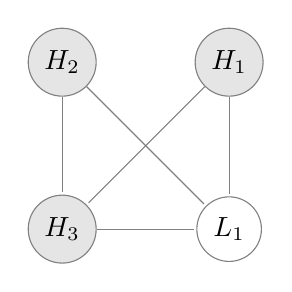
\begin{tikzpicture}[shorten >=1pt,draw=black!50]
	\node (H1) at ( 1.06,  1.06)	[circle, draw, fill = gray!20]	{$H_{1}$};
	\node (H2) at (-1.06,  1.06)	[circle, draw, fill = gray!20]	{$H_{2}$};
	\node (H3) at (-1.06, -1.06)	[circle, draw, fill = gray!20]	{$H_{3}$};
	\node (L1) at ( 1.06, -1.06)	[circle, draw, fill = white]	{$L_{1}$};
	\draw (H1) -- (H3);
	\draw (H1) -- (L1);
	\draw (H2) -- (H3);
	\draw (H2) -- (L1);
	\draw (H3) -- (L1);
\end{tikzpicture}
\end{center}
\columnbreak

\scaleeq{
Equations: \begin{cases}
	e^{H}_{1} \left(\frac{25 \phi}{2} - 2\right) = \alpha - 3 e^{H}_{2} + e^{H}_{3} + e^{L}_{1} \theta - \gamma\\
	e^{H}_{2} \left(\frac{25 \phi}{2} - 2\right) = \alpha - 3 e^{H}_{1} + e^{H}_{3} + e^{L}_{1} \theta - \gamma\\
	e^{H}_{3} \left(25 \phi - 1\right) = \alpha + 2 e^{H}_{1} + 2 e^{H}_{2} + e^{L}_{1} \theta - \gamma\\
	e^{L}_{1} \left(\frac{25 \phi}{\theta} - \theta\right) = \alpha + 2 e^{H}_{1} + 2 e^{H}_{2} + e^{H}_{3} - \gamma
\end{cases}
}\end{multicols}


Optimal efforts:

\scaleeq{
\begin{cases}
	e^{H}_{1} &= \frac{10 \phi \left(\alpha - \gamma\right)}{125 \phi^{2} - 5 \phi \theta^{2} + 5 \phi - 2 \theta^{2} - 2}\\
	e^{H}_{2} &= \frac{10 \phi \left(\alpha - \gamma\right)}{125 \phi^{2} - 5 \phi \theta^{2} + 5 \phi - 2 \theta^{2} - 2}\\
	e^{H}_{3} &= \frac{\left(\alpha - \gamma\right) \left(5 \phi + 2\right)}{125 \phi^{2} - 5 \phi \theta^{2} + 5 \phi - 2 \theta^{2} - 2}\\
	e^{L}_{1} &= \frac{\theta \left(\alpha - \gamma\right) \left(5 \phi + 2\right)}{125 \phi^{2} - 5 \phi \theta^{2} + 5 \phi - 2 \theta^{2} - 2}
\end{cases}
}

Production Costs:

\scaleeq{
\begin{cases}
	c^{H}_{1} &= - \frac{5 \alpha \phi \theta^{2} + 15 \alpha \phi + 2 \alpha \theta^{2} + 2 \alpha - 125 \gamma \phi^{2} - 20 \gamma \phi}{125 \phi^{2} - 5 \phi \theta^{2} + 5 \phi - 2 \theta^{2} - 2}\\
	c^{H}_{2} &= - \frac{5 \alpha \phi \theta^{2} + 15 \alpha \phi + 2 \alpha \theta^{2} + 2 \alpha - 125 \gamma \phi^{2} - 20 \gamma \phi}{125 \phi^{2} - 5 \phi \theta^{2} + 5 \phi - 2 \theta^{2} - 2}\\
	c^{H}_{3} &= - \frac{5 \alpha \phi \theta^{2} + 25 \alpha \phi + 2 \alpha \theta^{2} + 2 \alpha - 125 \gamma \phi^{2} - 30 \gamma \phi}{125 \phi^{2} - 5 \phi \theta^{2} + 5 \phi - 2 \theta^{2} - 2}\\
	c^{L}_{1} &= - \frac{5 \alpha \phi \theta^{2} + 25 \alpha \phi + 2 \alpha \theta^{2} + 2 \alpha - 125 \gamma \phi^{2} - 30 \gamma \phi}{125 \phi^{2} - 5 \phi \theta^{2} + 5 \phi - 2 \theta^{2} - 2}
\end{cases}
}

Production Quantities:

\scaleeq{
\begin{cases}
	q^{H}_{1} &= \frac{25 \phi^{2} \left(\alpha - \gamma\right)}{125 \phi^{2} - 5 \phi \theta^{2} + 5 \phi - 2 \theta^{2} - 2}\\
	q^{H}_{2} &= \frac{25 \phi^{2} \left(\alpha - \gamma\right)}{125 \phi^{2} - 5 \phi \theta^{2} + 5 \phi - 2 \theta^{2} - 2}\\
	q^{H}_{3} &= \frac{5 \phi \left(\alpha - \gamma\right) \left(5 \phi + 2\right)}{125 \phi^{2} - 5 \phi \theta^{2} + 5 \phi - 2 \theta^{2} - 2}\\
	q^{L}_{1} &= \frac{5 \phi \left(\alpha - \gamma\right) \left(5 \phi + 2\right)}{125 \phi^{2} - 5 \phi \theta^{2} + 5 \phi - 2 \theta^{2} - 2}
\end{cases}
}

Profits:

\begin{equation}
\label{eq:E5B:3H1L_profit}
\scaledequation{\begin{cases}
	\pi^{H}_{1} &= \frac{25 \phi^{3} \left(\alpha - \gamma\right)^{2} \left(25 \phi - 4\right)}{\left(125 \phi^{2} - 5 \phi \theta^{2} + 5 \phi - 2 \theta^{2} - 2\right)^{2}}\\
	\pi^{H}_{2} &= \frac{25 \phi^{3} \left(\alpha - \gamma\right)^{2} \left(25 \phi - 4\right)}{\left(125 \phi^{2} - 5 \phi \theta^{2} + 5 \phi - 2 \theta^{2} - 2\right)^{2}}\\
	\pi^{H}_{3} &= \frac{\phi \left(\alpha - \gamma\right)^{2} \left(5 \phi + 2\right)^{2} \left(25 \phi - 1\right)}{\left(125 \phi^{2} - 5 \phi \theta^{2} + 5 \phi - 2 \theta^{2} - 2\right)^{2}}\\
	\pi^{L}_{1} &= \frac{\phi \left(\alpha - \gamma\right)^{2} \left(5 \phi + 2\right)^{2} \left(25 \phi - \theta^{2}\right)}{\left(125 \phi^{2} - 5 \phi \theta^{2} + 5 \phi - 2 \theta^{2} - 2\right)^{2}}
\end{cases}
}
\end{equation}

Total Production:

\scaleeq{
\frac{20 \phi \left(\alpha - \gamma\right) \left(5 \phi + 1\right)}{125 \phi^{2} - 5 \phi \theta^{2} + 5 \phi - 2 \theta^{2} - 2}
}

Price:

\scaleeq{
\frac{25 \alpha \phi^{2} - 5 \alpha \phi \theta^{2} - 15 \alpha \phi - 2 \alpha \theta^{2} - 2 \alpha + 100 \gamma \phi^{2} + 20 \gamma \phi}{125 \phi^{2} - 5 \phi \theta^{2} + 5 \phi - 2 \theta^{2} - 2}
}

Firm Surplus:

\scaleeq{
\frac{\phi \left(\alpha - \gamma\right)^{2} \left(2500 \phi^{3} - 25 \phi^{2} \theta^{2} + 775 \phi^{2} - 20 \phi \theta^{2} + 180 \phi - 4 \theta^{2} - 4\right)}{\left(125 \phi^{2} - 5 \phi \theta^{2} + 5 \phi - 2 \theta^{2} - 2\right)^{2}}
}

Consumer Surplus:

\scaleeq{
\frac{200 \phi^{2} \left(\alpha - \gamma\right)^{2} \left(5 \phi + 1\right)^{2}}{\left(125 \phi^{2} - 5 \phi \theta^{2} + 5 \phi - 2 \theta^{2} - 2\right)^{2}}
}

Social Welfare:

\scaleeq{
\frac{\phi \left(\alpha - \gamma\right)^{2} \left(7500 \phi^{3} - 25 \phi^{2} \theta^{2} + 2775 \phi^{2} - 20 \phi \theta^{2} + 380 \phi - 4 \theta^{2} - 4\right)}{\left(125 \phi^{2} - 5 \phi \theta^{2} + 5 \phi - 2 \theta^{2} - 2\right)^{2}}
}

%======================================================================

\subsubsection{E6A [3H1L]}
\label{apx:E6A:3H1L}

\begin{multicols}{2}
\begin{center}
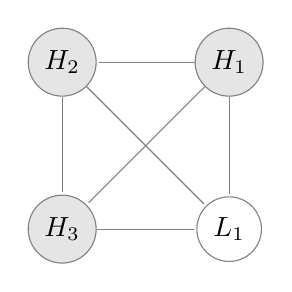
\begin{tikzpicture}[shorten >=1pt,draw=black!50]
	\node (H1) at ( 1.06,  1.06)	[circle, draw, fill = gray!20]	{$H_{1}$};
	\node (H2) at (-1.06,  1.06)	[circle, draw, fill = gray!20]	{$H_{2}$};
	\node (H3) at (-1.06, -1.06)	[circle, draw, fill = gray!20]	{$H_{3}$};
	\node (L1) at ( 1.06, -1.06)	[circle, draw, fill = white]	{$L_{1}$};
	\draw (H1) -- (H2);
	\draw (H1) -- (H3);
	\draw (H1) -- (L1);
	\draw (H2) -- (H3);
	\draw (H2) -- (L1);
	\draw (H3) -- (L1);
\end{tikzpicture}
\end{center}
\columnbreak

\scaleeq{
Equations: \begin{cases}
	e^{H}_{1} \left(25 \phi - 1\right) = \alpha + e^{H}_{2} + e^{H}_{3} + e^{L}_{1} \theta - \gamma\\
	e^{H}_{2} \left(25 \phi - 1\right) = \alpha + e^{H}_{1} + e^{H}_{3} + e^{L}_{1} \theta - \gamma\\
	e^{H}_{3} \left(25 \phi - 1\right) = \alpha + e^{H}_{1} + e^{H}_{2} + e^{L}_{1} \theta - \gamma\\
	e^{L}_{1} \left(\frac{25 \phi}{\theta} - \theta\right) = \alpha + e^{H}_{1} + e^{H}_{2} + e^{H}_{3} - \gamma
\end{cases}
}\end{multicols}


Optimal efforts:

\scaleeq{
\begin{cases}
	e^{H}_{1} &= \frac{\alpha - \gamma}{25 \phi - \theta^{2} - 3}\\
	e^{H}_{2} &= \frac{\alpha - \gamma}{25 \phi - \theta^{2} - 3}\\
	e^{H}_{3} &= \frac{\alpha - \gamma}{25 \phi - \theta^{2} - 3}\\
	e^{L}_{1} &= \frac{\theta \left(\alpha - \gamma\right)}{25 \phi - \theta^{2} - 3}
\end{cases}
}

Production Costs:

\scaleeq{
\begin{cases}
	c^{H}_{1} &= - \frac{\alpha \theta^{2} + 3 \alpha - 25 \gamma \phi}{25 \phi - \theta^{2} - 3}\\
	c^{H}_{2} &= - \frac{\alpha \theta^{2} + 3 \alpha - 25 \gamma \phi}{25 \phi - \theta^{2} - 3}\\
	c^{H}_{3} &= - \frac{\alpha \theta^{2} + 3 \alpha - 25 \gamma \phi}{25 \phi - \theta^{2} - 3}\\
	c^{L}_{1} &= - \frac{\alpha \theta^{2} + 3 \alpha - 25 \gamma \phi}{25 \phi - \theta^{2} - 3}
\end{cases}
}

Production Quantities:

\scaleeq{
\begin{cases}
	q^{H}_{1} &= \frac{5 \phi \left(\alpha - \gamma\right)}{25 \phi - \theta^{2} - 3}\\
	q^{H}_{2} &= \frac{5 \phi \left(\alpha - \gamma\right)}{25 \phi - \theta^{2} - 3}\\
	q^{H}_{3} &= \frac{5 \phi \left(\alpha - \gamma\right)}{25 \phi - \theta^{2} - 3}\\
	q^{L}_{1} &= \frac{5 \phi \left(\alpha - \gamma\right)}{25 \phi - \theta^{2} - 3}
\end{cases}
}

Profits:

\begin{equation}
\label{eq:E6A:3H1L_profit}
\scaledequation{\begin{cases}
	\pi^{H}_{1} &= \frac{\phi \left(\alpha - \gamma\right)^{2} \left(25 \phi - 1\right)}{\left(25 \phi - \theta^{2} - 3\right)^{2}}\\
	\pi^{H}_{2} &= \frac{\phi \left(\alpha - \gamma\right)^{2} \left(25 \phi - 1\right)}{\left(25 \phi - \theta^{2} - 3\right)^{2}}\\
	\pi^{H}_{3} &= \frac{\phi \left(\alpha - \gamma\right)^{2} \left(25 \phi - 1\right)}{\left(25 \phi - \theta^{2} - 3\right)^{2}}\\
	\pi^{L}_{1} &= \frac{\phi \left(\alpha - \gamma\right)^{2} \left(25 \phi - \theta^{2}\right)}{\left(25 \phi - \theta^{2} - 3\right)^{2}}
\end{cases}
}
\end{equation}

Total Production:

\scaleeq{
\frac{20 \phi \left(\alpha - \gamma\right)}{25 \phi - \theta^{2} - 3}
}

Price:

\scaleeq{
\frac{5 \alpha \phi - \alpha \theta^{2} - 3 \alpha + 20 \gamma \phi}{25 \phi - \theta^{2} - 3}
}

Firm Surplus:

\scaleeq{
\frac{\phi \left(\alpha - \gamma\right)^{2} \left(100 \phi - \theta^{2} - 3\right)}{\left(25 \phi - \theta^{2} - 3\right)^{2}}
}

Consumer Surplus:

\scaleeq{
\frac{200 \phi^{2} \left(\alpha - \gamma\right)^{2}}{\left(25 \phi - \theta^{2} - 3\right)^{2}}
}

Social Welfare:

\scaleeq{
\frac{\phi \left(\alpha - \gamma\right)^{2} \left(300 \phi - \theta^{2} - 3\right)}{\left(25 \phi - \theta^{2} - 3\right)^{2}}
}

%======================================================================

